% Options for packages loaded elsewhere
% Options for packages loaded elsewhere
\PassOptionsToPackage{unicode}{hyperref}
\PassOptionsToPackage{hyphens}{url}
\PassOptionsToPackage{dvipsnames,svgnames,x11names}{xcolor}
%
\documentclass[
  letterpaper,
  DIV=11,
  numbers=noendperiod]{scrreprt}
\usepackage{xcolor}
\usepackage{amsmath,amssymb}
\setcounter{secnumdepth}{5}
\usepackage{iftex}
\ifPDFTeX
  \usepackage[T1]{fontenc}
  \usepackage[utf8]{inputenc}
  \usepackage{textcomp} % provide euro and other symbols
\else % if luatex or xetex
  \usepackage{unicode-math} % this also loads fontspec
  \defaultfontfeatures{Scale=MatchLowercase}
  \defaultfontfeatures[\rmfamily]{Ligatures=TeX,Scale=1}
\fi
\usepackage{lmodern}
\ifPDFTeX\else
  % xetex/luatex font selection
\fi
% Use upquote if available, for straight quotes in verbatim environments
\IfFileExists{upquote.sty}{\usepackage{upquote}}{}
\IfFileExists{microtype.sty}{% use microtype if available
  \usepackage[]{microtype}
  \UseMicrotypeSet[protrusion]{basicmath} % disable protrusion for tt fonts
}{}
\makeatletter
\@ifundefined{KOMAClassName}{% if non-KOMA class
  \IfFileExists{parskip.sty}{%
    \usepackage{parskip}
  }{% else
    \setlength{\parindent}{0pt}
    \setlength{\parskip}{6pt plus 2pt minus 1pt}}
}{% if KOMA class
  \KOMAoptions{parskip=half}}
\makeatother
% Make \paragraph and \subparagraph free-standing
\makeatletter
\ifx\paragraph\undefined\else
  \let\oldparagraph\paragraph
  \renewcommand{\paragraph}{
    \@ifstar
      \xxxParagraphStar
      \xxxParagraphNoStar
  }
  \newcommand{\xxxParagraphStar}[1]{\oldparagraph*{#1}\mbox{}}
  \newcommand{\xxxParagraphNoStar}[1]{\oldparagraph{#1}\mbox{}}
\fi
\ifx\subparagraph\undefined\else
  \let\oldsubparagraph\subparagraph
  \renewcommand{\subparagraph}{
    \@ifstar
      \xxxSubParagraphStar
      \xxxSubParagraphNoStar
  }
  \newcommand{\xxxSubParagraphStar}[1]{\oldsubparagraph*{#1}\mbox{}}
  \newcommand{\xxxSubParagraphNoStar}[1]{\oldsubparagraph{#1}\mbox{}}
\fi
\makeatother

\usepackage{color}
\usepackage{fancyvrb}
\newcommand{\VerbBar}{|}
\newcommand{\VERB}{\Verb[commandchars=\\\{\}]}
\DefineVerbatimEnvironment{Highlighting}{Verbatim}{commandchars=\\\{\}}
% Add ',fontsize=\small' for more characters per line
\usepackage{framed}
\definecolor{shadecolor}{RGB}{241,243,245}
\newenvironment{Shaded}{\begin{snugshade}}{\end{snugshade}}
\newcommand{\AlertTok}[1]{\textcolor[rgb]{0.68,0.00,0.00}{#1}}
\newcommand{\AnnotationTok}[1]{\textcolor[rgb]{0.37,0.37,0.37}{#1}}
\newcommand{\AttributeTok}[1]{\textcolor[rgb]{0.40,0.45,0.13}{#1}}
\newcommand{\BaseNTok}[1]{\textcolor[rgb]{0.68,0.00,0.00}{#1}}
\newcommand{\BuiltInTok}[1]{\textcolor[rgb]{0.00,0.23,0.31}{#1}}
\newcommand{\CharTok}[1]{\textcolor[rgb]{0.13,0.47,0.30}{#1}}
\newcommand{\CommentTok}[1]{\textcolor[rgb]{0.37,0.37,0.37}{#1}}
\newcommand{\CommentVarTok}[1]{\textcolor[rgb]{0.37,0.37,0.37}{\textit{#1}}}
\newcommand{\ConstantTok}[1]{\textcolor[rgb]{0.56,0.35,0.01}{#1}}
\newcommand{\ControlFlowTok}[1]{\textcolor[rgb]{0.00,0.23,0.31}{\textbf{#1}}}
\newcommand{\DataTypeTok}[1]{\textcolor[rgb]{0.68,0.00,0.00}{#1}}
\newcommand{\DecValTok}[1]{\textcolor[rgb]{0.68,0.00,0.00}{#1}}
\newcommand{\DocumentationTok}[1]{\textcolor[rgb]{0.37,0.37,0.37}{\textit{#1}}}
\newcommand{\ErrorTok}[1]{\textcolor[rgb]{0.68,0.00,0.00}{#1}}
\newcommand{\ExtensionTok}[1]{\textcolor[rgb]{0.00,0.23,0.31}{#1}}
\newcommand{\FloatTok}[1]{\textcolor[rgb]{0.68,0.00,0.00}{#1}}
\newcommand{\FunctionTok}[1]{\textcolor[rgb]{0.28,0.35,0.67}{#1}}
\newcommand{\ImportTok}[1]{\textcolor[rgb]{0.00,0.46,0.62}{#1}}
\newcommand{\InformationTok}[1]{\textcolor[rgb]{0.37,0.37,0.37}{#1}}
\newcommand{\KeywordTok}[1]{\textcolor[rgb]{0.00,0.23,0.31}{\textbf{#1}}}
\newcommand{\NormalTok}[1]{\textcolor[rgb]{0.00,0.23,0.31}{#1}}
\newcommand{\OperatorTok}[1]{\textcolor[rgb]{0.37,0.37,0.37}{#1}}
\newcommand{\OtherTok}[1]{\textcolor[rgb]{0.00,0.23,0.31}{#1}}
\newcommand{\PreprocessorTok}[1]{\textcolor[rgb]{0.68,0.00,0.00}{#1}}
\newcommand{\RegionMarkerTok}[1]{\textcolor[rgb]{0.00,0.23,0.31}{#1}}
\newcommand{\SpecialCharTok}[1]{\textcolor[rgb]{0.37,0.37,0.37}{#1}}
\newcommand{\SpecialStringTok}[1]{\textcolor[rgb]{0.13,0.47,0.30}{#1}}
\newcommand{\StringTok}[1]{\textcolor[rgb]{0.13,0.47,0.30}{#1}}
\newcommand{\VariableTok}[1]{\textcolor[rgb]{0.07,0.07,0.07}{#1}}
\newcommand{\VerbatimStringTok}[1]{\textcolor[rgb]{0.13,0.47,0.30}{#1}}
\newcommand{\WarningTok}[1]{\textcolor[rgb]{0.37,0.37,0.37}{\textit{#1}}}

\usepackage{longtable,booktabs,array}
\newcounter{none} % for unnumbered tables
\usepackage{calc} % for calculating minipage widths
% Correct order of tables after \paragraph or \subparagraph
\usepackage{etoolbox}
\makeatletter
\patchcmd\longtable{\par}{\if@noskipsec\mbox{}\fi\par}{}{}
\makeatother
% Allow footnotes in longtable head/foot
\IfFileExists{footnotehyper.sty}{\usepackage{footnotehyper}}{\usepackage{footnote}}
\makesavenoteenv{longtable}
\usepackage{graphicx}
\makeatletter
\newsavebox\pandoc@box
\newcommand*\pandocbounded[1]{% scales image to fit in text height/width
  \sbox\pandoc@box{#1}%
  \Gscale@div\@tempa{\textheight}{\dimexpr\ht\pandoc@box+\dp\pandoc@box\relax}%
  \Gscale@div\@tempb{\linewidth}{\wd\pandoc@box}%
  \ifdim\@tempb\p@<\@tempa\p@\let\@tempa\@tempb\fi% select the smaller of both
  \ifdim\@tempa\p@<\p@\scalebox{\@tempa}{\usebox\pandoc@box}%
  \else\usebox{\pandoc@box}%
  \fi%
}
% Set default figure placement to htbp
\def\fps@figure{htbp}
\makeatother





\setlength{\emergencystretch}{3em} % prevent overfull lines

\providecommand{\tightlist}{%
  \setlength{\itemsep}{0pt}\setlength{\parskip}{0pt}}



 


\KOMAoption{captions}{tableheading}
\makeatletter
\@ifpackageloaded{tcolorbox}{}{\usepackage[skins,breakable]{tcolorbox}}
\@ifpackageloaded{fontawesome5}{}{\usepackage{fontawesome5}}
\definecolor{quarto-callout-color}{HTML}{909090}
\definecolor{quarto-callout-note-color}{HTML}{0758E5}
\definecolor{quarto-callout-important-color}{HTML}{CC1914}
\definecolor{quarto-callout-warning-color}{HTML}{EB9113}
\definecolor{quarto-callout-tip-color}{HTML}{00A047}
\definecolor{quarto-callout-caution-color}{HTML}{FC5300}
\definecolor{quarto-callout-color-frame}{HTML}{acacac}
\definecolor{quarto-callout-note-color-frame}{HTML}{4582ec}
\definecolor{quarto-callout-important-color-frame}{HTML}{d9534f}
\definecolor{quarto-callout-warning-color-frame}{HTML}{f0ad4e}
\definecolor{quarto-callout-tip-color-frame}{HTML}{02b875}
\definecolor{quarto-callout-caution-color-frame}{HTML}{fd7e14}
\makeatother
\makeatletter
\@ifpackageloaded{bookmark}{}{\usepackage{bookmark}}
\makeatother
\makeatletter
\@ifpackageloaded{caption}{}{\usepackage{caption}}
\AtBeginDocument{%
\ifdefined\contentsname
  \renewcommand*\contentsname{Table of contents}
\else
  \newcommand\contentsname{Table of contents}
\fi
\ifdefined\listfigurename
  \renewcommand*\listfigurename{List of Figures}
\else
  \newcommand\listfigurename{List of Figures}
\fi
\ifdefined\listtablename
  \renewcommand*\listtablename{List of Tables}
\else
  \newcommand\listtablename{List of Tables}
\fi
\ifdefined\figurename
  \renewcommand*\figurename{Figure}
\else
  \newcommand\figurename{Figure}
\fi
\ifdefined\tablename
  \renewcommand*\tablename{Table}
\else
  \newcommand\tablename{Table}
\fi
}
\@ifpackageloaded{float}{}{\usepackage{float}}
\floatstyle{ruled}
\@ifundefined{c@chapter}{\newfloat{codelisting}{h}{lop}}{\newfloat{codelisting}{h}{lop}[chapter]}
\floatname{codelisting}{Listing}
\newcommand*\listoflistings{\listof{codelisting}{List of Listings}}
\makeatother
\makeatletter
\makeatother
\makeatletter
\@ifpackageloaded{caption}{}{\usepackage{caption}}
\@ifpackageloaded{subcaption}{}{\usepackage{subcaption}}
\makeatother
\usepackage{bookmark}
\IfFileExists{xurl.sty}{\usepackage{xurl}}{} % add URL line breaks if available
\urlstyle{same}
% fallback for those not using the hyperref driver hyperxmp:
\makeatletter
\@ifundefined{xmpquote}{\newcommand{\xmpquote}[1]{#1}}{}
\makeatother
\hypersetup{
  pdftitle={chihalo's R notebook},
  pdfauthor={Chihalo Kamanga},
  colorlinks=true,
  linkcolor={blue},
  filecolor={Maroon},
  citecolor={Blue},
  urlcolor={Blue},
  pdfcreator={LaTeX via pandoc}}


\title{chihalo's R notebook}
\author{Chihalo Kamanga}
\date{2028-06-09}
\begin{document}
\maketitle

\renewcommand*\contentsname{Table of contents}
{
\setcounter{tocdepth}{2}
\tableofcontents
}

\bookmarksetup{startatroot}

\chapter*{Preface}\label{preface}
\addcontentsline{toc}{chapter}{Preface}

\markboth{Preface}{Preface}

This book is my journey and record of learning \textbf{R} using
\href{https://r4ds.hadley.nz/}{\emph{R for Data Science} (2nd edition)}
by Hadley and company.

Started these notes on 20 July 2026. They began as plain R scripts that
I wrote for myself as I worked through the book, and I've turned them
into this Quarto book or whatever!

\section*{What's in here}\label{whats-in-here}
\addcontentsline{toc}{section}{What's in here}

\markright{What's in here}

So far I've worked through:

\begin{itemize}
\tightlist
\item
  Chapter~\ref{sec-data-visualisation}: making plots with ggplot2
\item
  Chapter~\ref{sec-workflow-basics}: the basics of writing R code
\item
  Chapter~\ref{sec-data-transformation}: filtering, sorting, and
  summarising data with dplyr
\item
  Chapter~\ref{sec-code-style}: writing tidy, readable code
\item
  Chapter~\ref{sec-data-tidying}: reshaping data with tidyr (still in
  progress)
\end{itemize}

More chapters will be added as I go.

\section*{How to read this book}\label{how-to-read-this-book}
\addcontentsline{toc}{section}{How to read this book}

\markright{How to read this book}

\begin{tcolorbox}[enhanced jigsaw, arc=.35mm, bottomrule=.15mm, bottomtitle=1mm, breakable, colback=white, colbacktitle=quarto-callout-note-color!10!white, colframe=quarto-callout-note-color-frame, coltitle=black, left=2mm, leftrule=.75mm, opacityback=0, opacitybacktitle=0.6, rightrule=.15mm, title=\textcolor{quarto-callout-note-color}{\faInfo}\hspace{0.5em}{Note}, titlerule=0mm, toprule=.15mm, toptitle=1mm]

These are learning notes, not a textbook -- take them with a the largest
pinch of salt you ca find. They show my attempts, my mistakes, and what
I worked out along the way, so expect some rough edges.

\end{tcolorbox}

\begin{itemize}
\tightlist
\item
  Every code chunk is real R code, and the output you see was produced
  when the book was built.
\item
  Some code is shown but not run, for example code that only works in
  RStudio or installs packages.
\item
  Some code fails \textbf{on purpose}, to show what a particular error
  looks like.
\item
  The exercises come from the R4DS book, and the answers are my own
  attempts. They may not be perfect, and corrections are welcome.
\end{itemize}

\section*{Acknowledgements}\label{acknowledgements}
\addcontentsline{toc}{section}{Acknowledgements}

\markright{Acknowledgements}

All credit belongs to \emph{R4DS 2e}. Original book at is at
\href{https://r4ds.hadley.nz/}{r4ds.hadley.nz}. One time yeah!

\bookmarksetup{startatroot}

\chapter{Data Visualisation}\label{sec-data-visualisation}

My notes and practice for learning R with the R4DS (2nd edition) book.
Started 20th July, 2026.

\section{Introduction}\label{introduction}

\begin{Shaded}
\begin{Highlighting}[]
\FunctionTok{library}\NormalTok{(tidyverse)}
\FunctionTok{library}\NormalTok{(palmerpenguins)}
\FunctionTok{library}\NormalTok{(nycflights13)}
\FunctionTok{library}\NormalTok{(ggthemes)}
\FunctionTok{library}\NormalTok{(Lahman)}
\end{Highlighting}
\end{Shaded}

\section{First steps}\label{first-steps}

Take a first look at the data.

\begin{Shaded}
\begin{Highlighting}[]
\NormalTok{flights}
\end{Highlighting}
\end{Shaded}

\begin{verbatim}
# A tibble: 336,776 x 19
    year month   day dep_time sched_dep_time dep_delay arr_time sched_arr_time
   <int> <int> <int>    <int>          <int>     <dbl>    <int>          <int>
 1  2013     1     1      517            515         2      830            819
 2  2013     1     1      533            529         4      850            830
 3  2013     1     1      542            540         2      923            850
 4  2013     1     1      544            545        -1     1004           1022
 5  2013     1     1      554            600        -6      812            837
 6  2013     1     1      554            558        -4      740            728
 7  2013     1     1      555            600        -5      913            854
 8  2013     1     1      557            600        -3      709            723
 9  2013     1     1      557            600        -3      838            846
10  2013     1     1      558            600        -2      753            745
# i 336,766 more rows
# i 11 more variables: arr_delay <dbl>, carrier <chr>, flight <int>,
#   tailnum <chr>, origin <chr>, dest <chr>, air_time <dbl>, distance <dbl>,
#   hour <dbl>, minute <dbl>, time_hour <dttm>
\end{verbatim}

\begin{Shaded}
\begin{Highlighting}[]
\NormalTok{penguins}
\end{Highlighting}
\end{Shaded}

\begin{verbatim}
# A tibble: 344 x 8
   species island    bill_length_mm bill_depth_mm flipper_length_mm body_mass_g
   <fct>   <fct>              <dbl>         <dbl>             <int>       <int>
 1 Adelie  Torgersen           39.1          18.7               181        3750
 2 Adelie  Torgersen           39.5          17.4               186        3800
 3 Adelie  Torgersen           40.3          18                 195        3250
 4 Adelie  Torgersen           NA            NA                  NA          NA
 5 Adelie  Torgersen           36.7          19.3               193        3450
 6 Adelie  Torgersen           39.3          20.6               190        3650
 7 Adelie  Torgersen           38.9          17.8               181        3625
 8 Adelie  Torgersen           39.2          19.6               195        4675
 9 Adelie  Torgersen           34.1          18.1               193        3475
10 Adelie  Torgersen           42            20.2               190        4250
# i 334 more rows
# i 2 more variables: sex <fct>, year <int>
\end{verbatim}

\begin{Shaded}
\begin{Highlighting}[]
\FunctionTok{glimpse}\NormalTok{(penguins)}
\end{Highlighting}
\end{Shaded}

\begin{verbatim}
Rows: 344
Columns: 8
$ species           <fct> Adelie, Adelie, Adelie, Adelie, Adelie, Adelie, Adel~
$ island            <fct> Torgersen, Torgersen, Torgersen, Torgersen, Torgerse~
$ bill_length_mm    <dbl> 39.1, 39.5, 40.3, NA, 36.7, 39.3, 38.9, 39.2, 34.1, ~
$ bill_depth_mm     <dbl> 18.7, 17.4, 18.0, NA, 19.3, 20.6, 17.8, 19.6, 18.1, ~
$ flipper_length_mm <int> 181, 186, 195, NA, 193, 190, 181, 195, 193, 190, 186~
$ body_mass_g       <int> 3750, 3800, 3250, NA, 3450, 3650, 3625, 4675, 3475, ~
$ sex               <fct> male, female, female, NA, female, male, female, male~
$ year              <int> 2007, 2007, 2007, 2007, 2007, 2007, 2007, 2007, 2007~
\end{verbatim}

\begin{Shaded}
\begin{Highlighting}[]
\FunctionTok{View}\NormalTok{(penguins)}
\NormalTok{?penguins}
\end{Highlighting}
\end{Shaded}

An empty plot: we only set the data and the mapping.

\begin{Shaded}
\begin{Highlighting}[]
\FunctionTok{ggplot}\NormalTok{(}\AttributeTok{data =}\NormalTok{ penguins,}
       \AttributeTok{mapping =} \FunctionTok{aes}\NormalTok{(}\AttributeTok{x =}\NormalTok{ flipper\_length\_mm, }\AttributeTok{y =}\NormalTok{ body\_mass\_g))}
\end{Highlighting}
\end{Shaded}

\pandocbounded{\includegraphics[keepaspectratio]{data-visualisation_files/figure-pdf/unnamed-chunk-3-1.pdf}}

Adding a geom. Note the \texttt{+} that connects the geom. \textbf{Every
layer must be connected with a \texttt{+}.}

\begin{Shaded}
\begin{Highlighting}[]
\FunctionTok{ggplot}\NormalTok{(}\AttributeTok{data =}\NormalTok{ penguins,}
       \AttributeTok{mapping =} \FunctionTok{aes}\NormalTok{(}\AttributeTok{x =}\NormalTok{ flipper\_length\_mm, }\AttributeTok{y =}\NormalTok{ body\_mass\_g)) }\SpecialCharTok{+}
  \FunctionTok{geom\_point}\NormalTok{()}
\end{Highlighting}
\end{Shaded}

\pandocbounded{\includegraphics[keepaspectratio]{data-visualisation_files/figure-pdf/unnamed-chunk-4-1.pdf}}

Adding an aesthetic (colour by species):

\begin{Shaded}
\begin{Highlighting}[]
\FunctionTok{ggplot}\NormalTok{(}
  \AttributeTok{data =}\NormalTok{ penguins,}
  \AttributeTok{mapping =} \FunctionTok{aes}\NormalTok{(}\AttributeTok{x =}\NormalTok{ flipper\_length\_mm, }\AttributeTok{y =}\NormalTok{ body\_mass\_g, }\AttributeTok{colour =}\NormalTok{ species)}
\NormalTok{) }\SpecialCharTok{+}
  \FunctionTok{geom\_point}\NormalTok{()}
\end{Highlighting}
\end{Shaded}

\pandocbounded{\includegraphics[keepaspectratio]{data-visualisation_files/figure-pdf/unnamed-chunk-5-1.pdf}}

Adding another geom layer:

\begin{Shaded}
\begin{Highlighting}[]
\FunctionTok{ggplot}\NormalTok{(}
  \AttributeTok{data =}\NormalTok{ penguins,}
  \AttributeTok{mapping =} \FunctionTok{aes}\NormalTok{(}\AttributeTok{x =}\NormalTok{ flipper\_length\_mm, }\AttributeTok{y =}\NormalTok{ body\_mass\_g, }\AttributeTok{colour =}\NormalTok{ species)}
\NormalTok{) }\SpecialCharTok{+}
  \FunctionTok{geom\_point}\NormalTok{() }\SpecialCharTok{+}
  \FunctionTok{geom\_smooth}\NormalTok{(}\AttributeTok{method =} \StringTok{"lm"}\NormalTok{)}
\end{Highlighting}
\end{Shaded}

\pandocbounded{\includegraphics[keepaspectratio]{data-visualisation_files/figure-pdf/unnamed-chunk-6-1.pdf}}

Adding an aesthetic to a specific geom. Note how
\texttt{colour\ =\ species} is not in the \textbf{global}
\texttt{aes()}, so there is one trend line instead of three.

\begin{Shaded}
\begin{Highlighting}[]
\FunctionTok{ggplot}\NormalTok{(}\AttributeTok{data =}\NormalTok{ penguins,}
       \AttributeTok{mapping =} \FunctionTok{aes}\NormalTok{(}\AttributeTok{x =}\NormalTok{ flipper\_length\_mm, }\AttributeTok{y =}\NormalTok{ body\_mass\_g)) }\SpecialCharTok{+}
  \FunctionTok{geom\_point}\NormalTok{(}\AttributeTok{mapping =} \FunctionTok{aes}\NormalTok{(}\AttributeTok{colour =}\NormalTok{ species)) }\SpecialCharTok{+}
  \FunctionTok{geom\_smooth}\NormalTok{(}\AttributeTok{method =} \StringTok{"lm"}\NormalTok{)}
\end{Highlighting}
\end{Shaded}

\pandocbounded{\includegraphics[keepaspectratio]{data-visualisation_files/figure-pdf/unnamed-chunk-7-1.pdf}}

Mapping species to shape as well:

\begin{Shaded}
\begin{Highlighting}[]
\FunctionTok{ggplot}\NormalTok{(}\AttributeTok{data =}\NormalTok{ penguins,}
       \AttributeTok{mapping =} \FunctionTok{aes}\NormalTok{(}\AttributeTok{x =}\NormalTok{ flipper\_length\_mm, }\AttributeTok{y =}\NormalTok{ body\_mass\_g)) }\SpecialCharTok{+}
  \FunctionTok{geom\_point}\NormalTok{(}\AttributeTok{mapping =} \FunctionTok{aes}\NormalTok{(}\AttributeTok{colour =}\NormalTok{ species, }\AttributeTok{shape =}\NormalTok{ species)) }\SpecialCharTok{+}
  \FunctionTok{geom\_smooth}\NormalTok{(}\AttributeTok{method =} \StringTok{"lm"}\NormalTok{)}
\end{Highlighting}
\end{Shaded}

\pandocbounded{\includegraphics[keepaspectratio]{data-visualisation_files/figure-pdf/unnamed-chunk-8-1.pdf}}

Improving the labels:

\begin{Shaded}
\begin{Highlighting}[]
\FunctionTok{ggplot}\NormalTok{(}\AttributeTok{data =}\NormalTok{ penguins,}
       \AttributeTok{mapping =} \FunctionTok{aes}\NormalTok{(}\AttributeTok{x =}\NormalTok{ flipper\_length\_mm, }\AttributeTok{y =}\NormalTok{ body\_mass\_g)) }\SpecialCharTok{+}
  \FunctionTok{geom\_point}\NormalTok{(}\AttributeTok{mapping =} \FunctionTok{aes}\NormalTok{(}\AttributeTok{colour =}\NormalTok{ species, }\AttributeTok{shape =}\NormalTok{ species)) }\SpecialCharTok{+}
  \FunctionTok{geom\_smooth}\NormalTok{(}\AttributeTok{method =} \StringTok{"lm"}\NormalTok{) }\SpecialCharTok{+}
  \FunctionTok{labs}\NormalTok{(}
    \AttributeTok{title =} \StringTok{"Body Mass and Flipper length"}\NormalTok{,}
    \AttributeTok{subtitle =} \StringTok{"Dimensions for Adelie, Chinstrap and Gentoo"}\NormalTok{,}
    \AttributeTok{x =} \StringTok{"Flipper Length (mm)"}\NormalTok{,}
    \AttributeTok{y =} \StringTok{"Body Mass (g)"}\NormalTok{,}
    \AttributeTok{color =} \StringTok{"Species"}\NormalTok{,}
    \AttributeTok{shape =} \StringTok{"Species"}
\NormalTok{  ) }\SpecialCharTok{+}
  \FunctionTok{scale\_color\_colorblind}\NormalTok{()}
\end{Highlighting}
\end{Shaded}

\pandocbounded{\includegraphics[keepaspectratio]{data-visualisation_files/figure-pdf/unnamed-chunk-9-1.pdf}}

\subsection*{Exercises}\label{exercises}
\addcontentsline{toc}{subsection}{Exercises}

\textbf{1. How many rows are in \texttt{penguins}? How many columns?}

\begin{Shaded}
\begin{Highlighting}[]
\FunctionTok{nrow}\NormalTok{(penguins)}
\end{Highlighting}
\end{Shaded}

\begin{verbatim}
[1] 344
\end{verbatim}

\begin{Shaded}
\begin{Highlighting}[]
\FunctionTok{ncol}\NormalTok{(penguins)}
\end{Highlighting}
\end{Shaded}

\begin{verbatim}
[1] 8
\end{verbatim}

\textbf{2. What does the \texttt{bill\_depth\_mm} variable in the
\texttt{penguins} data frame describe?}

Read the help page with \texttt{?penguins} to find out.

\begin{Shaded}
\begin{Highlighting}[]
\NormalTok{?penguins}
\end{Highlighting}
\end{Shaded}

\textbf{3. Make a scatterplot of \texttt{bill\_depth\_mm}
vs.~\texttt{bill\_length\_mm}. Describe the relationship between these
two variables.}

\begin{Shaded}
\begin{Highlighting}[]
\FunctionTok{ggplot}\NormalTok{(}\AttributeTok{data =}\NormalTok{ penguins,}
       \AttributeTok{mapping =} \FunctionTok{aes}\NormalTok{(}\AttributeTok{x =}\NormalTok{ bill\_length\_mm, }\AttributeTok{y =}\NormalTok{ bill\_depth\_mm)) }\SpecialCharTok{+}
  \FunctionTok{geom\_point}\NormalTok{(}\AttributeTok{mapping =} \FunctionTok{aes}\NormalTok{(}\AttributeTok{colour =}\NormalTok{ species, }\AttributeTok{shape =}\NormalTok{ species)) }\SpecialCharTok{+}
  \FunctionTok{geom\_smooth}\NormalTok{(}\AttributeTok{method =} \StringTok{"lm"}\NormalTok{) }\SpecialCharTok{+}
  \FunctionTok{labs}\NormalTok{(}
    \AttributeTok{title =} \StringTok{"Bill Depth v Bill Length"}\NormalTok{,}
    \AttributeTok{x =} \StringTok{"Bill Length (mm)"}\NormalTok{,}
    \AttributeTok{y =} \StringTok{"Bill Depth (mm)"}\NormalTok{,}
    \AttributeTok{colour =} \StringTok{"Species"}\NormalTok{,}
    \AttributeTok{shape =} \StringTok{"Species"}
\NormalTok{  ) }\SpecialCharTok{+}
  \FunctionTok{scale\_color\_colorblind}\NormalTok{()}
\end{Highlighting}
\end{Shaded}

\pandocbounded{\includegraphics[keepaspectratio]{data-visualisation_files/figure-pdf/unnamed-chunk-12-1.pdf}}

Overall, there is a negative relationship between the two variables, but
within each species the relationship is positive.

To show the positive correlation within species, move
\texttt{colour\ =\ species} to the global \texttt{aes()} and add
\texttt{se\ =\ FALSE} to remove the standard error shading:

\begin{Shaded}
\begin{Highlighting}[]
\FunctionTok{ggplot}\NormalTok{(}
  \AttributeTok{data =}\NormalTok{ penguins,}
  \AttributeTok{mapping =} \FunctionTok{aes}\NormalTok{(}\AttributeTok{color =}\NormalTok{ species, }\AttributeTok{x =}\NormalTok{ bill\_length\_mm, }\AttributeTok{y =}\NormalTok{ bill\_depth\_mm)}
\NormalTok{) }\SpecialCharTok{+}
  \FunctionTok{geom\_point}\NormalTok{(}\AttributeTok{mapping =} \FunctionTok{aes}\NormalTok{(}\AttributeTok{shape =}\NormalTok{ species)) }\SpecialCharTok{+}
  \FunctionTok{geom\_smooth}\NormalTok{(}\AttributeTok{method =} \StringTok{"lm"}\NormalTok{, }\AttributeTok{se =} \ConstantTok{FALSE}\NormalTok{) }\SpecialCharTok{+}
  \FunctionTok{labs}\NormalTok{(}
    \AttributeTok{title =} \StringTok{"Bill Depth v Bill Length"}\NormalTok{,}
    \AttributeTok{x =} \StringTok{"Bill Length (mm)"}\NormalTok{,}
    \AttributeTok{y =} \StringTok{"Bill Depth (mm)"}\NormalTok{,}
    \AttributeTok{colour =} \StringTok{"Species"}\NormalTok{,}
    \AttributeTok{shape =} \StringTok{"Species"}
\NormalTok{  ) }\SpecialCharTok{+}
  \FunctionTok{scale\_color\_colorblind}\NormalTok{()}
\end{Highlighting}
\end{Shaded}

\pandocbounded{\includegraphics[keepaspectratio]{data-visualisation_files/figure-pdf/unnamed-chunk-13-1.pdf}}

\textbf{4. What happens if you make a scatterplot of \texttt{species}
vs.~\texttt{bill\_depth\_mm}?}

\begin{Shaded}
\begin{Highlighting}[]
\FunctionTok{ggplot}\NormalTok{(}\AttributeTok{data =}\NormalTok{ penguins,}
       \AttributeTok{mapping =} \FunctionTok{aes}\NormalTok{(}\AttributeTok{x =}\NormalTok{ species, }\AttributeTok{y =}\NormalTok{ bill\_depth\_mm)) }\SpecialCharTok{+}
  \FunctionTok{geom\_point}\NormalTok{(}\AttributeTok{mapping =} \FunctionTok{aes}\NormalTok{(}\AttributeTok{colour =}\NormalTok{ species, }\AttributeTok{shape =}\NormalTok{ species)) }\SpecialCharTok{+}
  \FunctionTok{geom\_smooth}\NormalTok{(}\AttributeTok{method =} \StringTok{"lm"}\NormalTok{) }\SpecialCharTok{+}
  \FunctionTok{labs}\NormalTok{(}
    \AttributeTok{title =} \StringTok{"Species v Bill Depth"}\NormalTok{,}
    \AttributeTok{x =} \StringTok{"Species"}\NormalTok{,}
    \AttributeTok{y =} \StringTok{"Bill Depth (mm)"}\NormalTok{,}
    \AttributeTok{colour =} \StringTok{"Species"}\NormalTok{,}
    \AttributeTok{shape =} \StringTok{"Species"}
\NormalTok{  ) }\SpecialCharTok{+}
  \FunctionTok{scale\_color\_colorblind}\NormalTok{()}
\end{Highlighting}
\end{Shaded}

\pandocbounded{\includegraphics[keepaspectratio]{data-visualisation_files/figure-pdf/unnamed-chunk-14-1.pdf}}

\textbf{What might be a better choice of geom?}

A violin plot is good because it shows the shape of the data
distribution, so you can see where most values are concentrated. It is
more informative than a boxplot, but you could also try the box.

\begin{Shaded}
\begin{Highlighting}[]
\FunctionTok{ggplot}\NormalTok{(}\AttributeTok{data =}\NormalTok{ penguins,}
       \AttributeTok{mapping =} \FunctionTok{aes}\NormalTok{(}\AttributeTok{x =}\NormalTok{ species, }\AttributeTok{y =}\NormalTok{ bill\_depth\_mm)) }\SpecialCharTok{+}
  \FunctionTok{geom\_violin}\NormalTok{(}\AttributeTok{mapping =} \FunctionTok{aes}\NormalTok{(}\AttributeTok{colour =}\NormalTok{ species)) }\SpecialCharTok{+}
  \FunctionTok{labs}\NormalTok{(}
    \AttributeTok{title =} \StringTok{"Species v Bill Depth"}\NormalTok{,}
    \AttributeTok{x =} \StringTok{"Species"}\NormalTok{,}
    \AttributeTok{y =} \StringTok{"Bill Depth (mm)"}\NormalTok{,}
    \AttributeTok{colour =} \StringTok{"Species"}
\NormalTok{  ) }\SpecialCharTok{+}
  \FunctionTok{scale\_color\_colorblind}\NormalTok{()}
\end{Highlighting}
\end{Shaded}

\pandocbounded{\includegraphics[keepaspectratio]{data-visualisation_files/figure-pdf/unnamed-chunk-15-1.pdf}}

Boxplot:

\begin{Shaded}
\begin{Highlighting}[]
\FunctionTok{ggplot}\NormalTok{(}\AttributeTok{data =}\NormalTok{ penguins,}
       \AttributeTok{mapping =} \FunctionTok{aes}\NormalTok{(}\AttributeTok{x =}\NormalTok{ species, }\AttributeTok{y =}\NormalTok{ bill\_depth\_mm)) }\SpecialCharTok{+}
  \FunctionTok{geom\_boxplot}\NormalTok{(}\AttributeTok{mapping =} \FunctionTok{aes}\NormalTok{(}\AttributeTok{colour =}\NormalTok{ species)) }\SpecialCharTok{+}
  \FunctionTok{labs}\NormalTok{(}
    \AttributeTok{title =} \StringTok{"Species v Bill Depth"}\NormalTok{,}
    \AttributeTok{x =} \StringTok{"Species"}\NormalTok{,}
    \AttributeTok{y =} \StringTok{"Bill Depth (mm)"}\NormalTok{,}
    \AttributeTok{colour =} \StringTok{"Species"}
\NormalTok{  ) }\SpecialCharTok{+}
  \FunctionTok{scale\_color\_colorblind}\NormalTok{()}
\end{Highlighting}
\end{Shaded}

\pandocbounded{\includegraphics[keepaspectratio]{data-visualisation_files/figure-pdf/unnamed-chunk-16-1.pdf}}

\textbf{5. Why does the following give an error? How would you fix it?}

\begin{Shaded}
\begin{Highlighting}[]
\FunctionTok{ggplot}\NormalTok{(}\AttributeTok{data =}\NormalTok{ penguins) }\SpecialCharTok{+}
  \FunctionTok{geom\_point}\NormalTok{()}
\end{Highlighting}
\end{Shaded}

\begin{verbatim}
Error in `geom_point()`:
! Problem while setting up geom.
i Error occurred in the 1st layer.
Caused by error in `compute_geom_1()`:
! `geom_point()` requires the following missing aesthetics: x and y.
\end{verbatim}

There is no mapping, so \texttt{geom\_point()} has no \texttt{x} and
\texttt{y} aesthetics to draw. The fix is to supply a mapping. With the
variables I chose, \texttt{geom\_point()} is not the best geom, so a
boxplot or violin may be better.

\begin{Shaded}
\begin{Highlighting}[]
\FunctionTok{ggplot}\NormalTok{(}\AttributeTok{data =}\NormalTok{ penguins,}
       \AttributeTok{mapping =} \FunctionTok{aes}\NormalTok{(}\AttributeTok{x =}\NormalTok{ island, }\AttributeTok{y =}\NormalTok{ flipper\_length\_mm)) }\SpecialCharTok{+}
  \FunctionTok{geom\_point}\NormalTok{(}\AttributeTok{mapping =} \FunctionTok{aes}\NormalTok{(}\AttributeTok{color =}\NormalTok{ species))}
\end{Highlighting}
\end{Shaded}

\pandocbounded{\includegraphics[keepaspectratio]{data-visualisation_files/figure-pdf/unnamed-chunk-18-1.pdf}}

\begin{Shaded}
\begin{Highlighting}[]
\FunctionTok{ggplot}\NormalTok{(}\AttributeTok{data =}\NormalTok{ penguins,}
       \AttributeTok{mapping =} \FunctionTok{aes}\NormalTok{(}\AttributeTok{x =}\NormalTok{ island, }\AttributeTok{y =}\NormalTok{ flipper\_length\_mm)) }\SpecialCharTok{+}
  \FunctionTok{geom\_violin}\NormalTok{(}\AttributeTok{mapping =} \FunctionTok{aes}\NormalTok{(}\AttributeTok{color =}\NormalTok{ species))}
\end{Highlighting}
\end{Shaded}

\pandocbounded{\includegraphics[keepaspectratio]{data-visualisation_files/figure-pdf/unnamed-chunk-19-1.pdf}}

\textbf{6. What does the \texttt{na.rm} argument do in
\texttt{geom\_point()}? What is the default value? Create a scatterplot
where you successfully use this argument set to \texttt{TRUE}.}

\texttt{na.rm} controls whether missing values are removed silently. The
default is \texttt{na.rm\ =\ FALSE}, which means R still removes the
missing values but warns you that it did. Setting
\texttt{na.rm\ =\ TRUE} removes them without the warning.

\begin{Shaded}
\begin{Highlighting}[]
\FunctionTok{ggplot}\NormalTok{(}\AttributeTok{data =}\NormalTok{ penguins,}
       \AttributeTok{mapping =} \FunctionTok{aes}\NormalTok{(}\AttributeTok{x =}\NormalTok{ island, }\AttributeTok{y =}\NormalTok{ flipper\_length\_mm)) }\SpecialCharTok{+}
  \FunctionTok{geom\_point}\NormalTok{(}\AttributeTok{mapping =} \FunctionTok{aes}\NormalTok{(}\AttributeTok{color =}\NormalTok{ species),}
             \AttributeTok{na.rm =} \ConstantTok{TRUE}\NormalTok{)}
\end{Highlighting}
\end{Shaded}

\pandocbounded{\includegraphics[keepaspectratio]{data-visualisation_files/figure-pdf/unnamed-chunk-20-1.pdf}}

\textbf{7. Add the caption ``Data come from the palmerpenguins
package.'' to the plot from the previous exercise.}

Hint: look at the documentation for \texttt{labs()}.

\begin{Shaded}
\begin{Highlighting}[]
\FunctionTok{ggplot}\NormalTok{(}\AttributeTok{data =}\NormalTok{ penguins,}
       \AttributeTok{mapping =} \FunctionTok{aes}\NormalTok{(}\AttributeTok{x =}\NormalTok{ island, }\AttributeTok{y =}\NormalTok{ flipper\_length\_mm)) }\SpecialCharTok{+}
  \FunctionTok{geom\_point}\NormalTok{(}\AttributeTok{mapping =} \FunctionTok{aes}\NormalTok{(}\AttributeTok{color =}\NormalTok{ species),}
             \AttributeTok{na.rm =} \ConstantTok{TRUE}\NormalTok{) }\SpecialCharTok{+}
  \FunctionTok{labs}\NormalTok{(}\AttributeTok{caption =} \StringTok{"Data come from the palmerpenguins package."}\NormalTok{,}
       \AttributeTok{title =} \StringTok{"The Saga"}\NormalTok{,}
       \AttributeTok{subtitle =} \StringTok{"Anatii ft. AKA aka Kiernan Forbes"}\NormalTok{)}
\end{Highlighting}
\end{Shaded}

\pandocbounded{\includegraphics[keepaspectratio]{data-visualisation_files/figure-pdf/unnamed-chunk-21-1.pdf}}

\textbf{8. Recreate the visualization from the R4DS book. What aesthetic
should \texttt{bill\_depth\_mm} be mapped to? Should it be mapped at the
global level or at the geom level?}

\texttt{bill\_depth\_mm} is mapped to \texttt{colour}, at the geom level
(only the points use it, not the smooth line).

\begin{Shaded}
\begin{Highlighting}[]
\FunctionTok{ggplot}\NormalTok{(}\AttributeTok{data =}\NormalTok{ penguins,}
       \AttributeTok{mapping =} \FunctionTok{aes}\NormalTok{(}\AttributeTok{x =}\NormalTok{ flipper\_length\_mm, }\AttributeTok{y =}\NormalTok{ body\_mass\_g)) }\SpecialCharTok{+}
  \FunctionTok{geom\_point}\NormalTok{(}\AttributeTok{mapping =} \FunctionTok{aes}\NormalTok{(}\AttributeTok{colour =}\NormalTok{ bill\_depth\_mm)) }\SpecialCharTok{+}
  \FunctionTok{geom\_smooth}\NormalTok{()}
\end{Highlighting}
\end{Shaded}

\pandocbounded{\includegraphics[keepaspectratio]{data-visualisation_files/figure-pdf/unnamed-chunk-22-1.pdf}}

\textbf{9. Run this code in your head and predict what the output will
look like. Then run it in R and check your prediction.}

\begin{Shaded}
\begin{Highlighting}[]
\FunctionTok{ggplot}\NormalTok{(}
  \AttributeTok{data =}\NormalTok{ penguins,}
  \AttributeTok{mapping =} \FunctionTok{aes}\NormalTok{(}\AttributeTok{x =}\NormalTok{ flipper\_length\_mm, }\AttributeTok{y =}\NormalTok{ body\_mass\_g, }\AttributeTok{color =}\NormalTok{ island)}
\NormalTok{) }\SpecialCharTok{+}
  \FunctionTok{geom\_point}\NormalTok{() }\SpecialCharTok{+}
  \FunctionTok{geom\_smooth}\NormalTok{(}\AttributeTok{se =} \ConstantTok{FALSE}\NormalTok{)}
\end{Highlighting}
\end{Shaded}

\pandocbounded{\includegraphics[keepaspectratio]{data-visualisation_files/figure-pdf/unnamed-chunk-23-1.pdf}}

To get a single trend line, put the \texttt{color} aesthetic in the
local \texttt{geom\_point()} instead.

\section{ggplot2 calls}\label{ggplot2-calls}

You can leave out the explicit \texttt{data\ =} and \texttt{mapping\ =}.
This is more concise:

\begin{Shaded}
\begin{Highlighting}[]
\FunctionTok{ggplot}\NormalTok{(penguins, }\FunctionTok{aes}\NormalTok{(}\AttributeTok{x =}\NormalTok{ flipper\_length\_mm, }\AttributeTok{y =}\NormalTok{ body\_mass\_g)) }\SpecialCharTok{+}
  \FunctionTok{geom\_point}\NormalTok{(}\FunctionTok{aes}\NormalTok{(}\AttributeTok{color =}\NormalTok{ island))}
\end{Highlighting}
\end{Shaded}

\pandocbounded{\includegraphics[keepaspectratio]{data-visualisation_files/figure-pdf/unnamed-chunk-24-1.pdf}}

\section{Visualizing distributions}\label{visualizing-distributions}

How you visualize the distribution of a variable depends on the type of
variable: categorical or numerical.

\subsection{A categorical variable}\label{a-categorical-variable}

A variable is \textbf{categorical} if it can only take one of a small
set of values. To see the distribution, use a bar chart:

\begin{Shaded}
\begin{Highlighting}[]
\FunctionTok{ggplot}\NormalTok{(penguins, }\FunctionTok{aes}\NormalTok{(}\AttributeTok{x =}\NormalTok{ species)) }\SpecialCharTok{+}
  \FunctionTok{geom\_bar}\NormalTok{()}
\end{Highlighting}
\end{Shaded}

\pandocbounded{\includegraphics[keepaspectratio]{data-visualisation_files/figure-pdf/unnamed-chunk-25-1.pdf}}

To reorder the bars by frequency, use \texttt{fct\_infreq()}. It works
on categorical variables only.

\begin{Shaded}
\begin{Highlighting}[]
\FunctionTok{ggplot}\NormalTok{(penguins, }\FunctionTok{aes}\NormalTok{(}\AttributeTok{x =} \FunctionTok{fct\_infreq}\NormalTok{(species))) }\SpecialCharTok{+}
  \FunctionTok{geom\_bar}\NormalTok{()}
\end{Highlighting}
\end{Shaded}

\pandocbounded{\includegraphics[keepaspectratio]{data-visualisation_files/figure-pdf/unnamed-chunk-26-1.pdf}}

\subsection{A numerical variable}\label{a-numerical-variable}

A variable is \textbf{numerical} if it can take a wide range of
numerical values, and it is sensible to add, subtract, or take averages
with those values. Numerical variables can be continuous (e.g.~39.1,
65.8) or discrete (e.g.~40, 38).

A common visualization is the histogram:

\begin{Shaded}
\begin{Highlighting}[]
\FunctionTok{ggplot}\NormalTok{(penguins, }\FunctionTok{aes}\NormalTok{(}\AttributeTok{x =}\NormalTok{ body\_mass\_g)) }\SpecialCharTok{+}
  \FunctionTok{geom\_histogram}\NormalTok{(}\AttributeTok{binwidth =} \DecValTok{200}\NormalTok{, }\AttributeTok{colour =} \StringTok{"yellow"}\NormalTok{)}
\end{Highlighting}
\end{Shaded}

\pandocbounded{\includegraphics[keepaspectratio]{data-visualisation_files/figure-pdf/unnamed-chunk-27-1.pdf}}

A histogram divides the x-axis into equally spaced bins and then uses
the height of a bar to display the number of observations in each bin.

The binwidth matters:

\begin{Shaded}
\begin{Highlighting}[]
\CommentTok{\# terrible binwidth, hides the distribution}
\FunctionTok{ggplot}\NormalTok{(penguins, }\FunctionTok{aes}\NormalTok{(}\AttributeTok{x =}\NormalTok{ body\_mass\_g)) }\SpecialCharTok{+}
  \FunctionTok{geom\_histogram}\NormalTok{(}\AttributeTok{binwidth =} \DecValTok{2000}\NormalTok{)}
\end{Highlighting}
\end{Shaded}

\pandocbounded{\includegraphics[keepaspectratio]{data-visualisation_files/figure-pdf/unnamed-chunk-28-1.pdf}}

\begin{Shaded}
\begin{Highlighting}[]
\CommentTok{\# not great either: too narrow, too many bars}
\FunctionTok{ggplot}\NormalTok{(penguins, }\FunctionTok{aes}\NormalTok{(}\AttributeTok{x =}\NormalTok{ body\_mass\_g)) }\SpecialCharTok{+}
  \FunctionTok{geom\_histogram}\NormalTok{(}\AttributeTok{binwidth =} \DecValTok{20}\NormalTok{)}
\end{Highlighting}
\end{Shaded}

\pandocbounded{\includegraphics[keepaspectratio]{data-visualisation_files/figure-pdf/unnamed-chunk-29-1.pdf}}

A density plot is an alternative to a histogram for a numerical
variable:

\begin{Shaded}
\begin{Highlighting}[]
\FunctionTok{ggplot}\NormalTok{(penguins, }\FunctionTok{aes}\NormalTok{(}\AttributeTok{x =}\NormalTok{ body\_mass\_g)) }\SpecialCharTok{+}
  \FunctionTok{geom\_density}\NormalTok{()}
\end{Highlighting}
\end{Shaded}

\pandocbounded{\includegraphics[keepaspectratio]{data-visualisation_files/figure-pdf/unnamed-chunk-30-1.pdf}}

\subsection*{Exercises}\label{exercises-1}
\addcontentsline{toc}{subsection}{Exercises}

\textbf{1. Make a bar plot of \texttt{species}, where you assign
\texttt{species} to the \texttt{y} aesthetic. How is this plot
different?}

The bars flip to horizontal.

\begin{Shaded}
\begin{Highlighting}[]
\FunctionTok{ggplot}\NormalTok{(penguins, }\FunctionTok{aes}\NormalTok{(}\AttributeTok{y =} \FunctionTok{fct\_infreq}\NormalTok{(species))) }\SpecialCharTok{+}
  \FunctionTok{geom\_bar}\NormalTok{()}
\end{Highlighting}
\end{Shaded}

\pandocbounded{\includegraphics[keepaspectratio]{data-visualisation_files/figure-pdf/unnamed-chunk-31-1.pdf}}

\textbf{2. How are the following two plots different? Which aesthetic,
\texttt{color} or \texttt{fill}, is more useful for changing the color
of bars?}

\begin{Shaded}
\begin{Highlighting}[]
\CommentTok{\# color is for the outline}
\FunctionTok{ggplot}\NormalTok{(penguins, }\FunctionTok{aes}\NormalTok{(}\AttributeTok{x =}\NormalTok{ species)) }\SpecialCharTok{+}
  \FunctionTok{geom\_bar}\NormalTok{(}\AttributeTok{color =} \StringTok{"red"}\NormalTok{)}
\end{Highlighting}
\end{Shaded}

\pandocbounded{\includegraphics[keepaspectratio]{data-visualisation_files/figure-pdf/unnamed-chunk-32-1.pdf}}

\begin{Shaded}
\begin{Highlighting}[]
\CommentTok{\# fill is for the solid colour of the geom}
\FunctionTok{ggplot}\NormalTok{(penguins, }\FunctionTok{aes}\NormalTok{(}\AttributeTok{x =}\NormalTok{ species)) }\SpecialCharTok{+}
  \FunctionTok{geom\_bar}\NormalTok{(}\AttributeTok{fill =} \StringTok{"red"}\NormalTok{)}
\end{Highlighting}
\end{Shaded}

\pandocbounded{\includegraphics[keepaspectratio]{data-visualisation_files/figure-pdf/unnamed-chunk-33-1.pdf}}

\texttt{fill} is more useful for changing the colour of bars.

\textbf{3. What does the \texttt{bins} argument in
\texttt{geom\_histogram()} do?}

It controls how many bins the data is divided into.

\begin{Shaded}
\begin{Highlighting}[]
\FunctionTok{ggplot}\NormalTok{(penguins, }\FunctionTok{aes}\NormalTok{(}\AttributeTok{x =}\NormalTok{ flipper\_length\_mm)) }\SpecialCharTok{+}
  \FunctionTok{geom\_histogram}\NormalTok{(}\AttributeTok{color =} \StringTok{"red"}\NormalTok{, }\AttributeTok{bins =} \DecValTok{50}\NormalTok{)}
\end{Highlighting}
\end{Shaded}

\pandocbounded{\includegraphics[keepaspectratio]{data-visualisation_files/figure-pdf/unnamed-chunk-34-1.pdf}}

\textbf{4. Make a histogram of the \texttt{carat} variable in the
\texttt{diamonds} dataset. Experiment with different binwidths. What
binwidth reveals the most interesting patterns?}

First, explore the data:

\begin{Shaded}
\begin{Highlighting}[]
\FunctionTok{View}\NormalTok{(diamonds)}
\end{Highlighting}
\end{Shaded}

\begin{Shaded}
\begin{Highlighting}[]
\FunctionTok{summary}\NormalTok{(diamonds)}
\end{Highlighting}
\end{Shaded}

\begin{verbatim}
     carat               cut        color        clarity          depth      
 Min.   :0.2000   Fair     : 1610   D: 6775   SI1    :13065   Min.   :43.00  
 1st Qu.:0.4000   Good     : 4906   E: 9797   VS2    :12258   1st Qu.:61.00  
 Median :0.7000   Very Good:12082   F: 9542   SI2    : 9194   Median :61.80  
 Mean   :0.7979   Premium  :13791   G:11292   VS1    : 8171   Mean   :61.75  
 3rd Qu.:1.0400   Ideal    :21551   H: 8304   VVS2   : 5066   3rd Qu.:62.50  
 Max.   :5.0100                     I: 5422   VVS1   : 3655   Max.   :79.00  
                                    J: 2808   (Other): 2531                  
     table           price             x                y         
 Min.   :43.00   Min.   :  326   Min.   : 0.000   Min.   : 0.000  
 1st Qu.:56.00   1st Qu.:  950   1st Qu.: 4.710   1st Qu.: 4.720  
 Median :57.00   Median : 2401   Median : 5.700   Median : 5.710  
 Mean   :57.46   Mean   : 3933   Mean   : 5.731   Mean   : 5.735  
 3rd Qu.:59.00   3rd Qu.: 5324   3rd Qu.: 6.540   3rd Qu.: 6.540  
 Max.   :95.00   Max.   :18823   Max.   :10.740   Max.   :58.900  
                                                                  
       z         
 Min.   : 0.000  
 1st Qu.: 2.910  
 Median : 3.530  
 Mean   : 3.539  
 3rd Qu.: 4.040  
 Max.   :31.800  
                 
\end{verbatim}

\begin{Shaded}
\begin{Highlighting}[]
\FunctionTok{head}\NormalTok{(diamonds)}
\end{Highlighting}
\end{Shaded}

\begin{verbatim}
# A tibble: 6 x 10
  carat cut       color clarity depth table price     x     y     z
  <dbl> <ord>     <ord> <ord>   <dbl> <dbl> <int> <dbl> <dbl> <dbl>
1  0.23 Ideal     E     SI2      61.5    55   326  3.95  3.98  2.43
2  0.21 Premium   E     SI1      59.8    61   326  3.89  3.84  2.31
3  0.23 Good      E     VS1      56.9    65   327  4.05  4.07  2.31
4  0.29 Premium   I     VS2      62.4    58   334  4.2   4.23  2.63
5  0.31 Good      J     SI2      63.3    58   335  4.34  4.35  2.75
6  0.24 Very Good J     VVS2     62.8    57   336  3.94  3.96  2.48
\end{verbatim}

\begin{Shaded}
\begin{Highlighting}[]
\FunctionTok{str}\NormalTok{(diamonds)}
\end{Highlighting}
\end{Shaded}

\begin{verbatim}
tibble [53,940 x 10] (S3: tbl_df/tbl/data.frame)
 $ carat  : num [1:53940] 0.23 0.21 0.23 0.29 0.31 0.24 0.24 0.26 0.22 0.23 ...
 $ cut    : Ord.factor w/ 5 levels "Fair"<"Good"<..: 5 4 2 4 2 3 3 3 1 3 ...
 $ color  : Ord.factor w/ 7 levels "D"<"E"<"F"<"G"<..: 2 2 2 6 7 7 6 5 2 5 ...
 $ clarity: Ord.factor w/ 8 levels "I1"<"SI2"<"SI1"<..: 2 3 5 4 2 6 7 3 4 5 ...
 $ depth  : num [1:53940] 61.5 59.8 56.9 62.4 63.3 62.8 62.3 61.9 65.1 59.4 ...
 $ table  : num [1:53940] 55 61 65 58 58 57 57 55 61 61 ...
 $ price  : int [1:53940] 326 326 327 334 335 336 336 337 337 338 ...
 $ x      : num [1:53940] 3.95 3.89 4.05 4.2 4.34 3.94 3.95 4.07 3.87 4 ...
 $ y      : num [1:53940] 3.98 3.84 4.07 4.23 4.35 3.96 3.98 4.11 3.78 4.05 ...
 $ z      : num [1:53940] 2.43 2.31 2.31 2.63 2.75 2.48 2.47 2.53 2.49 2.39 ...
\end{verbatim}

\begin{Shaded}
\begin{Highlighting}[]
\FunctionTok{colnames}\NormalTok{(diamonds)}
\end{Highlighting}
\end{Shaded}

\begin{verbatim}
 [1] "carat"   "cut"     "color"   "clarity" "depth"   "table"   "price"  
 [8] "x"       "y"       "z"      
\end{verbatim}

To see the range of the carat values:

\begin{Shaded}
\begin{Highlighting}[]
\FunctionTok{summary}\NormalTok{(diamonds}\SpecialCharTok{$}\NormalTok{carat)}
\end{Highlighting}
\end{Shaded}

\begin{verbatim}
   Min. 1st Qu.  Median    Mean 3rd Qu.    Max. 
 0.2000  0.4000  0.7000  0.7979  1.0400  5.0100 
\end{verbatim}

\begin{Shaded}
\begin{Highlighting}[]
\FunctionTok{ggplot}\NormalTok{(diamonds, }\FunctionTok{aes}\NormalTok{(}\AttributeTok{x =}\NormalTok{ carat)) }\SpecialCharTok{+}
  \FunctionTok{geom\_histogram}\NormalTok{(}\AttributeTok{binwidth =} \FloatTok{0.01}\NormalTok{)}
\end{Highlighting}
\end{Shaded}

\pandocbounded{\includegraphics[keepaspectratio]{data-visualisation_files/figure-pdf/unnamed-chunk-38-1.pdf}}

I think a binwidth of 0.01 is the best.

\section{Visualizing relationships}\label{visualizing-relationships}

To visualize a relationship, you need at least two variables mapped to
aesthetics of a plot.

\subsection{A numerical and a categorical
variable}\label{a-numerical-and-a-categorical-variable}

The distribution of body mass by species:

\begin{Shaded}
\begin{Highlighting}[]
\FunctionTok{ggplot}\NormalTok{(penguins, }\FunctionTok{aes}\NormalTok{(}\AttributeTok{x =}\NormalTok{ species, }\AttributeTok{y =}\NormalTok{ body\_mass\_g)) }\SpecialCharTok{+}
  \FunctionTok{geom\_boxplot}\NormalTok{()}
\end{Highlighting}
\end{Shaded}

\pandocbounded{\includegraphics[keepaspectratio]{data-visualisation_files/figure-pdf/unnamed-chunk-39-1.pdf}}

Or a density plot. Here we also customize the thickness of the lines
with \texttt{linewidth} so they stand out more against the background.

\begin{Shaded}
\begin{Highlighting}[]
\FunctionTok{ggplot}\NormalTok{(penguins, }\FunctionTok{aes}\NormalTok{(}\AttributeTok{x =}\NormalTok{ body\_mass\_g, }\AttributeTok{colour =}\NormalTok{ species)) }\SpecialCharTok{+}
  \FunctionTok{geom\_density}\NormalTok{(}\AttributeTok{linewidth =} \DecValTok{1}\NormalTok{)}
\end{Highlighting}
\end{Shaded}

\pandocbounded{\includegraphics[keepaspectratio]{data-visualisation_files/figure-pdf/unnamed-chunk-40-1.pdf}}

Map species to both \texttt{color} and \texttt{fill}, and use the
\texttt{alpha} aesthetic to add transparency. It takes values between 0
(completely transparent) and 1 (completely opaque).

\begin{Shaded}
\begin{Highlighting}[]
\FunctionTok{ggplot}\NormalTok{(penguins, }\FunctionTok{aes}\NormalTok{(}\AttributeTok{x =}\NormalTok{ body\_mass\_g,}
                     \AttributeTok{fill =}\NormalTok{ species,}
                     \AttributeTok{colour =}\NormalTok{ species)) }\SpecialCharTok{+}
  \FunctionTok{geom\_density}\NormalTok{(}\AttributeTok{alpha =} \FloatTok{0.5}\NormalTok{)}
\end{Highlighting}
\end{Shaded}

\pandocbounded{\includegraphics[keepaspectratio]{data-visualisation_files/figure-pdf/unnamed-chunk-41-1.pdf}}

\subsection{Two categorical variables}\label{two-categorical-variables}

Stacked bar plots show the relationship between two categorical
variables:

\begin{Shaded}
\begin{Highlighting}[]
\FunctionTok{ggplot}\NormalTok{(penguins, }\FunctionTok{aes}\NormalTok{(}\AttributeTok{x =}\NormalTok{ island, }\AttributeTok{fill =}\NormalTok{ species)) }\SpecialCharTok{+}
  \FunctionTok{geom\_bar}\NormalTok{()}
\end{Highlighting}
\end{Shaded}

\pandocbounded{\includegraphics[keepaspectratio]{data-visualisation_files/figure-pdf/unnamed-chunk-42-1.pdf}}

For side-by-side bars:

\begin{Shaded}
\begin{Highlighting}[]
\FunctionTok{ggplot}\NormalTok{(penguins, }\FunctionTok{aes}\NormalTok{(}\AttributeTok{x =}\NormalTok{ island, }\AttributeTok{fill =}\NormalTok{ species)) }\SpecialCharTok{+}
  \FunctionTok{geom\_bar}\NormalTok{(}\AttributeTok{position =} \StringTok{"dodge"}\NormalTok{)}
\end{Highlighting}
\end{Shaded}

\pandocbounded{\includegraphics[keepaspectratio]{data-visualisation_files/figure-pdf/unnamed-chunk-43-1.pdf}}

To compare proportions rather than raw counts (this might be better):

\begin{Shaded}
\begin{Highlighting}[]
\FunctionTok{ggplot}\NormalTok{(penguins, }\FunctionTok{aes}\NormalTok{(}\AttributeTok{x =}\NormalTok{ island, }\AttributeTok{fill =}\NormalTok{ species)) }\SpecialCharTok{+}
  \FunctionTok{geom\_bar}\NormalTok{(}\AttributeTok{position =} \StringTok{"fill"}\NormalTok{)}
\end{Highlighting}
\end{Shaded}

\pandocbounded{\includegraphics[keepaspectratio]{data-visualisation_files/figure-pdf/unnamed-chunk-44-1.pdf}}

In these bar charts, the variable that will be separated into bars is
mapped to the \texttt{x} aesthetic, and the variable that changes the
colours inside the bars is mapped to the \texttt{fill} aesthetic.

Overriding the default ``count'' y label:

\begin{Shaded}
\begin{Highlighting}[]
\FunctionTok{ggplot}\NormalTok{(penguins, }\FunctionTok{aes}\NormalTok{(}\AttributeTok{x =}\NormalTok{ island, }\AttributeTok{fill =}\NormalTok{ species)) }\SpecialCharTok{+}
  \FunctionTok{geom\_bar}\NormalTok{(}\AttributeTok{position =} \StringTok{"fill"}\NormalTok{) }\SpecialCharTok{+}
  \FunctionTok{labs}\NormalTok{(}\AttributeTok{y =} \StringTok{"Proportion"}\NormalTok{, }\AttributeTok{x =} \StringTok{"Island Name"}\NormalTok{)}
\end{Highlighting}
\end{Shaded}

\pandocbounded{\includegraphics[keepaspectratio]{data-visualisation_files/figure-pdf/unnamed-chunk-45-1.pdf}}

\subsection{Two numerical variables}\label{two-numerical-variables}

A scatterplot is the most common choice:

\begin{Shaded}
\begin{Highlighting}[]
\FunctionTok{ggplot}\NormalTok{(penguins, }\FunctionTok{aes}\NormalTok{(}\AttributeTok{x =}\NormalTok{ flipper\_length\_mm, }\AttributeTok{y =}\NormalTok{ body\_mass\_g)) }\SpecialCharTok{+}
  \FunctionTok{geom\_point}\NormalTok{(}\AttributeTok{colour =} \StringTok{"magenta"}\NormalTok{)}
\end{Highlighting}
\end{Shaded}

\pandocbounded{\includegraphics[keepaspectratio]{data-visualisation_files/figure-pdf/unnamed-chunk-46-1.pdf}}

\begin{Shaded}
\begin{Highlighting}[]
\FunctionTok{ggplot}\NormalTok{(penguins, }\FunctionTok{aes}\NormalTok{(}\AttributeTok{x =}\NormalTok{ flipper\_length\_mm, }\AttributeTok{y =}\NormalTok{ body\_mass\_g)) }\SpecialCharTok{+}
  \FunctionTok{geom\_point}\NormalTok{(}\FunctionTok{aes}\NormalTok{(}\AttributeTok{colour =}\NormalTok{ island))}
\end{Highlighting}
\end{Shaded}

\pandocbounded{\includegraphics[keepaspectratio]{data-visualisation_files/figure-pdf/unnamed-chunk-47-1.pdf}}

\subsection{Three or more variables}\label{three-or-more-variables}

We can include more variables by mapping them to additional aesthetics.
In this scatterplot, the colour of points represents species and the
shape represents island.

\begin{Shaded}
\begin{Highlighting}[]
\FunctionTok{ggplot}\NormalTok{(penguins, }\FunctionTok{aes}\NormalTok{(}\AttributeTok{x =}\NormalTok{ flipper\_length\_mm, }\AttributeTok{y =}\NormalTok{ body\_mass\_g)) }\SpecialCharTok{+}
  \FunctionTok{geom\_point}\NormalTok{(}\FunctionTok{aes}\NormalTok{(}\AttributeTok{colour =}\NormalTok{ species, }\AttributeTok{shape =}\NormalTok{ island))}
\end{Highlighting}
\end{Shaded}

\pandocbounded{\includegraphics[keepaspectratio]{data-visualisation_files/figure-pdf/unnamed-chunk-48-1.pdf}}

Too many aesthetics can clutter the plot, so we can use \textbf{facets}
instead. Facets split the plot into subplots that each display one
subset of the data. This works especially well for categorical
variables.

To facet by a single variable, use \texttt{facet\_wrap()}. Its first
argument is a formula, created with \texttt{\textasciitilde{}} followed
by a variable name. The variable you pass to \texttt{facet\_wrap()}
should be categorical.

\begin{Shaded}
\begin{Highlighting}[]
\FunctionTok{ggplot}\NormalTok{(penguins, }\FunctionTok{aes}\NormalTok{(}\AttributeTok{x =}\NormalTok{ flipper\_length\_mm, }\AttributeTok{y =}\NormalTok{ body\_mass\_g)) }\SpecialCharTok{+}
  \FunctionTok{geom\_point}\NormalTok{(}\FunctionTok{aes}\NormalTok{(}\AttributeTok{colour =}\NormalTok{ species, }\AttributeTok{shape =}\NormalTok{ island)) }\SpecialCharTok{+} \CommentTok{\# you can drop the shape aes}
  \FunctionTok{facet\_wrap}\NormalTok{(}\SpecialCharTok{\textasciitilde{}}\NormalTok{island) }\SpecialCharTok{+}
  \FunctionTok{theme\_bw}\NormalTok{() }\CommentTok{\# just learnt of themes, yay!}
\end{Highlighting}
\end{Shaded}

\pandocbounded{\includegraphics[keepaspectratio]{data-visualisation_files/figure-pdf/unnamed-chunk-49-1.pdf}}

\subsection*{Exercises}\label{exercises-2}
\addcontentsline{toc}{subsection}{Exercises}

\begin{Shaded}
\begin{Highlighting}[]
\FunctionTok{View}\NormalTok{(mpg)}
\end{Highlighting}
\end{Shaded}

\textbf{1. Make a scatterplot of \texttt{hwy} vs.~\texttt{displ} using
the \texttt{mpg} data frame. Next, map a third, numerical variable to
\texttt{color}, then \texttt{size}, then both \texttt{color} and
\texttt{size}, then \texttt{shape}. How do these aesthetics behave
differently for categorical vs.~numerical variables?}

\begin{Shaded}
\begin{Highlighting}[]
\FunctionTok{ggplot}\NormalTok{(mpg, }\FunctionTok{aes}\NormalTok{(}\AttributeTok{x =}\NormalTok{ displ, }\AttributeTok{y =}\NormalTok{ hwy)) }\SpecialCharTok{+}
  \FunctionTok{geom\_point}\NormalTok{(}\FunctionTok{aes}\NormalTok{(}\AttributeTok{colour =}\NormalTok{ year))}
\end{Highlighting}
\end{Shaded}

\pandocbounded{\includegraphics[keepaspectratio]{data-visualisation_files/figure-pdf/unnamed-chunk-51-1.pdf}}

\begin{Shaded}
\begin{Highlighting}[]
\FunctionTok{ggplot}\NormalTok{(mpg, }\FunctionTok{aes}\NormalTok{(}\AttributeTok{x =}\NormalTok{ displ, }\AttributeTok{y =}\NormalTok{ hwy)) }\SpecialCharTok{+}
  \FunctionTok{geom\_point}\NormalTok{(}\FunctionTok{aes}\NormalTok{(}\AttributeTok{size =}\NormalTok{ year))}
\end{Highlighting}
\end{Shaded}

\pandocbounded{\includegraphics[keepaspectratio]{data-visualisation_files/figure-pdf/unnamed-chunk-52-1.pdf}}

\begin{Shaded}
\begin{Highlighting}[]
\FunctionTok{ggplot}\NormalTok{(mpg, }\FunctionTok{aes}\NormalTok{(}\AttributeTok{x =}\NormalTok{ displ, }\AttributeTok{y =}\NormalTok{ hwy)) }\SpecialCharTok{+}
  \FunctionTok{geom\_point}\NormalTok{(}\FunctionTok{aes}\NormalTok{(}\AttributeTok{colour =}\NormalTok{ year, }\AttributeTok{size =}\NormalTok{ year))}
\end{Highlighting}
\end{Shaded}

\pandocbounded{\includegraphics[keepaspectratio]{data-visualisation_files/figure-pdf/unnamed-chunk-53-1.pdf}}

\begin{Shaded}
\begin{Highlighting}[]
\FunctionTok{ggplot}\NormalTok{(mpg, }\FunctionTok{aes}\NormalTok{(}\AttributeTok{x =}\NormalTok{ displ, }\AttributeTok{y =}\NormalTok{ hwy)) }\SpecialCharTok{+}
  \FunctionTok{geom\_point}\NormalTok{(}\FunctionTok{aes}\NormalTok{(}\AttributeTok{shape =}\NormalTok{ year))}
\end{Highlighting}
\end{Shaded}

\begin{verbatim}
Error in `geom_point()`:
! Problem while computing aesthetics.
i Error occurred in the 1st layer.
Caused by error in `scale_f()`:
! A continuous variable cannot be mapped to the shape aesthetic.
i Choose a different aesthetic or use `scale_shape_binned()`.
\end{verbatim}

\begin{Shaded}
\begin{Highlighting}[]
\FunctionTok{ggplot}\NormalTok{(mpg, }\FunctionTok{aes}\NormalTok{(displ, hwy)) }\SpecialCharTok{+}
  \FunctionTok{geom\_point}\NormalTok{(}\FunctionTok{aes}\NormalTok{(}\AttributeTok{shape =}\NormalTok{ fl))}
\end{Highlighting}
\end{Shaded}

\pandocbounded{\includegraphics[keepaspectratio]{data-visualisation_files/figure-pdf/unnamed-chunk-55-1.pdf}}

For \textbf{numerical} variables, \texttt{colour} gives a gradient
(light to dark), \texttt{size} gives small to large circles, and
\texttt{shape} gives an error.

For \textbf{categorical} variables, \texttt{colour} gives distinct
separate colours, \texttt{size} works but looks odd, and \texttt{shape}
gives different symbols like circles, triangles and squares.

Numbers have order and magnitude, so aesthetics that can show order
(colour gradient, size) work well. Categories are just labels with no
order, so aesthetics that show distinct differences (separate colours,
shapes) work better.

\textbf{2. In the scatterplot of \texttt{hwy} vs.~\texttt{displ}, what
happens if you map a third variable to \texttt{linewidth}?}

\begin{Shaded}
\begin{Highlighting}[]
\FunctionTok{ggplot}\NormalTok{(mpg, }\FunctionTok{aes}\NormalTok{(}\AttributeTok{x =}\NormalTok{ displ, }\AttributeTok{y =}\NormalTok{ hwy)) }\SpecialCharTok{+}
  \FunctionTok{geom\_point}\NormalTok{(}\FunctionTok{aes}\NormalTok{(}
    \AttributeTok{colour =}\NormalTok{ year,}
    \AttributeTok{linewidth =}\NormalTok{ year,}
    \AttributeTok{size =} \DecValTok{3}
\NormalTok{  ))}
\end{Highlighting}
\end{Shaded}

\pandocbounded{\includegraphics[keepaspectratio]{data-visualisation_files/figure-pdf/unnamed-chunk-56-1.pdf}}

It won't throw an error, but \texttt{geom\_point()} has no line width to
change. I'll try a density plot instead, where \texttt{linewidth} does
something:

\begin{Shaded}
\begin{Highlighting}[]
\FunctionTok{ggplot}\NormalTok{(mpg, }\FunctionTok{aes}\NormalTok{(displ)) }\SpecialCharTok{+}
  \FunctionTok{geom\_density}\NormalTok{(}\AttributeTok{linewidth =} \DecValTok{1}\NormalTok{,}
               \AttributeTok{alpha =} \FloatTok{0.5}\NormalTok{,}
               \AttributeTok{fill =} \StringTok{"steelblue"}\NormalTok{)}
\end{Highlighting}
\end{Shaded}

\pandocbounded{\includegraphics[keepaspectratio]{data-visualisation_files/figure-pdf/unnamed-chunk-57-1.pdf}}

\textbf{3. What happens if you map the same variable to multiple
aesthetics?}

\begin{Shaded}
\begin{Highlighting}[]
\FunctionTok{ggplot}\NormalTok{(mpg, }\FunctionTok{aes}\NormalTok{(displ, hwy)) }\SpecialCharTok{+}
  \FunctionTok{geom\_point}\NormalTok{(}\FunctionTok{aes}\NormalTok{(}\AttributeTok{colour =}\NormalTok{ year, }\AttributeTok{size =}\NormalTok{ year)) }\SpecialCharTok{+}
  \FunctionTok{labs}\NormalTok{(}
    \AttributeTok{x =} \StringTok{"Engine Displacement"}\NormalTok{,}
    \AttributeTok{y =} \StringTok{"Highway Mileage"}\NormalTok{,}
    \AttributeTok{title =} \StringTok{"I dont know what the fuck I am doing!"}\NormalTok{,}
    \AttributeTok{subtitle =} \StringTok{"Maybe it will work out"}
\NormalTok{  ) }\SpecialCharTok{+}
  \FunctionTok{theme\_foundation}\NormalTok{()}
\end{Highlighting}
\end{Shaded}

\pandocbounded{\includegraphics[keepaspectratio]{data-visualisation_files/figure-pdf/unnamed-chunk-58-1.pdf}}

It works even better: the two aesthetics reinforce each other, making
the pattern even more obvious to the reader.

\textbf{4. Make a scatterplot of \texttt{bill\_depth\_mm}
vs.~\texttt{bill\_length\_mm} and color the points by \texttt{species}.
What does adding colouring by species reveal about the relationship
between these two variables? What about faceting by \texttt{species}?}

\begin{Shaded}
\begin{Highlighting}[]
\FunctionTok{ggplot}\NormalTok{(penguins, }\FunctionTok{aes}\NormalTok{(bill\_length\_mm, bill\_depth\_mm)) }\SpecialCharTok{+}
  \FunctionTok{geom\_point}\NormalTok{(}\FunctionTok{aes}\NormalTok{(}\AttributeTok{colour =}\NormalTok{ species))}
\end{Highlighting}
\end{Shaded}

\pandocbounded{\includegraphics[keepaspectratio]{data-visualisation_files/figure-pdf/unnamed-chunk-59-1.pdf}}

Colour reveals a positive relationship within each species, while
overall the trend is flat.

\begin{Shaded}
\begin{Highlighting}[]
\FunctionTok{ggplot}\NormalTok{(penguins, }\FunctionTok{aes}\NormalTok{(bill\_length\_mm, bill\_depth\_mm)) }\SpecialCharTok{+}
  \FunctionTok{geom\_point}\NormalTok{(}\FunctionTok{aes}\NormalTok{(}\AttributeTok{colour =}\NormalTok{ species)) }\SpecialCharTok{+}
  \FunctionTok{facet\_wrap}\NormalTok{(}\SpecialCharTok{\textasciitilde{}}\NormalTok{species)}
\end{Highlighting}
\end{Shaded}

\pandocbounded{\includegraphics[keepaspectratio]{data-visualisation_files/figure-pdf/unnamed-chunk-60-1.pdf}}

\textbf{5. Why does the following yield two separate legends? How would
you fix it to combine the two legends?}

\begin{Shaded}
\begin{Highlighting}[]
\FunctionTok{ggplot}\NormalTok{(}
  \AttributeTok{data =}\NormalTok{ penguins,}
  \AttributeTok{mapping =} \FunctionTok{aes}\NormalTok{(}
    \AttributeTok{x =}\NormalTok{ bill\_length\_mm,}
    \AttributeTok{y =}\NormalTok{ bill\_depth\_mm,}
    \AttributeTok{color =}\NormalTok{ species,}
    \AttributeTok{shape =}\NormalTok{ species}
\NormalTok{  )}
\NormalTok{) }\SpecialCharTok{+}
  \FunctionTok{geom\_point}\NormalTok{() }\SpecialCharTok{+}
  \FunctionTok{labs}\NormalTok{(}\AttributeTok{color =} \StringTok{"Species"}\NormalTok{)}
\end{Highlighting}
\end{Shaded}

\pandocbounded{\includegraphics[keepaspectratio]{data-visualisation_files/figure-pdf/unnamed-chunk-61-1.pdf}}

Only the \texttt{color} legend was renamed, so the \texttt{color} and
\texttt{shape} legends have different titles and ggplot2 cannot merge
them. The fix is to rename both legends to match:

\begin{Shaded}
\begin{Highlighting}[]
\FunctionTok{ggplot}\NormalTok{(}
  \AttributeTok{data =}\NormalTok{ penguins,}
  \AttributeTok{mapping =} \FunctionTok{aes}\NormalTok{(}
    \AttributeTok{x =}\NormalTok{ bill\_length\_mm,}
    \AttributeTok{y =}\NormalTok{ bill\_depth\_mm,}
    \AttributeTok{color =}\NormalTok{ species,}
    \AttributeTok{shape =}\NormalTok{ species}
\NormalTok{  )}
\NormalTok{) }\SpecialCharTok{+}
  \FunctionTok{geom\_point}\NormalTok{() }\SpecialCharTok{+}
  \FunctionTok{labs}\NormalTok{(}\AttributeTok{color =} \StringTok{"Species"}\NormalTok{, }\AttributeTok{shape =} \StringTok{"Species"}\NormalTok{) }\SpecialCharTok{+}
  \FunctionTok{theme\_foundation}\NormalTok{()}
\end{Highlighting}
\end{Shaded}

\pandocbounded{\includegraphics[keepaspectratio]{data-visualisation_files/figure-pdf/unnamed-chunk-62-1.pdf}}

\textbf{6. Create the two following stacked bar plots. Which question
can you answer with the first one? Which question can you answer with
the second one?}

\begin{Shaded}
\begin{Highlighting}[]
\FunctionTok{ggplot}\NormalTok{(penguins, }\FunctionTok{aes}\NormalTok{(}\AttributeTok{x =}\NormalTok{ island, }\AttributeTok{fill =}\NormalTok{ species)) }\SpecialCharTok{+}
  \FunctionTok{geom\_bar}\NormalTok{(}\AttributeTok{position =} \StringTok{"fill"}\NormalTok{)}
\end{Highlighting}
\end{Shaded}

\pandocbounded{\includegraphics[keepaspectratio]{data-visualisation_files/figure-pdf/unnamed-chunk-63-1.pdf}}

This answers the question: ``What is the species composition of each
island?''

\begin{Shaded}
\begin{Highlighting}[]
\FunctionTok{ggplot}\NormalTok{(penguins, }\FunctionTok{aes}\NormalTok{(}\AttributeTok{x =}\NormalTok{ species, }\AttributeTok{fill =}\NormalTok{ island)) }\SpecialCharTok{+}
  \FunctionTok{geom\_bar}\NormalTok{(}\AttributeTok{position =} \StringTok{"fill"}\NormalTok{)}
\end{Highlighting}
\end{Shaded}

\pandocbounded{\includegraphics[keepaspectratio]{data-visualisation_files/figure-pdf/unnamed-chunk-64-1.pdf}}

This answers the question: ``Where does each species live?''

\section{Saving your plots}\label{saving-your-plots}

Use \texttt{ggsave()}. By default, it saves the most recently created
plot.

\begin{Shaded}
\begin{Highlighting}[]
\FunctionTok{ggplot}\NormalTok{(penguins, }\FunctionTok{aes}\NormalTok{(flipper\_length\_mm, bill\_length\_mm)) }\SpecialCharTok{+}
  \FunctionTok{geom\_point}\NormalTok{(}\FunctionTok{aes}\NormalTok{(}\AttributeTok{colour =}\NormalTok{ species))}

\FunctionTok{ggsave}\NormalTok{(}\AttributeTok{filename =} \StringTok{"penguin{-}plot.pdf"}\NormalTok{) }\CommentTok{\# check your working directory}
\end{Highlighting}
\end{Shaded}

\bookmarksetup{startatroot}

\chapter{Workflow: basics}\label{sec-workflow-basics}

\section{Coding basics}\label{coding-basics}

Using R to do basic math calculations:

\begin{Shaded}
\begin{Highlighting}[]
\DecValTok{1} \SpecialCharTok{/} \DecValTok{200} \SpecialCharTok{*} \DecValTok{30}
\end{Highlighting}
\end{Shaded}

\begin{verbatim}
[1] 0.15
\end{verbatim}

\begin{Shaded}
\begin{Highlighting}[]
\NormalTok{(}\DecValTok{59} \SpecialCharTok{+} \DecValTok{323} \SpecialCharTok{+} \DecValTok{2}\NormalTok{) }\SpecialCharTok{/} \DecValTok{3}
\end{Highlighting}
\end{Shaded}

\begin{verbatim}
[1] 128
\end{verbatim}

\begin{Shaded}
\begin{Highlighting}[]
\FunctionTok{sin}\NormalTok{(pi }\SpecialCharTok{/} \DecValTok{3}\NormalTok{)}
\end{Highlighting}
\end{Shaded}

\begin{verbatim}
[1] 0.8660254
\end{verbatim}

Create new objects with the assignment operator \texttt{\textless{}-}
(shortcut: Alt + -):

\begin{Shaded}
\begin{Highlighting}[]
\NormalTok{x }\OtherTok{\textless{}{-}} \DecValTok{3} \SpecialCharTok{*} \DecValTok{5}
\end{Highlighting}
\end{Shaded}

Note that the value of \texttt{x} is not printed, it's just stored. To
view the value, type \texttt{x} in the console.

\begin{Shaded}
\begin{Highlighting}[]
\NormalTok{x}
\end{Highlighting}
\end{Shaded}

\begin{verbatim}
[1] 15
\end{verbatim}

You can combine multiple elements into a vector with \texttt{c()}:

\begin{Shaded}
\begin{Highlighting}[]
\NormalTok{primes }\OtherTok{\textless{}{-}} \FunctionTok{c}\NormalTok{(}\DecValTok{2}\NormalTok{, }\DecValTok{3}\NormalTok{, }\DecValTok{5}\NormalTok{, }\DecValTok{7}\NormalTok{, }\DecValTok{11}\NormalTok{, }\DecValTok{13}\NormalTok{)}
\end{Highlighting}
\end{Shaded}

Basic arithmetic on vectors is applied to every element of the vector:

\begin{Shaded}
\begin{Highlighting}[]
\NormalTok{primes }\SpecialCharTok{*} \DecValTok{2}
\end{Highlighting}
\end{Shaded}

\begin{verbatim}
[1]  4  6 10 14 22 26
\end{verbatim}

\begin{Shaded}
\begin{Highlighting}[]
\NormalTok{primes }\SpecialCharTok{{-}} \DecValTok{1}
\end{Highlighting}
\end{Shaded}

\begin{verbatim}
[1]  1  2  4  6 10 12
\end{verbatim}

All R statements where you create objects (assignment statements) have
the same form:

\begin{Shaded}
\begin{Highlighting}[]
\NormalTok{object\_name }\OtherTok{\textless{}{-}} \DecValTok{58}
\end{Highlighting}
\end{Shaded}

\section{Comments}\label{comments}

Use comments to explain the \textbf{why} of your code, not the how or
the what.

\section{What's in a name?}\label{whats-in-a-name}

Object names must start with a letter and can only contain letters,
numbers, \texttt{\_} and \texttt{.}.

\begin{Shaded}
\begin{Highlighting}[]
\NormalTok{i\_use\_snake\_case}
\NormalTok{otherPeopleUseCamelCase}
\NormalTok{some.people.use.periods}
\NormalTok{And\_aFew.People\_RENOUNCEconvention}
\end{Highlighting}
\end{Shaded}

\texttt{snake\_case} is better: lowercase only, with \texttt{\_} between
words.

To inspect an object, type its name:

\begin{Shaded}
\begin{Highlighting}[]
\NormalTok{x}
\end{Highlighting}
\end{Shaded}

\begin{verbatim}
[1] 15
\end{verbatim}

\begin{Shaded}
\begin{Highlighting}[]
\NormalTok{this\_is\_a\_long\_ass\_name }\OtherTok{\textless{}{-}} \FloatTok{2.6}
\end{Highlighting}
\end{Shaded}

To inspect a long name, type the first few letters (like ``this'') and
press Tab to autocomplete.

Another assignment:

\begin{Shaded}
\begin{Highlighting}[]
\NormalTok{r\_rocks }\OtherTok{\textless{}{-}} \DecValTok{3} \SpecialCharTok{*} \DecValTok{3}
\end{Highlighting}
\end{Shaded}

\section{Calling functions}\label{calling-functions}

R has built-in functions that are called like this:

\begin{Shaded}
\begin{Highlighting}[]
\FunctionTok{function\_name}\NormalTok{(}\AttributeTok{argument1 =}\NormalTok{ value1, }\AttributeTok{argument2 =}\NormalTok{ value2, ...)}
\end{Highlighting}
\end{Shaded}

\begin{Shaded}
\begin{Highlighting}[]
\FunctionTok{seq}\NormalTok{(}\AttributeTok{from =} \DecValTok{1}\NormalTok{, }\AttributeTok{to =} \DecValTok{10}\NormalTok{)}
\end{Highlighting}
\end{Shaded}

\begin{verbatim}
 [1]  1  2  3  4  5  6  7  8  9 10
\end{verbatim}

The names of the first several arguments are often omitted, so we can
rewrite this as:

\begin{Shaded}
\begin{Highlighting}[]
\FunctionTok{seq}\NormalTok{(}\DecValTok{1}\NormalTok{, }\DecValTok{10}\NormalTok{)}
\end{Highlighting}
\end{Shaded}

\begin{verbatim}
 [1]  1  2  3  4  5  6  7  8  9 10
\end{verbatim}

\begin{Shaded}
\begin{Highlighting}[]
\NormalTok{x }\OtherTok{\textless{}{-}} \StringTok{"hello world"}
\NormalTok{x}
\end{Highlighting}
\end{Shaded}

\begin{verbatim}
[1] "hello world"
\end{verbatim}

\section{Exercises}\label{exercises-3}

\textbf{1. Why does this code not work?}

\begin{Shaded}
\begin{Highlighting}[]
\NormalTok{my\_variable }\OtherTok{\textless{}{-}} \DecValTok{10}
\NormalTok{my\_varıable}
\end{Highlighting}
\end{Shaded}

\begin{verbatim}
Error:
! object 'my_varıable' not found
\end{verbatim}

The second line has a typo: the ``i'' in \texttt{variable} is a
different character (a dotless ı), so R looks for an object that doesn't
exist.

\textbf{2. Tweak each of the following R commands so that they run
correctly.}

The broken versions:

\begin{Shaded}
\begin{Highlighting}[]
\FunctionTok{libary}\NormalTok{(todyverse)}

\FunctionTok{ggplot}\NormalTok{(}\AttributeTok{dTA =}\NormalTok{ mpg) }\SpecialCharTok{+}
  \FunctionTok{geom\_point}\NormalTok{(}\AttributeTok{maping =} \FunctionTok{aes}\NormalTok{(}\AttributeTok{x =}\NormalTok{ displ }\AttributeTok{y =}\NormalTok{ hwy)) }\SpecialCharTok{+}
  \FunctionTok{geom\_smooth}\NormalTok{(}\AttributeTok{method =} \StringTok{"lm)}
\end{Highlighting}
\end{Shaded}

The tweaked versions:

\begin{Shaded}
\begin{Highlighting}[]
\FunctionTok{library}\NormalTok{(tidyverse)}

\FunctionTok{ggplot}\NormalTok{(}\AttributeTok{data =}\NormalTok{ mpg, }\AttributeTok{mapping =} \FunctionTok{aes}\NormalTok{(}\AttributeTok{x =}\NormalTok{ displ, }\AttributeTok{y =}\NormalTok{ hwy)) }\SpecialCharTok{+}
  \FunctionTok{geom\_point}\NormalTok{() }\SpecialCharTok{+}
  \FunctionTok{geom\_smooth}\NormalTok{(}\AttributeTok{method =} \StringTok{"lm"}\NormalTok{)}
\end{Highlighting}
\end{Shaded}

\pandocbounded{\includegraphics[keepaspectratio]{workflow-basics_files/figure-pdf/unnamed-chunk-15-1.pdf}}

But I can write it more concisely (at my level, lol):

\begin{Shaded}
\begin{Highlighting}[]
\FunctionTok{ggplot}\NormalTok{(mpg, }\FunctionTok{aes}\NormalTok{(displ, hwy)) }\SpecialCharTok{+}
  \FunctionTok{geom\_point}\NormalTok{() }\SpecialCharTok{+}
  \FunctionTok{geom\_smooth}\NormalTok{(}\AttributeTok{method =} \StringTok{"lm"}\NormalTok{)}
\end{Highlighting}
\end{Shaded}

\pandocbounded{\includegraphics[keepaspectratio]{workflow-basics_files/figure-pdf/unnamed-chunk-16-1.pdf}}

\textbf{3. Press Option + Shift + K / Alt + Shift + K. What happens? How
can you get to the same place using the menus?}

The keyboard shortcut quick reference opens. Using the menus: Help →
Keyboard Shortcuts Help.

\textbf{4. Revisit an exercise from Section 1.6. Run the following lines
of code. Which of the two plots is saved as \texttt{mpg-plot.png}? Why?}

\begin{Shaded}
\begin{Highlighting}[]
\NormalTok{my\_bar\_plot }\OtherTok{\textless{}{-}} \FunctionTok{ggplot}\NormalTok{(mpg, }\FunctionTok{aes}\NormalTok{(}\AttributeTok{x =}\NormalTok{ class)) }\SpecialCharTok{+}
  \FunctionTok{geom\_bar}\NormalTok{()}
\NormalTok{my\_scatter\_plot }\OtherTok{\textless{}{-}} \FunctionTok{ggplot}\NormalTok{(mpg, }\FunctionTok{aes}\NormalTok{(}\AttributeTok{x =}\NormalTok{ cty, }\AttributeTok{y =}\NormalTok{ hwy)) }\SpecialCharTok{+}
  \FunctionTok{geom\_point}\NormalTok{()}
\end{Highlighting}
\end{Shaded}

\begin{Shaded}
\begin{Highlighting}[]
\FunctionTok{ggsave}\NormalTok{(}\AttributeTok{filename =} \StringTok{"mpg{-}plot.png"}\NormalTok{, }\AttributeTok{plot =}\NormalTok{ my\_bar\_plot)}
\end{Highlighting}
\end{Shaded}

The bar plot is saved, because \texttt{plot\ =\ my\_bar\_plot} tells
\texttt{ggsave()} exactly which plot to use.

Note that when a plot is assigned to an object, it is stored but
\textbf{not shown}. Call the object by name to see it:

\begin{Shaded}
\begin{Highlighting}[]
\NormalTok{my\_scatter\_plot}
\end{Highlighting}
\end{Shaded}

\pandocbounded{\includegraphics[keepaspectratio]{workflow-basics_files/figure-pdf/unnamed-chunk-19-1.pdf}}

\begin{Shaded}
\begin{Highlighting}[]
\NormalTok{my\_bar\_plot}
\end{Highlighting}
\end{Shaded}

\pandocbounded{\includegraphics[keepaspectratio]{workflow-basics_files/figure-pdf/unnamed-chunk-20-1.pdf}}

\bookmarksetup{startatroot}

\chapter{Data transformation}\label{sec-data-transformation}

\section{Introduction}\label{introduction-1}

\subsection{Prerequisites}\label{prerequisites}

We'll be using \textbf{dplyr} with \textbf{nycflights13}, a package with
multiple datasets: \texttt{flights}, \texttt{weather},
\texttt{airlines}, \texttt{airports} and \texttt{planes}.

If you haven't installed nycflights13 yet, run this once in the Console:

\begin{Shaded}
\begin{Highlighting}[]
\FunctionTok{install.packages}\NormalTok{(}\StringTok{"nycflights13"}\NormalTok{)}
\end{Highlighting}
\end{Shaded}

\begin{Shaded}
\begin{Highlighting}[]
\FunctionTok{library}\NormalTok{(tidyverse)}
\FunctionTok{library}\NormalTok{(nycflights13)}
\FunctionTok{library}\NormalTok{(palmerpenguins)}
\end{Highlighting}
\end{Shaded}

\subsection{nycflights13}\label{nycflights13}

\begin{Shaded}
\begin{Highlighting}[]
\FunctionTok{nrow}\NormalTok{(flights)}
\end{Highlighting}
\end{Shaded}

\begin{verbatim}
[1] 336776
\end{verbatim}

\begin{Shaded}
\begin{Highlighting}[]
\FunctionTok{head}\NormalTok{(flights)}
\end{Highlighting}
\end{Shaded}

\begin{verbatim}
# A tibble: 6 x 19
   year month   day dep_time sched_dep_time dep_delay arr_time sched_arr_time
  <int> <int> <int>    <int>          <int>     <dbl>    <int>          <int>
1  2013     1     1      517            515         2      830            819
2  2013     1     1      533            529         4      850            830
3  2013     1     1      542            540         2      923            850
4  2013     1     1      544            545        -1     1004           1022
5  2013     1     1      554            600        -6      812            837
6  2013     1     1      554            558        -4      740            728
# i 11 more variables: arr_delay <dbl>, carrier <chr>, flight <int>,
#   tailnum <chr>, origin <chr>, dest <chr>, air_time <dbl>, distance <dbl>,
#   hour <dbl>, minute <dbl>, time_hour <dttm>
\end{verbatim}

\begin{Shaded}
\begin{Highlighting}[]
\FunctionTok{head}\NormalTok{(weather)}
\end{Highlighting}
\end{Shaded}

\begin{verbatim}
# A tibble: 6 x 15
  origin  year month   day  hour  temp  dewp humid wind_dir wind_speed wind_gust
  <chr>  <int> <int> <int> <int> <dbl> <dbl> <dbl>    <dbl>      <dbl>     <dbl>
1 EWR     2013     1     1     1  39.0  26.1  59.4      270      10.4         NA
2 EWR     2013     1     1     2  39.0  27.0  61.6      250       8.06        NA
3 EWR     2013     1     1     3  39.0  28.0  64.4      240      11.5         NA
4 EWR     2013     1     1     4  39.9  28.0  62.2      250      12.7         NA
5 EWR     2013     1     1     5  39.0  28.0  64.4      260      12.7         NA
6 EWR     2013     1     1     6  37.9  28.0  67.2      240      11.5         NA
# i 4 more variables: precip <dbl>, pressure <dbl>, visib <dbl>,
#   time_hour <dttm>
\end{verbatim}

\begin{Shaded}
\begin{Highlighting}[]
\FunctionTok{head}\NormalTok{(planes)}
\end{Highlighting}
\end{Shaded}

\begin{verbatim}
# A tibble: 6 x 9
  tailnum  year type               manufacturer model engines seats speed engine
  <chr>   <int> <chr>              <chr>        <chr>   <int> <int> <int> <chr> 
1 N10156   2004 Fixed wing multi ~ EMBRAER      EMB-~       2    55    NA Turbo~
2 N102UW   1998 Fixed wing multi ~ AIRBUS INDU~ A320~       2   182    NA Turbo~
3 N103US   1999 Fixed wing multi ~ AIRBUS INDU~ A320~       2   182    NA Turbo~
4 N104UW   1999 Fixed wing multi ~ AIRBUS INDU~ A320~       2   182    NA Turbo~
5 N10575   2002 Fixed wing multi ~ EMBRAER      EMB-~       2    55    NA Turbo~
6 N105UW   1999 Fixed wing multi ~ AIRBUS INDU~ A320~       2   182    NA Turbo~
\end{verbatim}

\begin{Shaded}
\begin{Highlighting}[]
\FunctionTok{View}\NormalTok{(flights)}
\NormalTok{?flights}
\end{Highlighting}
\end{Shaded}

\begin{Shaded}
\begin{Highlighting}[]
\NormalTok{flights}
\end{Highlighting}
\end{Shaded}

\begin{verbatim}
# A tibble: 336,776 x 19
    year month   day dep_time sched_dep_time dep_delay arr_time sched_arr_time
   <int> <int> <int>    <int>          <int>     <dbl>    <int>          <int>
 1  2013     1     1      517            515         2      830            819
 2  2013     1     1      533            529         4      850            830
 3  2013     1     1      542            540         2      923            850
 4  2013     1     1      544            545        -1     1004           1022
 5  2013     1     1      554            600        -6      812            837
 6  2013     1     1      554            558        -4      740            728
 7  2013     1     1      555            600        -5      913            854
 8  2013     1     1      557            600        -3      709            723
 9  2013     1     1      557            600        -3      838            846
10  2013     1     1      558            600        -2      753            745
# i 336,766 more rows
# i 11 more variables: arr_delay <dbl>, carrier <chr>, flight <int>,
#   tailnum <chr>, origin <chr>, dest <chr>, air_time <dbl>, distance <dbl>,
#   hour <dbl>, minute <dbl>, time_hour <dttm>
\end{verbatim}

\begin{Shaded}
\begin{Highlighting}[]
\FunctionTok{glimpse}\NormalTok{(flights)}
\end{Highlighting}
\end{Shaded}

\begin{verbatim}
Rows: 336,776
Columns: 19
$ year           <int> 2013, 2013, 2013, 2013, 2013, 2013, 2013, 2013, 2013, 2~
$ month          <int> 1, 1, 1, 1, 1, 1, 1, 1, 1, 1, 1, 1, 1, 1, 1, 1, 1, 1, 1~
$ day            <int> 1, 1, 1, 1, 1, 1, 1, 1, 1, 1, 1, 1, 1, 1, 1, 1, 1, 1, 1~
$ dep_time       <int> 517, 533, 542, 544, 554, 554, 555, 557, 557, 558, 558, ~
$ sched_dep_time <int> 515, 529, 540, 545, 600, 558, 600, 600, 600, 600, 600, ~
$ dep_delay      <dbl> 2, 4, 2, -1, -6, -4, -5, -3, -3, -2, -2, -2, -2, -2, -1~
$ arr_time       <int> 830, 850, 923, 1004, 812, 740, 913, 709, 838, 753, 849,~
$ sched_arr_time <int> 819, 830, 850, 1022, 837, 728, 854, 723, 846, 745, 851,~
$ arr_delay      <dbl> 11, 20, 33, -18, -25, 12, 19, -14, -8, 8, -2, -3, 7, -1~
$ carrier        <chr> "UA", "UA", "AA", "B6", "DL", "UA", "B6", "EV", "B6", "~
$ flight         <int> 1545, 1714, 1141, 725, 461, 1696, 507, 5708, 79, 301, 4~
$ tailnum        <chr> "N14228", "N24211", "N619AA", "N804JB", "N668DN", "N394~
$ origin         <chr> "EWR", "LGA", "JFK", "JFK", "LGA", "EWR", "EWR", "LGA",~
$ dest           <chr> "IAH", "IAH", "MIA", "BQN", "ATL", "ORD", "FLL", "IAD",~
$ air_time       <dbl> 227, 227, 160, 183, 116, 150, 158, 53, 140, 138, 149, 1~
$ distance       <dbl> 1400, 1416, 1089, 1576, 762, 719, 1065, 229, 944, 733, ~
$ hour           <dbl> 5, 5, 5, 5, 6, 5, 6, 6, 6, 6, 6, 6, 6, 6, 6, 5, 6, 6, 6~
$ minute         <dbl> 15, 29, 40, 45, 0, 58, 0, 0, 0, 0, 0, 0, 0, 0, 0, 59, 0~
$ time_hour      <dttm> 2013-01-01 05:00:00, 2013-01-01 05:00:00, 2013-01-01 0~
\end{verbatim}

Setting \texttt{width\ =\ Inf} basically tells R ``I don't care how wide
it is, show me everything'':

\begin{Shaded}
\begin{Highlighting}[]
\FunctionTok{print}\NormalTok{(flights, }\AttributeTok{width =} \ConstantTok{Inf}\NormalTok{)}
\end{Highlighting}
\end{Shaded}

\begin{verbatim}
# A tibble: 336,776 x 19
    year month   day dep_time sched_dep_time dep_delay arr_time sched_arr_time
   <int> <int> <int>    <int>          <int>     <dbl>    <int>          <int>
 1  2013     1     1      517            515         2      830            819
 2  2013     1     1      533            529         4      850            830
 3  2013     1     1      542            540         2      923            850
 4  2013     1     1      544            545        -1     1004           1022
 5  2013     1     1      554            600        -6      812            837
 6  2013     1     1      554            558        -4      740            728
 7  2013     1     1      555            600        -5      913            854
 8  2013     1     1      557            600        -3      709            723
 9  2013     1     1      557            600        -3      838            846
10  2013     1     1      558            600        -2      753            745
   arr_delay carrier flight tailnum origin dest  air_time distance  hour minute
       <dbl> <chr>    <int> <chr>   <chr>  <chr>    <dbl>    <dbl> <dbl>  <dbl>
 1        11 UA        1545 N14228  EWR    IAH        227     1400     5     15
 2        20 UA        1714 N24211  LGA    IAH        227     1416     5     29
 3        33 AA        1141 N619AA  JFK    MIA        160     1089     5     40
 4       -18 B6         725 N804JB  JFK    BQN        183     1576     5     45
 5       -25 DL         461 N668DN  LGA    ATL        116      762     6      0
 6        12 UA        1696 N39463  EWR    ORD        150      719     5     58
 7        19 B6         507 N516JB  EWR    FLL        158     1065     6      0
 8       -14 EV        5708 N829AS  LGA    IAD         53      229     6      0
 9        -8 B6          79 N593JB  JFK    MCO        140      944     6      0
10         8 AA         301 N3ALAA  LGA    ORD        138      733     6      0
   time_hour          
   <dttm>             
 1 2013-01-01 05:00:00
 2 2013-01-01 05:00:00
 3 2013-01-01 05:00:00
 4 2013-01-01 05:00:00
 5 2013-01-01 06:00:00
 6 2013-01-01 05:00:00
 7 2013-01-01 06:00:00
 8 2013-01-01 06:00:00
 9 2013-01-01 06:00:00
10 2013-01-01 06:00:00
# i 336,766 more rows
\end{verbatim}

\begin{itemize}
\tightlist
\item
  \texttt{width} = how wide the output is allowed to be
\item
  \texttt{Inf} = infinity = no limit
\end{itemize}

\subsection{dplyr basics}\label{dplyr-basics}

dplyr uses verbs (functions). They differ, but have these things in
common:

\begin{enumerate}
\def\labelenumi{\arabic{enumi}.}
\tightlist
\item
  The first argument is always a data frame.
\item
  The subsequent arguments typically describe which columns to operate
  on, using the variable names (without quotes).
\item
  The output is always a new data frame.
\end{enumerate}

Complex problems require multiple verbs, so we use the pipe
(\texttt{\textbar{}\textgreater{}}). In brief, the pipe takes the thing
on its left and passes it along to the function on its right.

An example (I am not familiar with this yet, lol):

\begin{Shaded}
\begin{Highlighting}[]
\NormalTok{flights }\SpecialCharTok{|\textgreater{}}
  \FunctionTok{filter}\NormalTok{(dest }\SpecialCharTok{==} \StringTok{"IAH"}\NormalTok{) }\SpecialCharTok{|\textgreater{}}
  \FunctionTok{group\_by}\NormalTok{(year, month, day) }\SpecialCharTok{|\textgreater{}}
  \FunctionTok{summarize}\NormalTok{(}
    \AttributeTok{arr\_delay =} \FunctionTok{mean}\NormalTok{(arr\_delay, }\AttributeTok{na.rm =} \ConstantTok{TRUE}\NormalTok{)}
\NormalTok{  )}
\end{Highlighting}
\end{Shaded}

\begin{verbatim}
# A tibble: 365 x 4
# Groups:   year, month [12]
    year month   day arr_delay
   <int> <int> <int>     <dbl>
 1  2013     1     1     17.8 
 2  2013     1     2      7   
 3  2013     1     3     18.3 
 4  2013     1     4     -3.2 
 5  2013     1     5     20.2 
 6  2013     1     6      9.28
 7  2013     1     7     -7.74
 8  2013     1     8      7.79
 9  2013     1     9     18.1 
10  2013     1    10      6.68
# i 355 more rows
\end{verbatim}

The same idea for Miami:

\begin{Shaded}
\begin{Highlighting}[]
\NormalTok{flights }\SpecialCharTok{|\textgreater{}}
  \FunctionTok{filter}\NormalTok{(dest }\SpecialCharTok{==} \StringTok{"MIA"}\NormalTok{) }\SpecialCharTok{|\textgreater{}}
  \FunctionTok{group\_by}\NormalTok{(year, month, day) }\SpecialCharTok{|\textgreater{}}
  \FunctionTok{summarize}\NormalTok{(}
    \AttributeTok{arr\_delay =} \FunctionTok{mean}\NormalTok{(arr\_delay, }\AttributeTok{na.rm =} \ConstantTok{TRUE}\NormalTok{)}
\NormalTok{  )}
\end{Highlighting}
\end{Shaded}

\begin{verbatim}
# A tibble: 365 x 4
# Groups:   year, month [12]
    year month   day arr_delay
   <int> <int> <int>     <dbl>
 1  2013     1     1      5.8 
 2  2013     1     2      1.13
 3  2013     1     3      9.29
 4  2013     1     4     -5.69
 5  2013     1     5    -11.6 
 6  2013     1     6      1.23
 7  2013     1     7     -7.34
 8  2013     1     8     -1.16
 9  2013     1     9    -12.3 
10  2013     1    10    -17.8 
# i 355 more rows
\end{verbatim}

dplyr's verbs are organized into four groups based on what they operate
on:

\begin{itemize}
\tightlist
\item
  rows
\item
  columns
\item
  tables
\item
  groups
\end{itemize}

\section{Rows}\label{rows}

\subsection{filter()}\label{filter}

\texttt{filter()} keeps rows based on the values of the columns. It lets
you say ``I only want to see rows where a certain condition is true''
and throws away all the rest.

The first argument is always the data frame. The second and later
arguments are the conditions that must be true. For instance, flights
that departed more than 120 minutes late:

\begin{Shaded}
\begin{Highlighting}[]
\NormalTok{flights }\SpecialCharTok{|\textgreater{}}
  \FunctionTok{filter}\NormalTok{(dep\_delay }\SpecialCharTok{\textgreater{}} \DecValTok{120}\NormalTok{)}
\end{Highlighting}
\end{Shaded}

\begin{verbatim}
# A tibble: 9,723 x 19
    year month   day dep_time sched_dep_time dep_delay arr_time sched_arr_time
   <int> <int> <int>    <int>          <int>     <dbl>    <int>          <int>
 1  2013     1     1      848           1835       853     1001           1950
 2  2013     1     1      957            733       144     1056            853
 3  2013     1     1     1114            900       134     1447           1222
 4  2013     1     1     1540           1338       122     2020           1825
 5  2013     1     1     1815           1325       290     2120           1542
 6  2013     1     1     1842           1422       260     1958           1535
 7  2013     1     1     1856           1645       131     2212           2005
 8  2013     1     1     1934           1725       129     2126           1855
 9  2013     1     1     1938           1703       155     2109           1823
10  2013     1     1     1942           1705       157     2124           1830
# i 9,713 more rows
# i 11 more variables: arr_delay <dbl>, carrier <chr>, flight <int>,
#   tailnum <chr>, origin <chr>, dest <chr>, air_time <dbl>, distance <dbl>,
#   hour <dbl>, minute <dbl>, time_hour <dttm>
\end{verbatim}

As well as \texttt{\textgreater{}} (greater than), you can use
\texttt{\textgreater{}=} (greater than or equal to),
\texttt{\textless{}} (less than), \texttt{\textless{}=} (less than or
equal to), \texttt{==} (equal to), and \texttt{!=} (not equal to).

You can also combine conditions with \texttt{\&} or \texttt{,} to mean
``and'' (check for both conditions), or with \texttt{\textbar{}} to mean
``or'' (check for either condition).

Flights that departed on January 1:

\begin{Shaded}
\begin{Highlighting}[]
\NormalTok{flights }\SpecialCharTok{|\textgreater{}}
  \FunctionTok{filter}\NormalTok{(month }\SpecialCharTok{==} \DecValTok{1}\NormalTok{, day }\SpecialCharTok{==} \DecValTok{1}\NormalTok{)}
\end{Highlighting}
\end{Shaded}

\begin{verbatim}
# A tibble: 842 x 19
    year month   day dep_time sched_dep_time dep_delay arr_time sched_arr_time
   <int> <int> <int>    <int>          <int>     <dbl>    <int>          <int>
 1  2013     1     1      517            515         2      830            819
 2  2013     1     1      533            529         4      850            830
 3  2013     1     1      542            540         2      923            850
 4  2013     1     1      544            545        -1     1004           1022
 5  2013     1     1      554            600        -6      812            837
 6  2013     1     1      554            558        -4      740            728
 7  2013     1     1      555            600        -5      913            854
 8  2013     1     1      557            600        -3      709            723
 9  2013     1     1      557            600        -3      838            846
10  2013     1     1      558            600        -2      753            745
# i 832 more rows
# i 11 more variables: arr_delay <dbl>, carrier <chr>, flight <int>,
#   tailnum <chr>, origin <chr>, dest <chr>, air_time <dbl>, distance <dbl>,
#   hour <dbl>, minute <dbl>, time_hour <dttm>
\end{verbatim}

or

\begin{Shaded}
\begin{Highlighting}[]
\NormalTok{flights }\SpecialCharTok{|\textgreater{}}
  \FunctionTok{filter}\NormalTok{(month }\SpecialCharTok{==} \DecValTok{1} \SpecialCharTok{\&}\NormalTok{ day }\SpecialCharTok{==} \DecValTok{1}\NormalTok{)}
\end{Highlighting}
\end{Shaded}

\begin{verbatim}
# A tibble: 842 x 19
    year month   day dep_time sched_dep_time dep_delay arr_time sched_arr_time
   <int> <int> <int>    <int>          <int>     <dbl>    <int>          <int>
 1  2013     1     1      517            515         2      830            819
 2  2013     1     1      533            529         4      850            830
 3  2013     1     1      542            540         2      923            850
 4  2013     1     1      544            545        -1     1004           1022
 5  2013     1     1      554            600        -6      812            837
 6  2013     1     1      554            558        -4      740            728
 7  2013     1     1      555            600        -5      913            854
 8  2013     1     1      557            600        -3      709            723
 9  2013     1     1      557            600        -3      838            846
10  2013     1     1      558            600        -2      753            745
# i 832 more rows
# i 11 more variables: arr_delay <dbl>, carrier <chr>, flight <int>,
#   tailnum <chr>, origin <chr>, dest <chr>, air_time <dbl>, distance <dbl>,
#   hour <dbl>, minute <dbl>, time_hour <dttm>
\end{verbatim}

Flights that departed in January or February (\texttt{\textbar{}} means
``or''):

\begin{Shaded}
\begin{Highlighting}[]
\NormalTok{flights }\SpecialCharTok{|\textgreater{}}
  \FunctionTok{filter}\NormalTok{(month }\SpecialCharTok{==} \DecValTok{1} \SpecialCharTok{|}\NormalTok{ month }\SpecialCharTok{==} \DecValTok{2}\NormalTok{)}
\end{Highlighting}
\end{Shaded}

\begin{verbatim}
# A tibble: 51,955 x 19
    year month   day dep_time sched_dep_time dep_delay arr_time sched_arr_time
   <int> <int> <int>    <int>          <int>     <dbl>    <int>          <int>
 1  2013     1     1      517            515         2      830            819
 2  2013     1     1      533            529         4      850            830
 3  2013     1     1      542            540         2      923            850
 4  2013     1     1      544            545        -1     1004           1022
 5  2013     1     1      554            600        -6      812            837
 6  2013     1     1      554            558        -4      740            728
 7  2013     1     1      555            600        -5      913            854
 8  2013     1     1      557            600        -3      709            723
 9  2013     1     1      557            600        -3      838            846
10  2013     1     1      558            600        -2      753            745
# i 51,945 more rows
# i 11 more variables: arr_delay <dbl>, carrier <chr>, flight <int>,
#   tailnum <chr>, origin <chr>, dest <chr>, air_time <dbl>, distance <dbl>,
#   hour <dbl>, minute <dbl>, time_hour <dttm>
\end{verbatim}

When you're combining \texttt{\textbar{}} and \texttt{==}, there is a
shortcut: \texttt{\%in\%}. It keeps rows where the variable equals one
of the values on the right. Instead of the code above, you can write:

\begin{Shaded}
\begin{Highlighting}[]
\NormalTok{flights }\SpecialCharTok{|\textgreater{}}
  \FunctionTok{filter}\NormalTok{(month }\SpecialCharTok{\%in\%} \FunctionTok{c}\NormalTok{(}\DecValTok{1}\NormalTok{, }\DecValTok{2}\NormalTok{))}
\end{Highlighting}
\end{Shaded}

\begin{verbatim}
# A tibble: 51,955 x 19
    year month   day dep_time sched_dep_time dep_delay arr_time sched_arr_time
   <int> <int> <int>    <int>          <int>     <dbl>    <int>          <int>
 1  2013     1     1      517            515         2      830            819
 2  2013     1     1      533            529         4      850            830
 3  2013     1     1      542            540         2      923            850
 4  2013     1     1      544            545        -1     1004           1022
 5  2013     1     1      554            600        -6      812            837
 6  2013     1     1      554            558        -4      740            728
 7  2013     1     1      555            600        -5      913            854
 8  2013     1     1      557            600        -3      709            723
 9  2013     1     1      557            600        -3      838            846
10  2013     1     1      558            600        -2      753            745
# i 51,945 more rows
# i 11 more variables: arr_delay <dbl>, carrier <chr>, flight <int>,
#   tailnum <chr>, origin <chr>, dest <chr>, air_time <dbl>, distance <dbl>,
#   hour <dbl>, minute <dbl>, time_hour <dttm>
\end{verbatim}

\begin{Shaded}
\begin{Highlighting}[]
\NormalTok{flights }\SpecialCharTok{|\textgreater{}}
  \FunctionTok{filter}\NormalTok{(month }\SpecialCharTok{\%in\%} \FunctionTok{c}\NormalTok{(}\DecValTok{1}\NormalTok{, }\DecValTok{2}\NormalTok{, }\DecValTok{3}\NormalTok{, }\DecValTok{4}\NormalTok{))}
\end{Highlighting}
\end{Shaded}

\begin{verbatim}
# A tibble: 109,119 x 19
    year month   day dep_time sched_dep_time dep_delay arr_time sched_arr_time
   <int> <int> <int>    <int>          <int>     <dbl>    <int>          <int>
 1  2013     1     1      517            515         2      830            819
 2  2013     1     1      533            529         4      850            830
 3  2013     1     1      542            540         2      923            850
 4  2013     1     1      544            545        -1     1004           1022
 5  2013     1     1      554            600        -6      812            837
 6  2013     1     1      554            558        -4      740            728
 7  2013     1     1      555            600        -5      913            854
 8  2013     1     1      557            600        -3      709            723
 9  2013     1     1      557            600        -3      838            846
10  2013     1     1      558            600        -2      753            745
# i 109,109 more rows
# i 11 more variables: arr_delay <dbl>, carrier <chr>, flight <int>,
#   tailnum <chr>, origin <chr>, dest <chr>, air_time <dbl>, distance <dbl>,
#   hour <dbl>, minute <dbl>, time_hour <dttm>
\end{verbatim}

Flights going to Houston OR Chicago:

\begin{Shaded}
\begin{Highlighting}[]
\NormalTok{flights }\SpecialCharTok{|\textgreater{}}
  \FunctionTok{filter}\NormalTok{(dest }\SpecialCharTok{\%in\%} \FunctionTok{c}\NormalTok{(}\StringTok{"IAH"}\NormalTok{, }\StringTok{"ORD"}\NormalTok{))}
\end{Highlighting}
\end{Shaded}

\begin{verbatim}
# A tibble: 24,481 x 19
    year month   day dep_time sched_dep_time dep_delay arr_time sched_arr_time
   <int> <int> <int>    <int>          <int>     <dbl>    <int>          <int>
 1  2013     1     1      517            515         2      830            819
 2  2013     1     1      533            529         4      850            830
 3  2013     1     1      554            558        -4      740            728
 4  2013     1     1      558            600        -2      753            745
 5  2013     1     1      608            600         8      807            735
 6  2013     1     1      623            627        -4      933            932
 7  2013     1     1      629            630        -1      824            810
 8  2013     1     1      656            700        -4      854            850
 9  2013     1     1      709            700         9      852            832
10  2013     1     1      715            713         2      911            850
# i 24,471 more rows
# i 11 more variables: arr_delay <dbl>, carrier <chr>, flight <int>,
#   tailnum <chr>, origin <chr>, dest <chr>, air_time <dbl>, distance <dbl>,
#   hour <dbl>, minute <dbl>, time_hour <dttm>
\end{verbatim}

Flights of United Airlines and American Airlines:

\begin{Shaded}
\begin{Highlighting}[]
\NormalTok{flights }\SpecialCharTok{|\textgreater{}}
  \FunctionTok{filter}\NormalTok{(carrier }\SpecialCharTok{\%in\%} \FunctionTok{c}\NormalTok{(}\StringTok{"UA"}\NormalTok{, }\StringTok{"AA"}\NormalTok{))}
\end{Highlighting}
\end{Shaded}

\begin{verbatim}
# A tibble: 91,394 x 19
    year month   day dep_time sched_dep_time dep_delay arr_time sched_arr_time
   <int> <int> <int>    <int>          <int>     <dbl>    <int>          <int>
 1  2013     1     1      517            515         2      830            819
 2  2013     1     1      533            529         4      850            830
 3  2013     1     1      542            540         2      923            850
 4  2013     1     1      554            558        -4      740            728
 5  2013     1     1      558            600        -2      753            745
 6  2013     1     1      558            600        -2      924            917
 7  2013     1     1      558            600        -2      923            937
 8  2013     1     1      559            600        -1      941            910
 9  2013     1     1      559            600        -1      854            902
10  2013     1     1      606            610        -4      858            910
# i 91,384 more rows
# i 11 more variables: arr_delay <dbl>, carrier <chr>, flight <int>,
#   tailnum <chr>, origin <chr>, dest <chr>, air_time <dbl>, distance <dbl>,
#   hour <dbl>, minute <dbl>, time_hour <dttm>
\end{verbatim}

It reads as ``keep rows where \texttt{month} is IN this list of
values''. Also note that numbers never get quotes, but text always does.

To save the new data frame that dplyr has created, you need to assign it
with \texttt{\textless{}-}:

\begin{Shaded}
\begin{Highlighting}[]
\NormalTok{jan1 }\OtherTok{\textless{}{-}}\NormalTok{ flights }\SpecialCharTok{|\textgreater{}}
  \FunctionTok{filter}\NormalTok{(month }\SpecialCharTok{==} \DecValTok{1}\NormalTok{, day }\SpecialCharTok{==} \DecValTok{1}\NormalTok{)}

\NormalTok{jan1}
\end{Highlighting}
\end{Shaded}

\begin{verbatim}
# A tibble: 842 x 19
    year month   day dep_time sched_dep_time dep_delay arr_time sched_arr_time
   <int> <int> <int>    <int>          <int>     <dbl>    <int>          <int>
 1  2013     1     1      517            515         2      830            819
 2  2013     1     1      533            529         4      850            830
 3  2013     1     1      542            540         2      923            850
 4  2013     1     1      544            545        -1     1004           1022
 5  2013     1     1      554            600        -6      812            837
 6  2013     1     1      554            558        -4      740            728
 7  2013     1     1      555            600        -5      913            854
 8  2013     1     1      557            600        -3      709            723
 9  2013     1     1      557            600        -3      838            846
10  2013     1     1      558            600        -2      753            745
# i 832 more rows
# i 11 more variables: arr_delay <dbl>, carrier <chr>, flight <int>,
#   tailnum <chr>, origin <chr>, dest <chr>, air_time <dbl>, distance <dbl>,
#   hour <dbl>, minute <dbl>, time_hour <dttm>
\end{verbatim}

It works on other data too:

\begin{Shaded}
\begin{Highlighting}[]
\NormalTok{penguins }\SpecialCharTok{|\textgreater{}}
  \FunctionTok{filter}\NormalTok{(species }\SpecialCharTok{==} \StringTok{"Adelie"}\NormalTok{)}
\end{Highlighting}
\end{Shaded}

\begin{verbatim}
# A tibble: 152 x 8
   species island    bill_length_mm bill_depth_mm flipper_length_mm body_mass_g
   <fct>   <fct>              <dbl>         <dbl>             <int>       <int>
 1 Adelie  Torgersen           39.1          18.7               181        3750
 2 Adelie  Torgersen           39.5          17.4               186        3800
 3 Adelie  Torgersen           40.3          18                 195        3250
 4 Adelie  Torgersen           NA            NA                  NA          NA
 5 Adelie  Torgersen           36.7          19.3               193        3450
 6 Adelie  Torgersen           39.3          20.6               190        3650
 7 Adelie  Torgersen           38.9          17.8               181        3625
 8 Adelie  Torgersen           39.2          19.6               195        4675
 9 Adelie  Torgersen           34.1          18.1               193        3475
10 Adelie  Torgersen           42            20.2               190        4250
# i 142 more rows
# i 2 more variables: sex <fct>, year <int>
\end{verbatim}

Saving a data frame to a file:

\begin{Shaded}
\begin{Highlighting}[]
\FunctionTok{write\_csv}\NormalTok{(jan1, }\StringTok{"jan2.csv"}\NormalTok{)}
\end{Highlighting}
\end{Shaded}

How to commit to GitHub in the Terminal:

\begin{Shaded}
\begin{Highlighting}[]
\FunctionTok{git}\NormalTok{ add .}
\FunctionTok{git}\NormalTok{ commit }\AttributeTok{{-}m} \StringTok{"describe what you did"}
\FunctionTok{git}\NormalTok{ push}
\end{Highlighting}
\end{Shaded}

\subsection{Common mistakes}\label{common-mistakes}

\emph{(Notes to come.)}

\subsection{arrange()}\label{arrange}

\texttt{arrange()} sorts your data from lowest to highest (or highest to
lowest) based on a column you choose.

If you provide more than one column name, each additional column is used
to break ties in the values of the preceding columns. For instance:

\begin{Shaded}
\begin{Highlighting}[]
\NormalTok{flights }\SpecialCharTok{|\textgreater{}}
  \FunctionTok{arrange}\NormalTok{(year, month, day, dep\_time)}
\end{Highlighting}
\end{Shaded}

\begin{verbatim}
# A tibble: 336,776 x 19
    year month   day dep_time sched_dep_time dep_delay arr_time sched_arr_time
   <int> <int> <int>    <int>          <int>     <dbl>    <int>          <int>
 1  2013     1     1      517            515         2      830            819
 2  2013     1     1      533            529         4      850            830
 3  2013     1     1      542            540         2      923            850
 4  2013     1     1      544            545        -1     1004           1022
 5  2013     1     1      554            600        -6      812            837
 6  2013     1     1      554            558        -4      740            728
 7  2013     1     1      555            600        -5      913            854
 8  2013     1     1      557            600        -3      709            723
 9  2013     1     1      557            600        -3      838            846
10  2013     1     1      558            600        -2      753            745
# i 336,766 more rows
# i 11 more variables: arr_delay <dbl>, carrier <chr>, flight <int>,
#   tailnum <chr>, origin <chr>, dest <chr>, air_time <dbl>, distance <dbl>,
#   hour <dbl>, minute <dbl>, time_hour <dttm>
\end{verbatim}

Each column only kicks in when the previous one results in a tie.

\begin{Shaded}
\begin{Highlighting}[]
\NormalTok{dest\_filter }\OtherTok{\textless{}{-}}\NormalTok{ flights }\SpecialCharTok{|\textgreater{}}
  \FunctionTok{arrange}\NormalTok{(year, month, dest)}
\end{Highlighting}
\end{Shaded}

This sorts flights chronologically and then alphabetically by
destination within each month. You'd see all January flights going to
destinations starting with A, B, C and so on.

\begin{Shaded}
\begin{Highlighting}[]
\FunctionTok{write.csv}\NormalTok{(dest\_filter, }\StringTok{"dest\_filter.csv"}\NormalTok{)}
\end{Highlighting}
\end{Shaded}

Which flights left earliest in the day?

\begin{Shaded}
\begin{Highlighting}[]
\NormalTok{flights }\SpecialCharTok{|\textgreater{}}
  \FunctionTok{arrange}\NormalTok{(dep\_time)}
\end{Highlighting}
\end{Shaded}

\begin{verbatim}
# A tibble: 336,776 x 19
    year month   day dep_time sched_dep_time dep_delay arr_time sched_arr_time
   <int> <int> <int>    <int>          <int>     <dbl>    <int>          <int>
 1  2013     1    13        1           2249        72      108           2357
 2  2013     1    31        1           2100       181      124           2225
 3  2013    11    13        1           2359         2      442            440
 4  2013    12    16        1           2359         2      447            437
 5  2013    12    20        1           2359         2      430            440
 6  2013    12    26        1           2359         2      437            440
 7  2013    12    30        1           2359         2      441            437
 8  2013     2    11        1           2100       181      111           2225
 9  2013     2    24        1           2245        76      121           2354
10  2013     3     8        1           2355         6      431            440
# i 336,766 more rows
# i 11 more variables: arr_delay <dbl>, carrier <chr>, flight <int>,
#   tailnum <chr>, origin <chr>, dest <chr>, air_time <dbl>, distance <dbl>,
#   hour <dbl>, minute <dbl>, time_hour <dttm>
\end{verbatim}

To re-order by a column in descending (big-to-small) order, use
\texttt{desc()}. This orders from most to least delayed:

\begin{Shaded}
\begin{Highlighting}[]
\NormalTok{flights }\SpecialCharTok{|\textgreater{}}
  \FunctionTok{arrange}\NormalTok{(}\FunctionTok{desc}\NormalTok{(dep\_delay))}
\end{Highlighting}
\end{Shaded}

\begin{verbatim}
# A tibble: 336,776 x 19
    year month   day dep_time sched_dep_time dep_delay arr_time sched_arr_time
   <int> <int> <int>    <int>          <int>     <dbl>    <int>          <int>
 1  2013     1     9      641            900      1301     1242           1530
 2  2013     6    15     1432           1935      1137     1607           2120
 3  2013     1    10     1121           1635      1126     1239           1810
 4  2013     9    20     1139           1845      1014     1457           2210
 5  2013     7    22      845           1600      1005     1044           1815
 6  2013     4    10     1100           1900       960     1342           2211
 7  2013     3    17     2321            810       911      135           1020
 8  2013     6    27      959           1900       899     1236           2226
 9  2013     7    22     2257            759       898      121           1026
10  2013    12     5      756           1700       896     1058           2020
# i 336,766 more rows
# i 11 more variables: arr_delay <dbl>, carrier <chr>, flight <int>,
#   tailnum <chr>, origin <chr>, dest <chr>, air_time <dbl>, distance <dbl>,
#   hour <dbl>, minute <dbl>, time_hour <dttm>
\end{verbatim}

Sort flights chronologically by year, month and day, and within each day
show the most delayed flights first:

\begin{Shaded}
\begin{Highlighting}[]
\NormalTok{flights }\SpecialCharTok{|\textgreater{}}
  \FunctionTok{arrange}\NormalTok{(year, month, day, }\FunctionTok{desc}\NormalTok{(dep\_delay))}
\end{Highlighting}
\end{Shaded}

\begin{verbatim}
# A tibble: 336,776 x 19
    year month   day dep_time sched_dep_time dep_delay arr_time sched_arr_time
   <int> <int> <int>    <int>          <int>     <dbl>    <int>          <int>
 1  2013     1     1      848           1835       853     1001           1950
 2  2013     1     1     2343           1724       379      314           1938
 3  2013     1     1     1815           1325       290     2120           1542
 4  2013     1     1     2205           1720       285       46           2040
 5  2013     1     1     1842           1422       260     1958           1535
 6  2013     1     1     2115           1700       255     2330           1920
 7  2013     1     1     2006           1630       216     2230           1848
 8  2013     1     1     2312           2000       192       21           2110
 9  2013     1     1     1942           1705       157     2124           1830
10  2013     1     1     1938           1703       155     2109           1823
# i 336,766 more rows
# i 11 more variables: arr_delay <dbl>, carrier <chr>, flight <int>,
#   tailnum <chr>, origin <chr>, dest <chr>, air_time <dbl>, distance <dbl>,
#   hour <dbl>, minute <dbl>, time_hour <dttm>
\end{verbatim}

\subsection{distinct()}\label{distinct}

\texttt{distinct()} removes duplicate rows from the data, keeping only
unique rows.

\begin{Shaded}
\begin{Highlighting}[]
\NormalTok{flights }\SpecialCharTok{|\textgreater{}}
  \FunctionTok{distinct}\NormalTok{()}
\end{Highlighting}
\end{Shaded}

\begin{verbatim}
# A tibble: 336,776 x 19
    year month   day dep_time sched_dep_time dep_delay arr_time sched_arr_time
   <int> <int> <int>    <int>          <int>     <dbl>    <int>          <int>
 1  2013     1     1      517            515         2      830            819
 2  2013     1     1      533            529         4      850            830
 3  2013     1     1      542            540         2      923            850
 4  2013     1     1      544            545        -1     1004           1022
 5  2013     1     1      554            600        -6      812            837
 6  2013     1     1      554            558        -4      740            728
 7  2013     1     1      555            600        -5      913            854
 8  2013     1     1      557            600        -3      709            723
 9  2013     1     1      557            600        -3      838            846
10  2013     1     1      558            600        -2      753            745
# i 336,766 more rows
# i 11 more variables: arr_delay <dbl>, carrier <chr>, flight <int>,
#   tailnum <chr>, origin <chr>, dest <chr>, air_time <dbl>, distance <dbl>,
#   hour <dbl>, minute <dbl>, time_hour <dttm>
\end{verbatim}

The difference from \texttt{filter()}:

\begin{Shaded}
\begin{Highlighting}[]
\CommentTok{\# keep only Houston flights}
\NormalTok{flights }\SpecialCharTok{|\textgreater{}}
  \FunctionTok{filter}\NormalTok{(dest }\SpecialCharTok{==} \StringTok{"IAH"}\NormalTok{)}
\end{Highlighting}
\end{Shaded}

\begin{verbatim}
# A tibble: 7,198 x 19
    year month   day dep_time sched_dep_time dep_delay arr_time sched_arr_time
   <int> <int> <int>    <int>          <int>     <dbl>    <int>          <int>
 1  2013     1     1      517            515         2      830            819
 2  2013     1     1      533            529         4      850            830
 3  2013     1     1      623            627        -4      933            932
 4  2013     1     1      728            732        -4     1041           1038
 5  2013     1     1      739            739         0     1104           1038
 6  2013     1     1      908            908         0     1228           1219
 7  2013     1     1     1028           1026         2     1350           1339
 8  2013     1     1     1044           1045        -1     1352           1351
 9  2013     1     1     1114            900       134     1447           1222
10  2013     1     1     1205           1200         5     1503           1505
# i 7,188 more rows
# i 11 more variables: arr_delay <dbl>, carrier <chr>, flight <int>,
#   tailnum <chr>, origin <chr>, dest <chr>, air_time <dbl>, distance <dbl>,
#   hour <dbl>, minute <dbl>, time_hour <dttm>
\end{verbatim}

\begin{Shaded}
\begin{Highlighting}[]
\CommentTok{\# keep only unique destinations}
\NormalTok{flights }\SpecialCharTok{|\textgreater{}}
  \FunctionTok{distinct}\NormalTok{(dest)}
\end{Highlighting}
\end{Shaded}

\begin{verbatim}
# A tibble: 105 x 1
   dest 
   <chr>
 1 IAH  
 2 MIA  
 3 BQN  
 4 ATL  
 5 ORD  
 6 FLL  
 7 IAD  
 8 MCO  
 9 PBI  
10 TPA  
# i 95 more rows
\end{verbatim}

\begin{Shaded}
\begin{Highlighting}[]
\NormalTok{flights }\SpecialCharTok{|\textgreater{}}
  \FunctionTok{distinct}\NormalTok{(dest) }\SpecialCharTok{|\textgreater{}}
  \FunctionTok{nrow}\NormalTok{()}
\end{Highlighting}
\end{Shaded}

\begin{verbatim}
[1] 105
\end{verbatim}

\begin{Shaded}
\begin{Highlighting}[]
\NormalTok{penguins }\SpecialCharTok{|\textgreater{}}
  \FunctionTok{distinct}\NormalTok{(bill\_depth\_mm) }\SpecialCharTok{|\textgreater{}}
  \FunctionTok{nrow}\NormalTok{()}
\end{Highlighting}
\end{Shaded}

\begin{verbatim}
[1] 81
\end{verbatim}

Finding unique pairs of \texttt{dest} and \texttt{origin}:

\begin{Shaded}
\begin{Highlighting}[]
\NormalTok{flights }\SpecialCharTok{|\textgreater{}}
  \FunctionTok{distinct}\NormalTok{(dest, origin)}
\end{Highlighting}
\end{Shaded}

\begin{verbatim}
# A tibble: 224 x 2
   dest  origin
   <chr> <chr> 
 1 IAH   EWR   
 2 IAH   LGA   
 3 MIA   JFK   
 4 BQN   JFK   
 5 ATL   LGA   
 6 ORD   EWR   
 7 FLL   EWR   
 8 IAD   LGA   
 9 MCO   JFK   
10 ORD   LGA   
# i 214 more rows
\end{verbatim}

\begin{Shaded}
\begin{Highlighting}[]
\NormalTok{flights }\SpecialCharTok{|\textgreater{}}
  \FunctionTok{distinct}\NormalTok{(dest, origin, carrier)}
\end{Highlighting}
\end{Shaded}

\begin{verbatim}
# A tibble: 439 x 3
   dest  origin carrier
   <chr> <chr>  <chr>  
 1 IAH   EWR    UA     
 2 IAH   LGA    UA     
 3 MIA   JFK    AA     
 4 BQN   JFK    B6     
 5 ATL   LGA    DL     
 6 ORD   EWR    UA     
 7 FLL   EWR    B6     
 8 IAD   LGA    EV     
 9 MCO   JFK    B6     
10 ORD   LGA    AA     
# i 429 more rows
\end{verbatim}

\texttt{distinct()} removes duplicate \textbf{combinations}, not
necessarily duplicate values in each column individually. So
\texttt{distinct(origin,\ dest)} doesn't give unique origins and unique
destinations separately; it gives unique \emph{pairs} of them.

To keep the other columns when filtering for unique rows, use the
\texttt{.keep\_all\ =\ TRUE} option:

\begin{Shaded}
\begin{Highlighting}[]
\NormalTok{flights }\SpecialCharTok{|\textgreater{}}
  \FunctionTok{distinct}\NormalTok{(dest, origin, carrier, }\AttributeTok{.keep\_all =} \ConstantTok{TRUE}\NormalTok{)}
\end{Highlighting}
\end{Shaded}

\begin{verbatim}
# A tibble: 439 x 19
    year month   day dep_time sched_dep_time dep_delay arr_time sched_arr_time
   <int> <int> <int>    <int>          <int>     <dbl>    <int>          <int>
 1  2013     1     1      517            515         2      830            819
 2  2013     1     1      533            529         4      850            830
 3  2013     1     1      542            540         2      923            850
 4  2013     1     1      544            545        -1     1004           1022
 5  2013     1     1      554            600        -6      812            837
 6  2013     1     1      554            558        -4      740            728
 7  2013     1     1      555            600        -5      913            854
 8  2013     1     1      557            600        -3      709            723
 9  2013     1     1      557            600        -3      838            846
10  2013     1     1      558            600        -2      753            745
# i 429 more rows
# i 11 more variables: arr_delay <dbl>, carrier <chr>, flight <int>,
#   tailnum <chr>, origin <chr>, dest <chr>, air_time <dbl>, distance <dbl>,
#   hour <dbl>, minute <dbl>, time_hour <dttm>
\end{verbatim}

\begin{Shaded}
\begin{Highlighting}[]
\NormalTok{flights }\SpecialCharTok{|\textgreater{}}
  \FunctionTok{distinct}\NormalTok{(origin, dest, }\AttributeTok{.keep\_all =} \ConstantTok{TRUE}\NormalTok{) }\SpecialCharTok{|\textgreater{}}
  \FunctionTok{nrow}\NormalTok{()}
\end{Highlighting}
\end{Shaded}

\begin{verbatim}
[1] 224
\end{verbatim}

\texttt{.keep\_all\ =\ TRUE} is just saying ``yes, I want unique
origin-dest combinations, but don't throw away the rest of my data''.

\texttt{distinct()} only shows you the unique combinations. It doesn't
tell you how many times each one appears:

\begin{Shaded}
\begin{Highlighting}[]
\NormalTok{flights }\SpecialCharTok{|\textgreater{}}
  \FunctionTok{distinct}\NormalTok{(origin, dest)}
\end{Highlighting}
\end{Shaded}

\begin{verbatim}
# A tibble: 224 x 2
   origin dest 
   <chr>  <chr>
 1 EWR    IAH  
 2 LGA    IAH  
 3 JFK    MIA  
 4 JFK    BQN  
 5 LGA    ATL  
 6 EWR    ORD  
 7 EWR    FLL  
 8 LGA    IAD  
 9 JFK    MCO  
10 LGA    ORD  
# i 214 more rows
\end{verbatim}

\texttt{count()} tells you how many times each combination appears:

\begin{Shaded}
\begin{Highlighting}[]
\NormalTok{flights }\SpecialCharTok{|\textgreater{}}
  \FunctionTok{count}\NormalTok{(origin, dest)}
\end{Highlighting}
\end{Shaded}

\begin{verbatim}
# A tibble: 224 x 3
   origin dest      n
   <chr>  <chr> <int>
 1 EWR    ALB     439
 2 EWR    ANC       8
 3 EWR    ATL    5022
 4 EWR    AUS     968
 5 EWR    AVL     265
 6 EWR    BDL     443
 7 EWR    BNA    2336
 8 EWR    BOS    5327
 9 EWR    BQN     297
10 EWR    BTV     931
# i 214 more rows
\end{verbatim}

Adding \texttt{sort\ =\ TRUE} arranges by most common first:

\begin{Shaded}
\begin{Highlighting}[]
\NormalTok{flights }\SpecialCharTok{|\textgreater{}}
  \FunctionTok{count}\NormalTok{(origin, dest, }\AttributeTok{sort =} \ConstantTok{TRUE}\NormalTok{)}
\end{Highlighting}
\end{Shaded}

\begin{verbatim}
# A tibble: 224 x 3
   origin dest      n
   <chr>  <chr> <int>
 1 JFK    LAX   11262
 2 LGA    ATL   10263
 3 LGA    ORD    8857
 4 JFK    SFO    8204
 5 LGA    CLT    6168
 6 EWR    ORD    6100
 7 JFK    BOS    5898
 8 LGA    MIA    5781
 9 JFK    MCO    5464
10 EWR    BOS    5327
# i 214 more rows
\end{verbatim}

\begin{Shaded}
\begin{Highlighting}[]
\NormalTok{flights }\SpecialCharTok{|\textgreater{}}
  \FunctionTok{count}\NormalTok{(dest, }\AttributeTok{sort =} \ConstantTok{TRUE}\NormalTok{)}
\end{Highlighting}
\end{Shaded}

\begin{verbatim}
# A tibble: 105 x 2
   dest      n
   <chr> <int>
 1 ORD   17283
 2 ATL   17215
 3 LAX   16174
 4 BOS   15508
 5 MCO   14082
 6 CLT   14064
 7 SFO   13331
 8 FLL   12055
 9 MIA   11728
10 DCA    9705
# i 95 more rows
\end{verbatim}

\subsection{Exercises}\label{exercises-4}

\textbf{1. In a single pipeline for each condition, find all flights
that meet the condition.}

\emph{Had an arrival delay of two or more hours:}

\begin{Shaded}
\begin{Highlighting}[]
\NormalTok{flights }\SpecialCharTok{|\textgreater{}}
  \FunctionTok{filter}\NormalTok{(arr\_delay }\SpecialCharTok{\textgreater{}=} \DecValTok{120}\NormalTok{) }\SpecialCharTok{|\textgreater{}}
  \FunctionTok{arrange}\NormalTok{(}\FunctionTok{desc}\NormalTok{(arr\_delay))}
\end{Highlighting}
\end{Shaded}

\begin{verbatim}
# A tibble: 10,200 x 19
    year month   day dep_time sched_dep_time dep_delay arr_time sched_arr_time
   <int> <int> <int>    <int>          <int>     <dbl>    <int>          <int>
 1  2013     1     9      641            900      1301     1242           1530
 2  2013     6    15     1432           1935      1137     1607           2120
 3  2013     1    10     1121           1635      1126     1239           1810
 4  2013     9    20     1139           1845      1014     1457           2210
 5  2013     7    22      845           1600      1005     1044           1815
 6  2013     4    10     1100           1900       960     1342           2211
 7  2013     3    17     2321            810       911      135           1020
 8  2013     7    22     2257            759       898      121           1026
 9  2013    12     5      756           1700       896     1058           2020
10  2013     5     3     1133           2055       878     1250           2215
# i 10,190 more rows
# i 11 more variables: arr_delay <dbl>, carrier <chr>, flight <int>,
#   tailnum <chr>, origin <chr>, dest <chr>, air_time <dbl>, distance <dbl>,
#   hour <dbl>, minute <dbl>, time_hour <dttm>
\end{verbatim}

\emph{Flew to Houston (IAH or HOU):}

\begin{Shaded}
\begin{Highlighting}[]
\NormalTok{flights }\SpecialCharTok{|\textgreater{}}
  \FunctionTok{filter}\NormalTok{(dest }\SpecialCharTok{\%in\%} \FunctionTok{c}\NormalTok{(}\StringTok{"IAH"}\NormalTok{, }\StringTok{"HOU"}\NormalTok{))}
\end{Highlighting}
\end{Shaded}

\begin{verbatim}
# A tibble: 9,313 x 19
    year month   day dep_time sched_dep_time dep_delay arr_time sched_arr_time
   <int> <int> <int>    <int>          <int>     <dbl>    <int>          <int>
 1  2013     1     1      517            515         2      830            819
 2  2013     1     1      533            529         4      850            830
 3  2013     1     1      623            627        -4      933            932
 4  2013     1     1      728            732        -4     1041           1038
 5  2013     1     1      739            739         0     1104           1038
 6  2013     1     1      908            908         0     1228           1219
 7  2013     1     1     1028           1026         2     1350           1339
 8  2013     1     1     1044           1045        -1     1352           1351
 9  2013     1     1     1114            900       134     1447           1222
10  2013     1     1     1205           1200         5     1503           1505
# i 9,303 more rows
# i 11 more variables: arr_delay <dbl>, carrier <chr>, flight <int>,
#   tailnum <chr>, origin <chr>, dest <chr>, air_time <dbl>, distance <dbl>,
#   hour <dbl>, minute <dbl>, time_hour <dttm>
\end{verbatim}

or

\begin{Shaded}
\begin{Highlighting}[]
\NormalTok{flights }\SpecialCharTok{|\textgreater{}}
  \FunctionTok{filter}\NormalTok{(dest }\SpecialCharTok{==} \StringTok{"IAH"} \SpecialCharTok{|}\NormalTok{ dest }\SpecialCharTok{==} \StringTok{"HOU"}\NormalTok{)}
\end{Highlighting}
\end{Shaded}

\begin{verbatim}
# A tibble: 9,313 x 19
    year month   day dep_time sched_dep_time dep_delay arr_time sched_arr_time
   <int> <int> <int>    <int>          <int>     <dbl>    <int>          <int>
 1  2013     1     1      517            515         2      830            819
 2  2013     1     1      533            529         4      850            830
 3  2013     1     1      623            627        -4      933            932
 4  2013     1     1      728            732        -4     1041           1038
 5  2013     1     1      739            739         0     1104           1038
 6  2013     1     1      908            908         0     1228           1219
 7  2013     1     1     1028           1026         2     1350           1339
 8  2013     1     1     1044           1045        -1     1352           1351
 9  2013     1     1     1114            900       134     1447           1222
10  2013     1     1     1205           1200         5     1503           1505
# i 9,303 more rows
# i 11 more variables: arr_delay <dbl>, carrier <chr>, flight <int>,
#   tailnum <chr>, origin <chr>, dest <chr>, air_time <dbl>, distance <dbl>,
#   hour <dbl>, minute <dbl>, time_hour <dttm>
\end{verbatim}

\emph{Were operated by United, American, or Delta:}

\begin{Shaded}
\begin{Highlighting}[]
\NormalTok{flights }\SpecialCharTok{|\textgreater{}}
  \FunctionTok{filter}\NormalTok{(carrier }\SpecialCharTok{\%in\%} \FunctionTok{c}\NormalTok{(}\StringTok{"UA"}\NormalTok{, }\StringTok{"AA"}\NormalTok{, }\StringTok{"DL"}\NormalTok{))}
\end{Highlighting}
\end{Shaded}

\begin{verbatim}
# A tibble: 139,504 x 19
    year month   day dep_time sched_dep_time dep_delay arr_time sched_arr_time
   <int> <int> <int>    <int>          <int>     <dbl>    <int>          <int>
 1  2013     1     1      517            515         2      830            819
 2  2013     1     1      533            529         4      850            830
 3  2013     1     1      542            540         2      923            850
 4  2013     1     1      554            600        -6      812            837
 5  2013     1     1      554            558        -4      740            728
 6  2013     1     1      558            600        -2      753            745
 7  2013     1     1      558            600        -2      924            917
 8  2013     1     1      558            600        -2      923            937
 9  2013     1     1      559            600        -1      941            910
10  2013     1     1      559            600        -1      854            902
# i 139,494 more rows
# i 11 more variables: arr_delay <dbl>, carrier <chr>, flight <int>,
#   tailnum <chr>, origin <chr>, dest <chr>, air_time <dbl>, distance <dbl>,
#   hour <dbl>, minute <dbl>, time_hour <dttm>
\end{verbatim}

\emph{Departed in summer (July, August, and September):}

\begin{Shaded}
\begin{Highlighting}[]
\NormalTok{flights }\SpecialCharTok{|\textgreater{}}
  \FunctionTok{filter}\NormalTok{(month }\SpecialCharTok{\%in\%} \FunctionTok{c}\NormalTok{(}\DecValTok{7}\NormalTok{, }\DecValTok{8}\NormalTok{, }\DecValTok{9}\NormalTok{))}
\end{Highlighting}
\end{Shaded}

\begin{verbatim}
# A tibble: 86,326 x 19
    year month   day dep_time sched_dep_time dep_delay arr_time sched_arr_time
   <int> <int> <int>    <int>          <int>     <dbl>    <int>          <int>
 1  2013     7     1        1           2029       212      236           2359
 2  2013     7     1        2           2359         3      344            344
 3  2013     7     1       29           2245       104      151              1
 4  2013     7     1       43           2130       193      322             14
 5  2013     7     1       44           2150       174      300            100
 6  2013     7     1       46           2051       235      304           2358
 7  2013     7     1       48           2001       287      308           2305
 8  2013     7     1       58           2155       183      335             43
 9  2013     7     1      100           2146       194      327             30
10  2013     7     1      100           2245       135      337            135
# i 86,316 more rows
# i 11 more variables: arr_delay <dbl>, carrier <chr>, flight <int>,
#   tailnum <chr>, origin <chr>, dest <chr>, air_time <dbl>, distance <dbl>,
#   hour <dbl>, minute <dbl>, time_hour <dttm>
\end{verbatim}

\emph{Arrived more than two hours late but didn't leave late:}

\begin{Shaded}
\begin{Highlighting}[]
\NormalTok{flights }\SpecialCharTok{|\textgreater{}}
  \FunctionTok{filter}\NormalTok{(arr\_delay }\SpecialCharTok{\textgreater{}} \DecValTok{120}\NormalTok{, dep\_delay }\SpecialCharTok{==} \DecValTok{0}\NormalTok{)}
\end{Highlighting}
\end{Shaded}

\begin{verbatim}
# A tibble: 3 x 19
   year month   day dep_time sched_dep_time dep_delay arr_time sched_arr_time
  <int> <int> <int>    <int>          <int>     <dbl>    <int>          <int>
1  2013    10     7     1350           1350         0     1736           1526
2  2013     5    23     1810           1810         0     2208           2000
3  2013     7     1      905            905         0     1443           1223
# i 11 more variables: arr_delay <dbl>, carrier <chr>, flight <int>,
#   tailnum <chr>, origin <chr>, dest <chr>, air_time <dbl>, distance <dbl>,
#   hour <dbl>, minute <dbl>, time_hour <dttm>
\end{verbatim}

Even better:

\begin{Shaded}
\begin{Highlighting}[]
\NormalTok{flights }\SpecialCharTok{|\textgreater{}}
  \FunctionTok{filter}\NormalTok{(arr\_delay }\SpecialCharTok{\textgreater{}=} \DecValTok{120} \SpecialCharTok{\&}\NormalTok{ dep\_delay }\SpecialCharTok{\textless{}=} \DecValTok{0}\NormalTok{)}
\end{Highlighting}
\end{Shaded}

\begin{verbatim}
# A tibble: 29 x 19
    year month   day dep_time sched_dep_time dep_delay arr_time sched_arr_time
   <int> <int> <int>    <int>          <int>     <dbl>    <int>          <int>
 1  2013     1    27     1419           1420        -1     1754           1550
 2  2013    10     7     1350           1350         0     1736           1526
 3  2013    10     7     1357           1359        -2     1858           1654
 4  2013    10    16      657            700        -3     1258           1056
 5  2013    11     1      658            700        -2     1329           1015
 6  2013     3    18     1844           1847        -3       39           2219
 7  2013     4    17     1635           1640        -5     2049           1845
 8  2013     4    18      558            600        -2     1149            850
 9  2013     4    18      655            700        -5     1213            950
10  2013     5    22     1827           1830        -3     2217           2010
# i 19 more rows
# i 11 more variables: arr_delay <dbl>, carrier <chr>, flight <int>,
#   tailnum <chr>, origin <chr>, dest <chr>, air_time <dbl>, distance <dbl>,
#   hour <dbl>, minute <dbl>, time_hour <dttm>
\end{verbatim}

Using \texttt{dep\_delay\ \textless{}=\ 0} is better because ``didn't
leave late'' also includes flights that left early (a negative delay).

\emph{Were delayed by at least an hour, but made up over 30 minutes in
flight:}

\begin{Shaded}
\begin{Highlighting}[]
\NormalTok{flights }\SpecialCharTok{|\textgreater{}}
  \FunctionTok{filter}\NormalTok{(dep\_delay }\SpecialCharTok{\textgreater{}=} \DecValTok{60}\NormalTok{, dep\_delay }\SpecialCharTok{{-}}\NormalTok{ arr\_delay }\SpecialCharTok{\textgreater{}} \DecValTok{30}\NormalTok{)}
\end{Highlighting}
\end{Shaded}

\begin{verbatim}
# A tibble: 1,844 x 19
    year month   day dep_time sched_dep_time dep_delay arr_time sched_arr_time
   <int> <int> <int>    <int>          <int>     <dbl>    <int>          <int>
 1  2013     1     1     2205           1720       285       46           2040
 2  2013     1     1     2326           2130       116      131             18
 3  2013     1     3     1503           1221       162     1803           1555
 4  2013     1     3     1839           1700        99     2056           1950
 5  2013     1     3     1850           1745        65     2148           2120
 6  2013     1     3     1941           1759       102     2246           2139
 7  2013     1     3     1950           1845        65     2228           2227
 8  2013     1     3     2015           1915        60     2135           2111
 9  2013     1     3     2257           2000       177       45           2224
10  2013     1     4     1917           1700       137     2135           1950
# i 1,834 more rows
# i 11 more variables: arr_delay <dbl>, carrier <chr>, flight <int>,
#   tailnum <chr>, origin <chr>, dest <chr>, air_time <dbl>, distance <dbl>,
#   hour <dbl>, minute <dbl>, time_hour <dttm>
\end{verbatim}

Making up time means the arrival delay was less than the departure delay
by more than 30 minutes.

\textbf{2. Sort \texttt{flights} to find the flights with the longest
departure delays. Find the flights that left earliest in the morning.}

\begin{Shaded}
\begin{Highlighting}[]
\NormalTok{flights }\SpecialCharTok{|\textgreater{}}
  \FunctionTok{arrange}\NormalTok{(}\FunctionTok{desc}\NormalTok{(dep\_delay))}
\end{Highlighting}
\end{Shaded}

\begin{verbatim}
# A tibble: 336,776 x 19
    year month   day dep_time sched_dep_time dep_delay arr_time sched_arr_time
   <int> <int> <int>    <int>          <int>     <dbl>    <int>          <int>
 1  2013     1     9      641            900      1301     1242           1530
 2  2013     6    15     1432           1935      1137     1607           2120
 3  2013     1    10     1121           1635      1126     1239           1810
 4  2013     9    20     1139           1845      1014     1457           2210
 5  2013     7    22      845           1600      1005     1044           1815
 6  2013     4    10     1100           1900       960     1342           2211
 7  2013     3    17     2321            810       911      135           1020
 8  2013     6    27      959           1900       899     1236           2226
 9  2013     7    22     2257            759       898      121           1026
10  2013    12     5      756           1700       896     1058           2020
# i 336,766 more rows
# i 11 more variables: arr_delay <dbl>, carrier <chr>, flight <int>,
#   tailnum <chr>, origin <chr>, dest <chr>, air_time <dbl>, distance <dbl>,
#   hour <dbl>, minute <dbl>, time_hour <dttm>
\end{verbatim}

\begin{Shaded}
\begin{Highlighting}[]
\NormalTok{flights }\SpecialCharTok{|\textgreater{}}
  \FunctionTok{arrange}\NormalTok{(dep\_time)}
\end{Highlighting}
\end{Shaded}

\begin{verbatim}
# A tibble: 336,776 x 19
    year month   day dep_time sched_dep_time dep_delay arr_time sched_arr_time
   <int> <int> <int>    <int>          <int>     <dbl>    <int>          <int>
 1  2013     1    13        1           2249        72      108           2357
 2  2013     1    31        1           2100       181      124           2225
 3  2013    11    13        1           2359         2      442            440
 4  2013    12    16        1           2359         2      447            437
 5  2013    12    20        1           2359         2      430            440
 6  2013    12    26        1           2359         2      437            440
 7  2013    12    30        1           2359         2      441            437
 8  2013     2    11        1           2100       181      111           2225
 9  2013     2    24        1           2245        76      121           2354
10  2013     3     8        1           2355         6      431            440
# i 336,766 more rows
# i 11 more variables: arr_delay <dbl>, carrier <chr>, flight <int>,
#   tailnum <chr>, origin <chr>, dest <chr>, air_time <dbl>, distance <dbl>,
#   hour <dbl>, minute <dbl>, time_hour <dttm>
\end{verbatim}

or

\begin{Shaded}
\begin{Highlighting}[]
\NormalTok{flights }\SpecialCharTok{|\textgreater{}}
  \FunctionTok{arrange}\NormalTok{(time\_hour)}
\end{Highlighting}
\end{Shaded}

\begin{verbatim}
# A tibble: 336,776 x 19
    year month   day dep_time sched_dep_time dep_delay arr_time sched_arr_time
   <int> <int> <int>    <int>          <int>     <dbl>    <int>          <int>
 1  2013     1     1      517            515         2      830            819
 2  2013     1     1      533            529         4      850            830
 3  2013     1     1      542            540         2      923            850
 4  2013     1     1      544            545        -1     1004           1022
 5  2013     1     1      554            558        -4      740            728
 6  2013     1     1      559            559         0      702            706
 7  2013     1     1      554            600        -6      812            837
 8  2013     1     1      555            600        -5      913            854
 9  2013     1     1      557            600        -3      709            723
10  2013     1     1      557            600        -3      838            846
# i 336,766 more rows
# i 11 more variables: arr_delay <dbl>, carrier <chr>, flight <int>,
#   tailnum <chr>, origin <chr>, dest <chr>, air_time <dbl>, distance <dbl>,
#   hour <dbl>, minute <dbl>, time_hour <dttm>
\end{verbatim}

\texttt{time\_hour} might be a better column in some ways, because it
stores the time properly as a real date-time object, without the gaps
that clock-style times like \texttt{dep\_time} have.

\textbf{3. Sort \texttt{flights} to find the fastest flights. (Hint: try
including a math calculation inside of your function.)}

\begin{Shaded}
\begin{Highlighting}[]
\NormalTok{flights }\SpecialCharTok{|\textgreater{}}
  \FunctionTok{arrange}\NormalTok{(}\FunctionTok{desc}\NormalTok{(distance }\SpecialCharTok{/}\NormalTok{ air\_time))}
\end{Highlighting}
\end{Shaded}

\begin{verbatim}
# A tibble: 336,776 x 19
    year month   day dep_time sched_dep_time dep_delay arr_time sched_arr_time
   <int> <int> <int>    <int>          <int>     <dbl>    <int>          <int>
 1  2013     5    25     1709           1700         9     1923           1937
 2  2013     7     2     1558           1513        45     1745           1719
 3  2013     5    13     2040           2025        15     2225           2226
 4  2013     3    23     1914           1910         4     2045           2043
 5  2013     1    12     1559           1600        -1     1849           1917
 6  2013    11    17      650            655        -5     1059           1150
 7  2013     2    21     2355           2358        -3      412            438
 8  2013    11    17      759            800        -1     1212           1255
 9  2013    11    16     2003           1925        38       17             36
10  2013    11    16     2349           2359       -10      402            440
# i 336,766 more rows
# i 11 more variables: arr_delay <dbl>, carrier <chr>, flight <int>,
#   tailnum <chr>, origin <chr>, dest <chr>, air_time <dbl>, distance <dbl>,
#   hour <dbl>, minute <dbl>, time_hour <dttm>
\end{verbatim}

Or, if ``fastest'' means shortest flight duration:

\begin{Shaded}
\begin{Highlighting}[]
\NormalTok{flights }\SpecialCharTok{|\textgreater{}}
  \FunctionTok{arrange}\NormalTok{(air\_time)}
\end{Highlighting}
\end{Shaded}

\begin{verbatim}
# A tibble: 336,776 x 19
    year month   day dep_time sched_dep_time dep_delay arr_time sched_arr_time
   <int> <int> <int>    <int>          <int>     <dbl>    <int>          <int>
 1  2013     1    16     1355           1315        40     1442           1411
 2  2013     4    13      537            527        10      622            628
 3  2013    12     6      922            851        31     1021            954
 4  2013     2     3     2153           2129        24     2247           2224
 5  2013     2     5     1303           1315       -12     1342           1411
 6  2013     2    12     2123           2130        -7     2211           2225
 7  2013     3     2     1450           1500       -10     1547           1608
 8  2013     3     8     2026           1935        51     2131           2056
 9  2013     3    18     1456           1329        87     1533           1426
10  2013     3    19     2226           2145        41     2305           2246
# i 336,766 more rows
# i 11 more variables: arr_delay <dbl>, carrier <chr>, flight <int>,
#   tailnum <chr>, origin <chr>, dest <chr>, air_time <dbl>, distance <dbl>,
#   hour <dbl>, minute <dbl>, time_hour <dttm>
\end{verbatim}

\textbf{4. Was there a flight on every day of 2013?}

\begin{Shaded}
\begin{Highlighting}[]
\NormalTok{flights }\SpecialCharTok{|\textgreater{}}
  \FunctionTok{distinct}\NormalTok{(year, month, day) }\SpecialCharTok{|\textgreater{}}
  \FunctionTok{count}\NormalTok{()}
\end{Highlighting}
\end{Shaded}

\begin{verbatim}
# A tibble: 1 x 1
      n
  <int>
1   365
\end{verbatim}

or

\begin{Shaded}
\begin{Highlighting}[]
\NormalTok{flights }\SpecialCharTok{|\textgreater{}}
  \FunctionTok{distinct}\NormalTok{(year, month, day) }\SpecialCharTok{|\textgreater{}}
  \FunctionTok{nrow}\NormalTok{()}
\end{Highlighting}
\end{Shaded}

\begin{verbatim}
[1] 365
\end{verbatim}

\textbf{5. Which flights traveled the farthest distance? Which traveled
the least distance?}

\begin{Shaded}
\begin{Highlighting}[]
\NormalTok{flights }\SpecialCharTok{|\textgreater{}}
  \FunctionTok{arrange}\NormalTok{(}\FunctionTok{desc}\NormalTok{(distance))}
\end{Highlighting}
\end{Shaded}

\begin{verbatim}
# A tibble: 336,776 x 19
    year month   day dep_time sched_dep_time dep_delay arr_time sched_arr_time
   <int> <int> <int>    <int>          <int>     <dbl>    <int>          <int>
 1  2013     1     1      857            900        -3     1516           1530
 2  2013     1     2      909            900         9     1525           1530
 3  2013     1     3      914            900        14     1504           1530
 4  2013     1     4      900            900         0     1516           1530
 5  2013     1     5      858            900        -2     1519           1530
 6  2013     1     6     1019            900        79     1558           1530
 7  2013     1     7     1042            900       102     1620           1530
 8  2013     1     8      901            900         1     1504           1530
 9  2013     1     9      641            900      1301     1242           1530
10  2013     1    10      859            900        -1     1449           1530
# i 336,766 more rows
# i 11 more variables: arr_delay <dbl>, carrier <chr>, flight <int>,
#   tailnum <chr>, origin <chr>, dest <chr>, air_time <dbl>, distance <dbl>,
#   hour <dbl>, minute <dbl>, time_hour <dttm>
\end{verbatim}

and

\begin{Shaded}
\begin{Highlighting}[]
\NormalTok{flights }\SpecialCharTok{|\textgreater{}}
  \FunctionTok{arrange}\NormalTok{(distance)}
\end{Highlighting}
\end{Shaded}

\begin{verbatim}
# A tibble: 336,776 x 19
    year month   day dep_time sched_dep_time dep_delay arr_time sched_arr_time
   <int> <int> <int>    <int>          <int>     <dbl>    <int>          <int>
 1  2013     7    27       NA            106        NA       NA            245
 2  2013     1     3     2127           2129        -2     2222           2224
 3  2013     1     4     1240           1200        40     1333           1306
 4  2013     1     4     1829           1615       134     1937           1721
 5  2013     1     4     2128           2129        -1     2218           2224
 6  2013     1     5     1155           1200        -5     1241           1306
 7  2013     1     6     2125           2129        -4     2224           2224
 8  2013     1     7     2124           2129        -5     2212           2224
 9  2013     1     8     2127           2130        -3     2304           2225
10  2013     1     9     2126           2129        -3     2217           2224
# i 336,766 more rows
# i 11 more variables: arr_delay <dbl>, carrier <chr>, flight <int>,
#   tailnum <chr>, origin <chr>, dest <chr>, air_time <dbl>, distance <dbl>,
#   hour <dbl>, minute <dbl>, time_hour <dttm>
\end{verbatim}

\textbf{6. Does it matter what order you used \texttt{filter()} and
\texttt{arrange()} if you're using both? Why/why not? Think about the
results and how much work the functions would have to do.}

The order doesn't matter for the final result, because \texttt{filter()}
changes which rows are included, while \texttt{arrange()} only changes
their order. However, the order can matter for efficiency. It is usually
better to \texttt{filter()} first, because then \texttt{arrange()} has
fewer rows to sort.

\section{Columns}\label{columns}

\subsection{mutate()}\label{mutate}

\texttt{mutate()} lets you create new columns using math or logic on
columns that already exist.

To compute the \texttt{gain} (how much time a delayed flight made up in
the air) and the \texttt{speed} in miles per hour:

\begin{Shaded}
\begin{Highlighting}[]
\NormalTok{flights }\SpecialCharTok{|\textgreater{}}
  \FunctionTok{mutate}\NormalTok{(}\AttributeTok{gain =}\NormalTok{ dep\_delay }\SpecialCharTok{{-}}\NormalTok{ arr\_delay,}
         \AttributeTok{speed =}\NormalTok{ distance }\SpecialCharTok{/}\NormalTok{ air\_time }\SpecialCharTok{*} \DecValTok{60}\NormalTok{)}
\end{Highlighting}
\end{Shaded}

\begin{verbatim}
# A tibble: 336,776 x 21
    year month   day dep_time sched_dep_time dep_delay arr_time sched_arr_time
   <int> <int> <int>    <int>          <int>     <dbl>    <int>          <int>
 1  2013     1     1      517            515         2      830            819
 2  2013     1     1      533            529         4      850            830
 3  2013     1     1      542            540         2      923            850
 4  2013     1     1      544            545        -1     1004           1022
 5  2013     1     1      554            600        -6      812            837
 6  2013     1     1      554            558        -4      740            728
 7  2013     1     1      555            600        -5      913            854
 8  2013     1     1      557            600        -3      709            723
 9  2013     1     1      557            600        -3      838            846
10  2013     1     1      558            600        -2      753            745
# i 336,766 more rows
# i 13 more variables: arr_delay <dbl>, carrier <chr>, flight <int>,
#   tailnum <chr>, origin <chr>, dest <chr>, air_time <dbl>, distance <dbl>,
#   hour <dbl>, minute <dbl>, time_hour <dttm>, gain <dbl>, speed <dbl>
\end{verbatim}

Create a TRUE/FALSE column: was the flight late?

\begin{Shaded}
\begin{Highlighting}[]
\NormalTok{flights }\SpecialCharTok{|\textgreater{}}
  \FunctionTok{mutate}\NormalTok{(}\AttributeTok{is\_late =}\NormalTok{ dep\_delay }\SpecialCharTok{\textgreater{}} \DecValTok{0}\NormalTok{)}
\end{Highlighting}
\end{Shaded}

\begin{verbatim}
# A tibble: 336,776 x 20
    year month   day dep_time sched_dep_time dep_delay arr_time sched_arr_time
   <int> <int> <int>    <int>          <int>     <dbl>    <int>          <int>
 1  2013     1     1      517            515         2      830            819
 2  2013     1     1      533            529         4      850            830
 3  2013     1     1      542            540         2      923            850
 4  2013     1     1      544            545        -1     1004           1022
 5  2013     1     1      554            600        -6      812            837
 6  2013     1     1      554            558        -4      740            728
 7  2013     1     1      555            600        -5      913            854
 8  2013     1     1      557            600        -3      709            723
 9  2013     1     1      557            600        -3      838            846
10  2013     1     1      558            600        -2      753            745
# i 336,766 more rows
# i 12 more variables: arr_delay <dbl>, carrier <chr>, flight <int>,
#   tailnum <chr>, origin <chr>, dest <chr>, air_time <dbl>, distance <dbl>,
#   hour <dbl>, minute <dbl>, time_hour <dttm>, is_late <lgl>
\end{verbatim}

Minutes to hours:

\begin{Shaded}
\begin{Highlighting}[]
\NormalTok{flights }\SpecialCharTok{|\textgreater{}}
  \FunctionTok{mutate}\NormalTok{(}\AttributeTok{air\_time\_hours =}\NormalTok{ air\_time }\SpecialCharTok{/} \DecValTok{60}\NormalTok{)}
\end{Highlighting}
\end{Shaded}

\begin{verbatim}
# A tibble: 336,776 x 20
    year month   day dep_time sched_dep_time dep_delay arr_time sched_arr_time
   <int> <int> <int>    <int>          <int>     <dbl>    <int>          <int>
 1  2013     1     1      517            515         2      830            819
 2  2013     1     1      533            529         4      850            830
 3  2013     1     1      542            540         2      923            850
 4  2013     1     1      544            545        -1     1004           1022
 5  2013     1     1      554            600        -6      812            837
 6  2013     1     1      554            558        -4      740            728
 7  2013     1     1      555            600        -5      913            854
 8  2013     1     1      557            600        -3      709            723
 9  2013     1     1      557            600        -3      838            846
10  2013     1     1      558            600        -2      753            745
# i 336,766 more rows
# i 12 more variables: arr_delay <dbl>, carrier <chr>, flight <int>,
#   tailnum <chr>, origin <chr>, dest <chr>, air_time <dbl>, distance <dbl>,
#   hour <dbl>, minute <dbl>, time_hour <dttm>, air_time_hours <dbl>
\end{verbatim}

\begin{Shaded}
\begin{Highlighting}[]
\NormalTok{flights }\SpecialCharTok{|\textgreater{}}
  \FunctionTok{mutate}\NormalTok{(}\AttributeTok{is\_late =}\NormalTok{ dep\_delay }\SpecialCharTok{\textgreater{}} \DecValTok{0}\NormalTok{) }\SpecialCharTok{|\textgreater{}}
  \FunctionTok{filter}\NormalTok{(is\_late)}
\end{Highlighting}
\end{Shaded}

\begin{verbatim}
# A tibble: 128,432 x 20
    year month   day dep_time sched_dep_time dep_delay arr_time sched_arr_time
   <int> <int> <int>    <int>          <int>     <dbl>    <int>          <int>
 1  2013     1     1      517            515         2      830            819
 2  2013     1     1      533            529         4      850            830
 3  2013     1     1      542            540         2      923            850
 4  2013     1     1      601            600         1      844            850
 5  2013     1     1      608            600         8      807            735
 6  2013     1     1      611            600        11      945            931
 7  2013     1     1      613            610         3      925            921
 8  2013     1     1      623            610        13      920            915
 9  2013     1     1      632            608        24      740            728
10  2013     1     1      644            636         8      931            940
# i 128,422 more rows
# i 12 more variables: arr_delay <dbl>, carrier <chr>, flight <int>,
#   tailnum <chr>, origin <chr>, dest <chr>, air_time <dbl>, distance <dbl>,
#   hour <dbl>, minute <dbl>, time_hour <dttm>, is_late <lgl>
\end{verbatim}

By default, \texttt{mutate()} adds new columns on the right-hand side of
your dataset, which makes it difficult to see what's happening above.
Use the \texttt{.before} argument to add the variables to the left-hand
side instead:

\begin{Shaded}
\begin{Highlighting}[]
\NormalTok{flights }\SpecialCharTok{|\textgreater{}}
  \FunctionTok{mutate}\NormalTok{(}
    \AttributeTok{gain =}\NormalTok{ dep\_delay }\SpecialCharTok{{-}}\NormalTok{ arr\_delay,}
    \AttributeTok{speed =}\NormalTok{ distance }\SpecialCharTok{/}\NormalTok{ air\_time }\SpecialCharTok{*} \DecValTok{60}\NormalTok{,}
    \AttributeTok{.before =} \DecValTok{1}
\NormalTok{  )}
\end{Highlighting}
\end{Shaded}

\begin{verbatim}
# A tibble: 336,776 x 21
    gain speed  year month   day dep_time sched_dep_time dep_delay arr_time
   <dbl> <dbl> <int> <int> <int>    <int>          <int>     <dbl>    <int>
 1    -9  370.  2013     1     1      517            515         2      830
 2   -16  374.  2013     1     1      533            529         4      850
 3   -31  408.  2013     1     1      542            540         2      923
 4    17  517.  2013     1     1      544            545        -1     1004
 5    19  394.  2013     1     1      554            600        -6      812
 6   -16  288.  2013     1     1      554            558        -4      740
 7   -24  404.  2013     1     1      555            600        -5      913
 8    11  259.  2013     1     1      557            600        -3      709
 9     5  405.  2013     1     1      557            600        -3      838
10   -10  319.  2013     1     1      558            600        -2      753
# i 336,766 more rows
# i 12 more variables: sched_arr_time <int>, arr_delay <dbl>, carrier <chr>,
#   flight <int>, tailnum <chr>, origin <chr>, dest <chr>, air_time <dbl>,
#   distance <dbl>, hour <dbl>, minute <dbl>, time_hour <dttm>
\end{verbatim}

You can also use \texttt{.after} to add after a variable. In both
\texttt{.before} and \texttt{.after} you can use the variable name
instead of a position.

\begin{Shaded}
\begin{Highlighting}[]
\NormalTok{flights }\SpecialCharTok{|\textgreater{}}
  \FunctionTok{mutate}\NormalTok{(}
    \AttributeTok{gain =}\NormalTok{ dep\_delay }\SpecialCharTok{{-}}\NormalTok{ arr\_delay,}
    \AttributeTok{speed =}\NormalTok{ distance }\SpecialCharTok{/}\NormalTok{ air\_time }\SpecialCharTok{*} \DecValTok{60}\NormalTok{,}
    \AttributeTok{.after =}\NormalTok{ month}
\NormalTok{  )}
\end{Highlighting}
\end{Shaded}

\begin{verbatim}
# A tibble: 336,776 x 21
    year month  gain speed   day dep_time sched_dep_time dep_delay arr_time
   <int> <int> <dbl> <dbl> <int>    <int>          <int>     <dbl>    <int>
 1  2013     1    -9  370.     1      517            515         2      830
 2  2013     1   -16  374.     1      533            529         4      850
 3  2013     1   -31  408.     1      542            540         2      923
 4  2013     1    17  517.     1      544            545        -1     1004
 5  2013     1    19  394.     1      554            600        -6      812
 6  2013     1   -16  288.     1      554            558        -4      740
 7  2013     1   -24  404.     1      555            600        -5      913
 8  2013     1    11  259.     1      557            600        -3      709
 9  2013     1     5  405.     1      557            600        -3      838
10  2013     1   -10  319.     1      558            600        -2      753
# i 336,766 more rows
# i 12 more variables: sched_arr_time <int>, arr_delay <dbl>, carrier <chr>,
#   flight <int>, tailnum <chr>, origin <chr>, dest <chr>, air_time <dbl>,
#   distance <dbl>, hour <dbl>, minute <dbl>, time_hour <dttm>
\end{verbatim}

You can control which variables are kept with the \texttt{.keep}
argument. A useful value is \texttt{"used"}, which keeps only the
columns that were involved in or created by the \texttt{mutate()} step:

\begin{Shaded}
\begin{Highlighting}[]
\NormalTok{flights }\SpecialCharTok{|\textgreater{}}
  \FunctionTok{mutate}\NormalTok{(}
    \AttributeTok{gain =}\NormalTok{ dep\_delay }\SpecialCharTok{{-}}\NormalTok{ arr\_delay,}
    \AttributeTok{hours =}\NormalTok{ air\_time }\SpecialCharTok{/} \DecValTok{60}\NormalTok{,}
    \AttributeTok{gain\_per\_hour =}\NormalTok{ gain }\SpecialCharTok{/}\NormalTok{ hours,}
    \AttributeTok{.keep =} \StringTok{"used"}
\NormalTok{  )}
\end{Highlighting}
\end{Shaded}

\begin{verbatim}
# A tibble: 336,776 x 6
   dep_delay arr_delay air_time  gain hours gain_per_hour
       <dbl>     <dbl>    <dbl> <dbl> <dbl>         <dbl>
 1         2        11      227    -9 3.78          -2.38
 2         4        20      227   -16 3.78          -4.23
 3         2        33      160   -31 2.67         -11.6 
 4        -1       -18      183    17 3.05           5.57
 5        -6       -25      116    19 1.93           9.83
 6        -4        12      150   -16 2.5           -6.4 
 7        -5        19      158   -24 2.63          -9.11
 8        -3       -14       53    11 0.883         12.5 
 9        -3        -8      140     5 2.33           2.14
10        -2         8      138   -10 2.3           -4.35
# i 336,766 more rows
\end{verbatim}

\subsection{select()}\label{select}

\texttt{select()} lets you rapidly zoom in on a useful subset, using
operations based on the names of the variables.

Select columns by name:

\begin{Shaded}
\begin{Highlighting}[]
\NormalTok{flights }\SpecialCharTok{|\textgreater{}}
  \FunctionTok{select}\NormalTok{(year, day, month)}
\end{Highlighting}
\end{Shaded}

\begin{verbatim}
# A tibble: 336,776 x 3
    year   day month
   <int> <int> <int>
 1  2013     1     1
 2  2013     1     1
 3  2013     1     1
 4  2013     1     1
 5  2013     1     1
 6  2013     1     1
 7  2013     1     1
 8  2013     1     1
 9  2013     1     1
10  2013     1     1
# i 336,766 more rows
\end{verbatim}

Select all columns between \texttt{year} and \texttt{carrier}
(inclusive):

\begin{Shaded}
\begin{Highlighting}[]
\NormalTok{flights }\SpecialCharTok{|\textgreater{}}
  \FunctionTok{select}\NormalTok{(year}\SpecialCharTok{:}\NormalTok{carrier)}
\end{Highlighting}
\end{Shaded}

\begin{verbatim}
# A tibble: 336,776 x 10
    year month   day dep_time sched_dep_time dep_delay arr_time sched_arr_time
   <int> <int> <int>    <int>          <int>     <dbl>    <int>          <int>
 1  2013     1     1      517            515         2      830            819
 2  2013     1     1      533            529         4      850            830
 3  2013     1     1      542            540         2      923            850
 4  2013     1     1      544            545        -1     1004           1022
 5  2013     1     1      554            600        -6      812            837
 6  2013     1     1      554            558        -4      740            728
 7  2013     1     1      555            600        -5      913            854
 8  2013     1     1      557            600        -3      709            723
 9  2013     1     1      557            600        -3      838            846
10  2013     1     1      558            600        -2      753            745
# i 336,766 more rows
# i 2 more variables: arr_delay <dbl>, carrier <chr>
\end{verbatim}

Select all columns except those from \texttt{year} to
\texttt{dep\_delay} (inclusive):

\begin{Shaded}
\begin{Highlighting}[]
\NormalTok{flights }\SpecialCharTok{|\textgreater{}}
  \FunctionTok{select}\NormalTok{(}\SpecialCharTok{!}\NormalTok{year}\SpecialCharTok{:}\NormalTok{dep\_delay)}
\end{Highlighting}
\end{Shaded}

\begin{verbatim}
# A tibble: 336,776 x 13
   arr_time sched_arr_time arr_delay carrier flight tailnum origin dest 
      <int>          <int>     <dbl> <chr>    <int> <chr>   <chr>  <chr>
 1      830            819        11 UA        1545 N14228  EWR    IAH  
 2      850            830        20 UA        1714 N24211  LGA    IAH  
 3      923            850        33 AA        1141 N619AA  JFK    MIA  
 4     1004           1022       -18 B6         725 N804JB  JFK    BQN  
 5      812            837       -25 DL         461 N668DN  LGA    ATL  
 6      740            728        12 UA        1696 N39463  EWR    ORD  
 7      913            854        19 B6         507 N516JB  EWR    FLL  
 8      709            723       -14 EV        5708 N829AS  LGA    IAD  
 9      838            846        -8 B6          79 N593JB  JFK    MCO  
10      753            745         8 AA         301 N3ALAA  LGA    ORD  
# i 336,766 more rows
# i 5 more variables: air_time <dbl>, distance <dbl>, hour <dbl>, minute <dbl>,
#   time_hour <dttm>
\end{verbatim}

Select all columns that are characters:

\begin{Shaded}
\begin{Highlighting}[]
\NormalTok{flights }\SpecialCharTok{|\textgreater{}}
  \FunctionTok{select}\NormalTok{(}\FunctionTok{where}\NormalTok{(is.character))}
\end{Highlighting}
\end{Shaded}

\begin{verbatim}
# A tibble: 336,776 x 4
   carrier tailnum origin dest 
   <chr>   <chr>   <chr>  <chr>
 1 UA      N14228  EWR    IAH  
 2 UA      N24211  LGA    IAH  
 3 AA      N619AA  JFK    MIA  
 4 B6      N804JB  JFK    BQN  
 5 DL      N668DN  LGA    ATL  
 6 UA      N39463  EWR    ORD  
 7 B6      N516JB  EWR    FLL  
 8 EV      N829AS  LGA    IAD  
 9 B6      N593JB  JFK    MCO  
10 AA      N3ALAA  LGA    ORD  
# i 336,766 more rows
\end{verbatim}

You can rename variables as you \texttt{select()} them by using
\texttt{=}. The new name appears on the left-hand side of the
\texttt{=}, and the old variable appears on the right-hand side:

\begin{Shaded}
\begin{Highlighting}[]
\NormalTok{flights }\SpecialCharTok{|\textgreater{}}
  \FunctionTok{select}\NormalTok{(}\AttributeTok{tail\_num =}\NormalTok{ tailnum)}
\end{Highlighting}
\end{Shaded}

\begin{verbatim}
# A tibble: 336,776 x 1
   tail_num
   <chr>   
 1 N14228  
 2 N24211  
 3 N619AA  
 4 N804JB  
 5 N668DN  
 6 N39463  
 7 N516JB  
 8 N829AS  
 9 N593JB  
10 N3ALAA  
# i 336,766 more rows
\end{verbatim}

\begin{Shaded}
\begin{Highlighting}[]
\NormalTok{flights }\SpecialCharTok{|\textgreater{}}
  \FunctionTok{select}\NormalTok{(tailnum)}
\end{Highlighting}
\end{Shaded}

\begin{verbatim}
# A tibble: 336,776 x 1
   tailnum
   <chr>  
 1 N14228 
 2 N24211 
 3 N619AA 
 4 N804JB 
 5 N668DN 
 6 N39463 
 7 N516JB 
 8 N829AS 
 9 N593JB 
10 N3ALAA 
# i 336,766 more rows
\end{verbatim}

\subsection{rename()}\label{rename}

It always takes the form \texttt{rename(new\_name\ =\ old\_name)}.

If you want to keep all the existing variables and just rename a few,
use \texttt{rename()} instead of \texttt{select()}:

\begin{Shaded}
\begin{Highlighting}[]
\NormalTok{flights }\SpecialCharTok{|\textgreater{}}
  \FunctionTok{rename}\NormalTok{(}\AttributeTok{tail\_number =}\NormalTok{ tailnum,}
         \AttributeTok{destination =}\NormalTok{ dest)}
\end{Highlighting}
\end{Shaded}

\begin{verbatim}
# A tibble: 336,776 x 19
    year month   day dep_time sched_dep_time dep_delay arr_time sched_arr_time
   <int> <int> <int>    <int>          <int>     <dbl>    <int>          <int>
 1  2013     1     1      517            515         2      830            819
 2  2013     1     1      533            529         4      850            830
 3  2013     1     1      542            540         2      923            850
 4  2013     1     1      544            545        -1     1004           1022
 5  2013     1     1      554            600        -6      812            837
 6  2013     1     1      554            558        -4      740            728
 7  2013     1     1      555            600        -5      913            854
 8  2013     1     1      557            600        -3      709            723
 9  2013     1     1      557            600        -3      838            846
10  2013     1     1      558            600        -2      753            745
# i 336,766 more rows
# i 11 more variables: arr_delay <dbl>, carrier <chr>, flight <int>,
#   tail_number <chr>, origin <chr>, destination <chr>, air_time <dbl>,
#   distance <dbl>, hour <dbl>, minute <dbl>, time_hour <dttm>
\end{verbatim}

\subsection{relocate()}\label{relocate}

\texttt{relocate()} moves variables around. You might want to collect
related variables together or move important variables to the front. By
default, it moves variables to the front:

\begin{Shaded}
\begin{Highlighting}[]
\NormalTok{flights }\SpecialCharTok{|\textgreater{}}
  \FunctionTok{relocate}\NormalTok{(time\_hour, air\_time)}
\end{Highlighting}
\end{Shaded}

\begin{verbatim}
# A tibble: 336,776 x 19
   time_hour           air_time  year month   day dep_time sched_dep_time
   <dttm>                 <dbl> <int> <int> <int>    <int>          <int>
 1 2013-01-01 05:00:00      227  2013     1     1      517            515
 2 2013-01-01 05:00:00      227  2013     1     1      533            529
 3 2013-01-01 05:00:00      160  2013     1     1      542            540
 4 2013-01-01 05:00:00      183  2013     1     1      544            545
 5 2013-01-01 06:00:00      116  2013     1     1      554            600
 6 2013-01-01 05:00:00      150  2013     1     1      554            558
 7 2013-01-01 06:00:00      158  2013     1     1      555            600
 8 2013-01-01 06:00:00       53  2013     1     1      557            600
 9 2013-01-01 06:00:00      140  2013     1     1      557            600
10 2013-01-01 06:00:00      138  2013     1     1      558            600
# i 336,766 more rows
# i 12 more variables: dep_delay <dbl>, arr_time <int>, sched_arr_time <int>,
#   arr_delay <dbl>, carrier <chr>, flight <int>, tailnum <chr>, origin <chr>,
#   dest <chr>, distance <dbl>, hour <dbl>, minute <dbl>
\end{verbatim}

You can also specify where to put them using the \texttt{.before} and
\texttt{.after} arguments, just like in \texttt{mutate()}:

\begin{Shaded}
\begin{Highlighting}[]
\NormalTok{flights }\SpecialCharTok{|\textgreater{}}
  \FunctionTok{relocate}\NormalTok{(year}\SpecialCharTok{:}\NormalTok{dep\_time, }\AttributeTok{.after =}\NormalTok{ time\_hour)}
\end{Highlighting}
\end{Shaded}

\begin{verbatim}
# A tibble: 336,776 x 19
   sched_dep_time dep_delay arr_time sched_arr_time arr_delay carrier flight
            <int>     <dbl>    <int>          <int>     <dbl> <chr>    <int>
 1            515         2      830            819        11 UA        1545
 2            529         4      850            830        20 UA        1714
 3            540         2      923            850        33 AA        1141
 4            545        -1     1004           1022       -18 B6         725
 5            600        -6      812            837       -25 DL         461
 6            558        -4      740            728        12 UA        1696
 7            600        -5      913            854        19 B6         507
 8            600        -3      709            723       -14 EV        5708
 9            600        -3      838            846        -8 B6          79
10            600        -2      753            745         8 AA         301
# i 336,766 more rows
# i 12 more variables: tailnum <chr>, origin <chr>, dest <chr>, air_time <dbl>,
#   distance <dbl>, hour <dbl>, minute <dbl>, time_hour <dttm>, year <int>,
#   month <int>, day <int>, dep_time <int>
\end{verbatim}

\begin{Shaded}
\begin{Highlighting}[]
\NormalTok{flights }\SpecialCharTok{|\textgreater{}}
  \FunctionTok{relocate}\NormalTok{(}\FunctionTok{starts\_with}\NormalTok{(}\StringTok{"arr"}\NormalTok{), }\AttributeTok{.before =}\NormalTok{ year)}
\end{Highlighting}
\end{Shaded}

\begin{verbatim}
# A tibble: 336,776 x 19
   arr_time arr_delay  year month   day dep_time sched_dep_time dep_delay
      <int>     <dbl> <int> <int> <int>    <int>          <int>     <dbl>
 1      830        11  2013     1     1      517            515         2
 2      850        20  2013     1     1      533            529         4
 3      923        33  2013     1     1      542            540         2
 4     1004       -18  2013     1     1      544            545        -1
 5      812       -25  2013     1     1      554            600        -6
 6      740        12  2013     1     1      554            558        -4
 7      913        19  2013     1     1      555            600        -5
 8      709       -14  2013     1     1      557            600        -3
 9      838        -8  2013     1     1      557            600        -3
10      753         8  2013     1     1      558            600        -2
# i 336,766 more rows
# i 11 more variables: sched_arr_time <int>, carrier <chr>, flight <int>,
#   tailnum <chr>, origin <chr>, dest <chr>, air_time <dbl>, distance <dbl>,
#   hour <dbl>, minute <dbl>, time_hour <dttm>
\end{verbatim}

\begin{Shaded}
\begin{Highlighting}[]
\NormalTok{flights }\SpecialCharTok{|\textgreater{}}
  \FunctionTok{relocate}\NormalTok{(}\FunctionTok{starts\_with}\NormalTok{(}\StringTok{"dep"}\NormalTok{), }\AttributeTok{.after =}\NormalTok{ year)}
\end{Highlighting}
\end{Shaded}

\begin{verbatim}
# A tibble: 336,776 x 19
    year dep_time dep_delay month   day sched_dep_time arr_time sched_arr_time
   <int>    <int>     <dbl> <int> <int>          <int>    <int>          <int>
 1  2013      517         2     1     1            515      830            819
 2  2013      533         4     1     1            529      850            830
 3  2013      542         2     1     1            540      923            850
 4  2013      544        -1     1     1            545     1004           1022
 5  2013      554        -6     1     1            600      812            837
 6  2013      554        -4     1     1            558      740            728
 7  2013      555        -5     1     1            600      913            854
 8  2013      557        -3     1     1            600      709            723
 9  2013      557        -3     1     1            600      838            846
10  2013      558        -2     1     1            600      753            745
# i 336,766 more rows
# i 11 more variables: arr_delay <dbl>, carrier <chr>, flight <int>,
#   tailnum <chr>, origin <chr>, dest <chr>, air_time <dbl>, distance <dbl>,
#   hour <dbl>, minute <dbl>, time_hour <dttm>
\end{verbatim}

\begin{Shaded}
\begin{Highlighting}[]
\NormalTok{flights }\SpecialCharTok{|\textgreater{}}
  \FunctionTok{relocate}\NormalTok{(}\FunctionTok{ends\_with}\NormalTok{(}\StringTok{"time"}\NormalTok{), }\AttributeTok{.before =}\NormalTok{ year)}
\end{Highlighting}
\end{Shaded}

\begin{verbatim}
# A tibble: 336,776 x 19
   dep_time sched_dep_time arr_time sched_arr_time air_time  year month   day
      <int>          <int>    <int>          <int>    <dbl> <int> <int> <int>
 1      517            515      830            819      227  2013     1     1
 2      533            529      850            830      227  2013     1     1
 3      542            540      923            850      160  2013     1     1
 4      544            545     1004           1022      183  2013     1     1
 5      554            600      812            837      116  2013     1     1
 6      554            558      740            728      150  2013     1     1
 7      555            600      913            854      158  2013     1     1
 8      557            600      709            723       53  2013     1     1
 9      557            600      838            846      140  2013     1     1
10      558            600      753            745      138  2013     1     1
# i 336,766 more rows
# i 11 more variables: dep_delay <dbl>, arr_delay <dbl>, carrier <chr>,
#   flight <int>, tailnum <chr>, origin <chr>, dest <chr>, distance <dbl>,
#   hour <dbl>, minute <dbl>, time_hour <dttm>
\end{verbatim}

\subsection{Exercises}\label{exercises-5}

\textbf{1. Compare \texttt{dep\_time}, \texttt{sched\_dep\_time}, and
\texttt{dep\_delay}. How would you expect those three numbers to be
related?}

\begin{Shaded}
\begin{Highlighting}[]
\NormalTok{flights }\SpecialCharTok{|\textgreater{}}
  \FunctionTok{select}\NormalTok{(dep\_time, sched\_dep\_time, dep\_delay)}
\end{Highlighting}
\end{Shaded}

\begin{verbatim}
# A tibble: 336,776 x 3
   dep_time sched_dep_time dep_delay
      <int>          <int>     <dbl>
 1      517            515         2
 2      533            529         4
 3      542            540         2
 4      544            545        -1
 5      554            600        -6
 6      554            558        -4
 7      555            600        -5
 8      557            600        -3
 9      557            600        -3
10      558            600        -2
# i 336,766 more rows
\end{verbatim}

\texttt{dep\_delay} is the difference between the actual departure time
and the scheduled departure time. Knowing any two of the three variables
should conceptually let you work out the third, although
\texttt{dep\_time} and \texttt{sched\_dep\_time} are stored as clock
times (like 517 for 5:17) rather than as simple numbers of minutes.

\textbf{2. Brainstorm as many ways as possible to select
\texttt{dep\_time}, \texttt{dep\_delay}, \texttt{arr\_time}, and
\texttt{arr\_delay} from \texttt{flights}.}

\begin{Shaded}
\begin{Highlighting}[]
\NormalTok{flights }\SpecialCharTok{|\textgreater{}}
  \FunctionTok{select}\NormalTok{(dep\_time, dep\_delay, arr\_time, arr\_delay)}
\end{Highlighting}
\end{Shaded}

\begin{verbatim}
# A tibble: 336,776 x 4
   dep_time dep_delay arr_time arr_delay
      <int>     <dbl>    <int>     <dbl>
 1      517         2      830        11
 2      533         4      850        20
 3      542         2      923        33
 4      544        -1     1004       -18
 5      554        -6      812       -25
 6      554        -4      740        12
 7      555        -5      913        19
 8      557        -3      709       -14
 9      557        -3      838        -8
10      558        -2      753         8
# i 336,766 more rows
\end{verbatim}

\begin{Shaded}
\begin{Highlighting}[]
\NormalTok{flights }\SpecialCharTok{|\textgreater{}}
  \FunctionTok{select}\NormalTok{(}\FunctionTok{starts\_with}\NormalTok{(}\StringTok{"dep"}\NormalTok{), }\FunctionTok{starts\_with}\NormalTok{(}\StringTok{"arr"}\NormalTok{))}
\end{Highlighting}
\end{Shaded}

\begin{verbatim}
# A tibble: 336,776 x 4
   dep_time dep_delay arr_time arr_delay
      <int>     <dbl>    <int>     <dbl>
 1      517         2      830        11
 2      533         4      850        20
 3      542         2      923        33
 4      544        -1     1004       -18
 5      554        -6      812       -25
 6      554        -4      740        12
 7      555        -5      913        19
 8      557        -3      709       -14
 9      557        -3      838        -8
10      558        -2      753         8
# i 336,766 more rows
\end{verbatim}

\begin{Shaded}
\begin{Highlighting}[]
\NormalTok{flights }\SpecialCharTok{|\textgreater{}}
  \FunctionTok{select}\NormalTok{(}\FunctionTok{contains}\NormalTok{(}\StringTok{"dep\_"}\NormalTok{), }\FunctionTok{contains}\NormalTok{(}\StringTok{"arr\_"}\NormalTok{))}
\end{Highlighting}
\end{Shaded}

\begin{verbatim}
# A tibble: 336,776 x 6
   dep_time sched_dep_time dep_delay arr_time sched_arr_time arr_delay
      <int>          <int>     <dbl>    <int>          <int>     <dbl>
 1      517            515         2      830            819        11
 2      533            529         4      850            830        20
 3      542            540         2      923            850        33
 4      544            545        -1     1004           1022       -18
 5      554            600        -6      812            837       -25
 6      554            558        -4      740            728        12
 7      555            600        -5      913            854        19
 8      557            600        -3      709            723       -14
 9      557            600        -3      838            846        -8
10      558            600        -2      753            745         8
# i 336,766 more rows
\end{verbatim}

\textbf{3. What happens if you specify the name of the same variable
multiple times in a \texttt{select()} call?}

\begin{Shaded}
\begin{Highlighting}[]
\NormalTok{flights }\SpecialCharTok{|\textgreater{}}
  \FunctionTok{select}\NormalTok{(year, day, arr\_time, year)}
\end{Highlighting}
\end{Shaded}

\begin{verbatim}
# A tibble: 336,776 x 3
    year   day arr_time
   <int> <int>    <int>
 1  2013     1      830
 2  2013     1      850
 3  2013     1      923
 4  2013     1     1004
 5  2013     1      812
 6  2013     1      740
 7  2013     1      913
 8  2013     1      709
 9  2013     1      838
10  2013     1      753
# i 336,766 more rows
\end{verbatim}

\texttt{select()} doesn't duplicate the variable, and it respects the
order in which you first select the columns.

\textbf{4. What does the \texttt{any\_of()} function do? Why might it be
helpful in conjunction with this vector?}

\begin{Shaded}
\begin{Highlighting}[]
\NormalTok{variables }\OtherTok{\textless{}{-}} \FunctionTok{c}\NormalTok{(}\StringTok{"year"}\NormalTok{, }\StringTok{"month"}\NormalTok{, }\StringTok{"day"}\NormalTok{, }\StringTok{"dep\_delay"}\NormalTok{, }\StringTok{"arr\_delay"}\NormalTok{)}
\end{Highlighting}
\end{Shaded}

\texttt{any\_of()} lets you use a character vector of column names
inside \texttt{select()} to select those columns. It's useful when the
names are stored in a vector rather than typed directly into
\texttt{select()}, and it can safely ignore names that don't exist.

For example, with a vector that includes a column that doesn't exist:

\begin{Shaded}
\begin{Highlighting}[]
\NormalTok{variables }\OtherTok{\textless{}{-}} \FunctionTok{c}\NormalTok{(}
  \StringTok{"year"}\NormalTok{,}
  \StringTok{"month"}\NormalTok{,}
  \StringTok{"day"}\NormalTok{,}
  \StringTok{"dep\_delay"}\NormalTok{,}
  \StringTok{"arr\_delay"}\NormalTok{,}
  \StringTok{"banana"}
\NormalTok{)}

\NormalTok{flights }\SpecialCharTok{|\textgreater{}}
  \FunctionTok{select}\NormalTok{(}\FunctionTok{any\_of}\NormalTok{(variables))}
\end{Highlighting}
\end{Shaded}

\begin{verbatim}
# A tibble: 336,776 x 5
    year month   day dep_delay arr_delay
   <int> <int> <int>     <dbl>     <dbl>
 1  2013     1     1         2        11
 2  2013     1     1         4        20
 3  2013     1     1         2        33
 4  2013     1     1        -1       -18
 5  2013     1     1        -6       -25
 6  2013     1     1        -4        12
 7  2013     1     1        -5        19
 8  2013     1     1        -3       -14
 9  2013     1     1        -3        -8
10  2013     1     1        -2         8
# i 336,766 more rows
\end{verbatim}

Without \texttt{any\_of()}, the missing column causes an error:

\begin{Shaded}
\begin{Highlighting}[]
\NormalTok{flights }\SpecialCharTok{|\textgreater{}}
  \FunctionTok{select}\NormalTok{(variables)}
\end{Highlighting}
\end{Shaded}

\begin{verbatim}
Error in `select()`:
! Can't select columns that don't exist.
x Column `banana` doesn't exist.
\end{verbatim}

\textbf{5. Does the result of running the following code surprise you?
How do the select helpers deal with upper and lower case by default? How
can you change that default?}

\begin{Shaded}
\begin{Highlighting}[]
\NormalTok{flights }\SpecialCharTok{|\textgreater{}}
  \FunctionTok{select}\NormalTok{(}\FunctionTok{contains}\NormalTok{(}\StringTok{"TIME"}\NormalTok{))}
\end{Highlighting}
\end{Shaded}

\begin{verbatim}
# A tibble: 336,776 x 6
   dep_time sched_dep_time arr_time sched_arr_time air_time time_hour          
      <int>          <int>    <int>          <int>    <dbl> <dttm>             
 1      517            515      830            819      227 2013-01-01 05:00:00
 2      533            529      850            830      227 2013-01-01 05:00:00
 3      542            540      923            850      160 2013-01-01 05:00:00
 4      544            545     1004           1022      183 2013-01-01 05:00:00
 5      554            600      812            837      116 2013-01-01 06:00:00
 6      554            558      740            728      150 2013-01-01 05:00:00
 7      555            600      913            854      158 2013-01-01 06:00:00
 8      557            600      709            723       53 2013-01-01 06:00:00
 9      557            600      838            846      140 2013-01-01 06:00:00
10      558            600      753            745      138 2013-01-01 06:00:00
# i 336,766 more rows
\end{verbatim}

\begin{Shaded}
\begin{Highlighting}[]
\NormalTok{flights }\SpecialCharTok{|\textgreater{}}
  \FunctionTok{select}\NormalTok{(}\FunctionTok{starts\_with}\NormalTok{(}\StringTok{"DEP"}\NormalTok{))}
\end{Highlighting}
\end{Shaded}

\begin{verbatim}
# A tibble: 336,776 x 2
   dep_time dep_delay
      <int>     <dbl>
 1      517         2
 2      533         4
 3      542         2
 4      544        -1
 5      554        -6
 6      554        -4
 7      555        -5
 8      557        -3
 9      557        -3
10      558        -2
# i 336,766 more rows
\end{verbatim}

The \texttt{select()} helper functions such as \texttt{contains()} and
\texttt{starts\_with()} are \textbf{case-insensitive} by default.

To change that default, use \texttt{ignore.case\ =\ FALSE}:

\begin{Shaded}
\begin{Highlighting}[]
\NormalTok{flights }\SpecialCharTok{|\textgreater{}}
  \FunctionTok{select}\NormalTok{(}\FunctionTok{contains}\NormalTok{(}\StringTok{"TIME"}\NormalTok{, }\AttributeTok{ignore.case =} \ConstantTok{FALSE}\NormalTok{))}
\end{Highlighting}
\end{Shaded}

\begin{verbatim}
# A tibble: 336,776 x 0
\end{verbatim}

Now R looks for ``TIME'' exactly as written. But the actual
\texttt{flights} columns contain ``time'' in lowercase, so nothing
matches:

\begin{Shaded}
\begin{Highlighting}[]
\NormalTok{flights }\SpecialCharTok{|\textgreater{}}
  \FunctionTok{select}\NormalTok{(}\FunctionTok{contains}\NormalTok{(}\StringTok{"time"}\NormalTok{, }\AttributeTok{ignore.case =} \ConstantTok{FALSE}\NormalTok{))}
\end{Highlighting}
\end{Shaded}

\begin{verbatim}
# A tibble: 336,776 x 6
   dep_time sched_dep_time arr_time sched_arr_time air_time time_hour          
      <int>          <int>    <int>          <int>    <dbl> <dttm>             
 1      517            515      830            819      227 2013-01-01 05:00:00
 2      533            529      850            830      227 2013-01-01 05:00:00
 3      542            540      923            850      160 2013-01-01 05:00:00
 4      544            545     1004           1022      183 2013-01-01 05:00:00
 5      554            600      812            837      116 2013-01-01 06:00:00
 6      554            558      740            728      150 2013-01-01 05:00:00
 7      555            600      913            854      158 2013-01-01 06:00:00
 8      557            600      709            723       53 2013-01-01 06:00:00
 9      557            600      838            846      140 2013-01-01 06:00:00
10      558            600      753            745      138 2013-01-01 06:00:00
# i 336,766 more rows
\end{verbatim}

\texttt{ignore.case\ =\ FALSE} tells R to be case sensitive.

\textbf{6. Rename \texttt{air\_time} to \texttt{air\_time\_min} to
indicate units of measurement and move it to the beginning of the data
frame.}

\begin{Shaded}
\begin{Highlighting}[]
\NormalTok{flights }\SpecialCharTok{|\textgreater{}}
  \FunctionTok{rename}\NormalTok{(}\AttributeTok{air\_time\_min =}\NormalTok{ air\_time) }\SpecialCharTok{|\textgreater{}}
  \FunctionTok{relocate}\NormalTok{(air\_time\_min)}
\end{Highlighting}
\end{Shaded}

\begin{verbatim}
# A tibble: 336,776 x 19
   air_time_min  year month   day dep_time sched_dep_time dep_delay arr_time
          <dbl> <int> <int> <int>    <int>          <int>     <dbl>    <int>
 1          227  2013     1     1      517            515         2      830
 2          227  2013     1     1      533            529         4      850
 3          160  2013     1     1      542            540         2      923
 4          183  2013     1     1      544            545        -1     1004
 5          116  2013     1     1      554            600        -6      812
 6          150  2013     1     1      554            558        -4      740
 7          158  2013     1     1      555            600        -5      913
 8           53  2013     1     1      557            600        -3      709
 9          140  2013     1     1      557            600        -3      838
10          138  2013     1     1      558            600        -2      753
# i 336,766 more rows
# i 11 more variables: sched_arr_time <int>, arr_delay <dbl>, carrier <chr>,
#   flight <int>, tailnum <chr>, origin <chr>, dest <chr>, distance <dbl>,
#   hour <dbl>, minute <dbl>, time_hour <dttm>
\end{verbatim}

\textbf{7. Why doesn't the following work, and what does the error
mean?}

\begin{Shaded}
\begin{Highlighting}[]
\NormalTok{flights }\SpecialCharTok{|\textgreater{}}
  \FunctionTok{select}\NormalTok{(tailnum) }\SpecialCharTok{|\textgreater{}}
  \FunctionTok{arrange}\NormalTok{(arr\_delay)}
\end{Highlighting}
\end{Shaded}

\begin{verbatim}
Error in `arrange()`:
i In argument: `..1 = arr_delay`.
Caused by error:
! object 'arr_delay' not found
\end{verbatim}

\texttt{select()} creates a new data frame that only has
\texttt{tailnum}, so \texttt{arr\_delay} no longer exists and there is
nothing to arrange by.

\section{The pipe}\label{the-pipe}

\emph{(Notes to come.)}

\section{Groups}\label{groups}

Grouping divides a dataset into groups for meaningful analysis.

\subsection{group\_by()}\label{group_by}

\begin{Shaded}
\begin{Highlighting}[]
\NormalTok{flights }\SpecialCharTok{|\textgreater{}}
  \FunctionTok{group\_by}\NormalTok{(month)}
\end{Highlighting}
\end{Shaded}

\begin{verbatim}
# A tibble: 336,776 x 19
# Groups:   month [12]
    year month   day dep_time sched_dep_time dep_delay arr_time sched_arr_time
   <int> <int> <int>    <int>          <int>     <dbl>    <int>          <int>
 1  2013     1     1      517            515         2      830            819
 2  2013     1     1      533            529         4      850            830
 3  2013     1     1      542            540         2      923            850
 4  2013     1     1      544            545        -1     1004           1022
 5  2013     1     1      554            600        -6      812            837
 6  2013     1     1      554            558        -4      740            728
 7  2013     1     1      555            600        -5      913            854
 8  2013     1     1      557            600        -3      709            723
 9  2013     1     1      557            600        -3      838            846
10  2013     1     1      558            600        -2      753            745
# i 336,766 more rows
# i 11 more variables: arr_delay <dbl>, carrier <chr>, flight <int>,
#   tailnum <chr>, origin <chr>, dest <chr>, air_time <dbl>, distance <dbl>,
#   hour <dbl>, minute <dbl>, time_hour <dttm>
\end{verbatim}

\texttt{group\_by()} doesn't change the data, but if you look closely at
the output, it says the data is ``grouped by'' month
(\texttt{Groups:\ month\ {[}12{]}}). This means subsequent operations
will now work ``by month''.

\subsection{summarize()}\label{summarize}

If it is used to calculate a single summary statistic,
\texttt{summarize()} reduces the data frame to a single row for each
group.

\begin{Shaded}
\begin{Highlighting}[]
\NormalTok{flights }\SpecialCharTok{|\textgreater{}}
  \FunctionTok{group\_by}\NormalTok{(month) }\SpecialCharTok{|\textgreater{}}
  \FunctionTok{summarise}\NormalTok{(}\AttributeTok{avg\_delay =} \FunctionTok{mean}\NormalTok{(dep\_delay))}
\end{Highlighting}
\end{Shaded}

\begin{verbatim}
# A tibble: 12 x 2
   month avg_delay
   <int>     <dbl>
 1     1        NA
 2     2        NA
 3     3        NA
 4     4        NA
 5     5        NA
 6     6        NA
 7     7        NA
 8     8        NA
 9     9        NA
10    10        NA
11    11        NA
12    12        NA
\end{verbatim}

This throws up \texttt{NA}s because there are some missing values in the
dataset. Use \texttt{na.rm\ =\ TRUE} to remove them:

\begin{Shaded}
\begin{Highlighting}[]
\NormalTok{flights }\SpecialCharTok{|\textgreater{}}
  \FunctionTok{group\_by}\NormalTok{(month) }\SpecialCharTok{|\textgreater{}}
  \FunctionTok{summarise}\NormalTok{(}\AttributeTok{avg\_delay =} \FunctionTok{mean}\NormalTok{(dep\_delay, }\AttributeTok{na.rm =} \ConstantTok{TRUE}\NormalTok{))}
\end{Highlighting}
\end{Shaded}

\begin{verbatim}
# A tibble: 12 x 2
   month avg_delay
   <int>     <dbl>
 1     1     10.0 
 2     2     10.8 
 3     3     13.2 
 4     4     13.9 
 5     5     13.0 
 6     6     20.8 
 7     7     21.7 
 8     8     12.6 
 9     9      6.72
10    10      6.24
11    11      5.44
12    12     16.6 
\end{verbatim}

\begin{Shaded}
\begin{Highlighting}[]
\NormalTok{flights }\SpecialCharTok{|\textgreater{}}
  \FunctionTok{group\_by}\NormalTok{(origin) }\SpecialCharTok{|\textgreater{}}
  \FunctionTok{summarise}\NormalTok{(}\AttributeTok{avg\_delay =} \FunctionTok{mean}\NormalTok{(dep\_delay, }\AttributeTok{na.rm =} \ConstantTok{TRUE}\NormalTok{))}
\end{Highlighting}
\end{Shaded}

\begin{verbatim}
# A tibble: 3 x 2
  origin avg_delay
  <chr>      <dbl>
1 EWR         15.1
2 JFK         12.1
3 LGA         10.3
\end{verbatim}

There can be multiple summaries in a single \texttt{summarise()} call,
for instance \texttt{n()}, which returns the number of rows in each
group:

\begin{Shaded}
\begin{Highlighting}[]
\NormalTok{flights }\SpecialCharTok{|\textgreater{}}
  \FunctionTok{group\_by}\NormalTok{(month) }\SpecialCharTok{|\textgreater{}}
  \FunctionTok{summarise}\NormalTok{(}
    \AttributeTok{avg\_arr\_delay =} \FunctionTok{mean}\NormalTok{(arr\_delay, }\AttributeTok{na.rm =} \ConstantTok{TRUE}\NormalTok{),}
    \AttributeTok{n =} \FunctionTok{n}\NormalTok{()}
\NormalTok{  )}
\end{Highlighting}
\end{Shaded}

\begin{verbatim}
# A tibble: 12 x 3
   month avg_arr_delay     n
   <int>         <dbl> <int>
 1     1         6.13  27004
 2     2         5.61  24951
 3     3         5.81  28834
 4     4        11.2   28330
 5     5         3.52  28796
 6     6        16.5   28243
 7     7        16.7   29425
 8     8         6.04  29327
 9     9        -4.02  27574
10    10        -0.167 28889
11    11         0.461 27268
12    12        14.9   28135
\end{verbatim}

\begin{Shaded}
\begin{Highlighting}[]
\NormalTok{flights }\SpecialCharTok{|\textgreater{}}
  \FunctionTok{group\_by}\NormalTok{(month) }\SpecialCharTok{|\textgreater{}}
  \FunctionTok{summarise}\NormalTok{(}
    \AttributeTok{avg\_distance =} \FunctionTok{mean}\NormalTok{(distance, }\AttributeTok{na.rm =} \ConstantTok{TRUE}\NormalTok{),}
    \AttributeTok{n =} \FunctionTok{n}\NormalTok{()}
\NormalTok{  )}
\end{Highlighting}
\end{Shaded}

\begin{verbatim}
# A tibble: 12 x 3
   month avg_distance     n
   <int>        <dbl> <int>
 1     1        1007. 27004
 2     2        1001. 24951
 3     3        1012. 28834
 4     4        1039. 28330
 5     5        1041. 28796
 6     6        1057. 28243
 7     7        1059. 29425
 8     8        1062. 29327
 9     9        1041. 27574
10    10        1039. 28889
11    11        1050. 27268
12    12        1065. 28135
\end{verbatim}

\subsection{The slice\_ functions}\label{the-slice_-functions}

These mainly work with rows based on position. For example, the first
five rows of \texttt{flights}:

\begin{Shaded}
\begin{Highlighting}[]
\NormalTok{flights }\SpecialCharTok{|\textgreater{}}
  \FunctionTok{slice}\NormalTok{(}\DecValTok{1}\SpecialCharTok{:}\DecValTok{5}\NormalTok{)}
\end{Highlighting}
\end{Shaded}

\begin{verbatim}
# A tibble: 5 x 19
   year month   day dep_time sched_dep_time dep_delay arr_time sched_arr_time
  <int> <int> <int>    <int>          <int>     <dbl>    <int>          <int>
1  2013     1     1      517            515         2      830            819
2  2013     1     1      533            529         4      850            830
3  2013     1     1      542            540         2      923            850
4  2013     1     1      544            545        -1     1004           1022
5  2013     1     1      554            600        -6      812            837
# i 11 more variables: arr_delay <dbl>, carrier <chr>, flight <int>,
#   tailnum <chr>, origin <chr>, dest <chr>, air_time <dbl>, distance <dbl>,
#   hour <dbl>, minute <dbl>, time_hour <dttm>
\end{verbatim}

or row 32:

\begin{Shaded}
\begin{Highlighting}[]
\NormalTok{flights }\SpecialCharTok{|\textgreater{}}
  \FunctionTok{slice}\NormalTok{(}\DecValTok{32}\NormalTok{)}
\end{Highlighting}
\end{Shaded}

\begin{verbatim}
# A tibble: 1 x 19
   year month   day dep_time sched_dep_time dep_delay arr_time sched_arr_time
  <int> <int> <int>    <int>          <int>     <dbl>    <int>          <int>
1  2013     1     1      623            610        13      920            915
# i 11 more variables: arr_delay <dbl>, carrier <chr>, flight <int>,
#   tailnum <chr>, origin <chr>, dest <chr>, air_time <dbl>, distance <dbl>,
#   hour <dbl>, minute <dbl>, time_hour <dttm>
\end{verbatim}

They also let you extract specific rows within each group:

\begin{itemize}
\tightlist
\item
  \texttt{df\ \textbar{}\textgreater{}\ slice\_head(n\ =\ 1)} takes the
  first row from each group.
\item
  \texttt{df\ \textbar{}\textgreater{}\ slice\_tail(n\ =\ 1)} takes the
  last row in each group.
\item
  \texttt{df\ \textbar{}\textgreater{}\ slice\_min(x,\ n\ =\ 1)} takes
  the row with the smallest value of column \texttt{x}.
\item
  \texttt{df\ \textbar{}\textgreater{}\ slice\_max(x,\ n\ =\ 1)} takes
  the row with the largest value of column \texttt{x}.
\item
  \texttt{df\ \textbar{}\textgreater{}\ slice\_sample(n\ =\ 1)} takes
  one random row.
\end{itemize}

To find the flights that are most delayed upon arrival at each
destination:

\begin{Shaded}
\begin{Highlighting}[]
\NormalTok{flights }\SpecialCharTok{|\textgreater{}}
  \FunctionTok{group\_by}\NormalTok{(dest) }\SpecialCharTok{|\textgreater{}}
  \FunctionTok{slice\_max}\NormalTok{(arr\_delay, }\AttributeTok{n =} \DecValTok{1}\NormalTok{) }\SpecialCharTok{|\textgreater{}}
  \FunctionTok{relocate}\NormalTok{(dest)}
\end{Highlighting}
\end{Shaded}

\begin{verbatim}
# A tibble: 108 x 19
# Groups:   dest [105]
   dest   year month   day dep_time sched_dep_time dep_delay arr_time
   <chr> <int> <int> <int>    <int>          <int>     <dbl>    <int>
 1 ABQ    2013     7    22     2145           2007        98      132
 2 ACK    2013     7    23     1139            800       219     1250
 3 ALB    2013     1    25      123           2000       323      229
 4 ANC    2013     8    17     1740           1625        75     2042
 5 ATL    2013     7    22     2257            759       898      121
 6 AUS    2013     7    10     2056           1505       351     2347
 7 AVL    2013     8    13     1156            832       204     1417
 8 BDL    2013     2    21     1728           1316       252     1839
 9 BGR    2013    12     1     1504           1056       248     1628
10 BHM    2013     4    10       25           1900       325      136
# i 98 more rows
# i 11 more variables: sched_arr_time <int>, arr_delay <dbl>, carrier <chr>,
#   flight <int>, tailnum <chr>, origin <chr>, air_time <dbl>, distance <dbl>,
#   hour <dbl>, minute <dbl>, time_hour <dttm>
\end{verbatim}

Note that there are 105 destinations but we get 108 rows here. What's
up? \texttt{slice\_min()} and \texttt{slice\_max()} keep tied values, so
\texttt{n\ =\ 1} means ``give us all rows with the highest value''. If
you want exactly one row per group, set \texttt{with\_ties\ =\ FALSE}:

\begin{Shaded}
\begin{Highlighting}[]
\NormalTok{flights }\SpecialCharTok{|\textgreater{}}
  \FunctionTok{group\_by}\NormalTok{(dest) }\SpecialCharTok{|\textgreater{}}
  \FunctionTok{slice\_max}\NormalTok{(arr\_delay, }\AttributeTok{n =} \DecValTok{1}\NormalTok{, }\AttributeTok{with\_ties =} \ConstantTok{FALSE}\NormalTok{)}
\end{Highlighting}
\end{Shaded}

\begin{verbatim}
# A tibble: 105 x 19
# Groups:   dest [105]
    year month   day dep_time sched_dep_time dep_delay arr_time sched_arr_time
   <int> <int> <int>    <int>          <int>     <dbl>    <int>          <int>
 1  2013     7    22     2145           2007        98      132           2259
 2  2013     7    23     1139            800       219     1250            909
 3  2013     1    25      123           2000       323      229           2101
 4  2013     8    17     1740           1625        75     2042           2003
 5  2013     7    22     2257            759       898      121           1026
 6  2013     7    10     2056           1505       351     2347           1758
 7  2013     8    13     1156            832       204     1417           1029
 8  2013     2    21     1728           1316       252     1839           1413
 9  2013    12     1     1504           1056       248     1628           1230
10  2013     4    10       25           1900       325      136           2045
# i 95 more rows
# i 11 more variables: arr_delay <dbl>, carrier <chr>, flight <int>,
#   tailnum <chr>, origin <chr>, dest <chr>, air_time <dbl>, distance <dbl>,
#   hour <dbl>, minute <dbl>, time_hour <dttm>
\end{verbatim}

To find the flights most delayed at departure at each origin:

\begin{Shaded}
\begin{Highlighting}[]
\NormalTok{flights }\SpecialCharTok{|\textgreater{}}
  \FunctionTok{group\_by}\NormalTok{(origin) }\SpecialCharTok{|\textgreater{}}
  \FunctionTok{slice\_max}\NormalTok{(dep\_delay, }\AttributeTok{n =} \DecValTok{1}\NormalTok{) }\SpecialCharTok{|\textgreater{}}
  \FunctionTok{relocate}\NormalTok{(dep\_delay)}
\end{Highlighting}
\end{Shaded}

\begin{verbatim}
# A tibble: 3 x 19
# Groups:   origin [3]
  dep_delay  year month   day dep_time sched_dep_time arr_time sched_arr_time
      <dbl> <int> <int> <int>    <int>          <int>    <int>          <int>
1      1126  2013     1    10     1121           1635     1239           1810
2      1301  2013     1     9      641            900     1242           1530
3       911  2013     3    17     2321            810      135           1020
# i 11 more variables: arr_delay <dbl>, carrier <chr>, flight <int>,
#   tailnum <chr>, origin <chr>, dest <chr>, air_time <dbl>, distance <dbl>,
#   hour <dbl>, minute <dbl>, time_hour <dttm>
\end{verbatim}

Which \texttt{tailnum} had the most flights?

\begin{Shaded}
\begin{Highlighting}[]
\NormalTok{flights }\SpecialCharTok{|\textgreater{}}
  \FunctionTok{count}\NormalTok{(tailnum, }\AttributeTok{sort =} \ConstantTok{TRUE}\NormalTok{) }\SpecialCharTok{|\textgreater{}}
  \FunctionTok{slice}\NormalTok{(}\DecValTok{1}\SpecialCharTok{:}\DecValTok{5}\NormalTok{)}
\end{Highlighting}
\end{Shaded}

\begin{verbatim}
# A tibble: 5 x 2
  tailnum     n
  <chr>   <int>
1 <NA>     2512
2 N725MQ    575
3 N722MQ    513
4 N723MQ    507
5 N711MQ    486
\end{verbatim}

\subsection{Grouping by multiple
variables}\label{grouping-by-multiple-variables}

You can create groups using more than one variable. For example, we
could make a group for each date:

\begin{Shaded}
\begin{Highlighting}[]
\NormalTok{daily }\OtherTok{\textless{}{-}}\NormalTok{ flights }\SpecialCharTok{|\textgreater{}}
  \FunctionTok{group\_by}\NormalTok{(year, month, day)}
\end{Highlighting}
\end{Shaded}

\begin{Shaded}
\begin{Highlighting}[]
\NormalTok{daily }\SpecialCharTok{|\textgreater{}}
  \FunctionTok{summarise}\NormalTok{(}\AttributeTok{number\_of\_rows =} \FunctionTok{n}\NormalTok{())}
\end{Highlighting}
\end{Shaded}

\begin{verbatim}
`summarise()` has regrouped the output.
i Summaries were computed grouped by year, month, and day.
i Output is grouped by year and month.
i Use `summarise(.groups = "drop_last")` to silence this message.
i Use `summarise(.by = c(year, month, day))` for per-operation grouping
  (`?dplyr::dplyr_by`) instead.
\end{verbatim}

\begin{verbatim}
# A tibble: 365 x 4
# Groups:   year, month [12]
    year month   day number_of_rows
   <int> <int> <int>          <int>
 1  2013     1     1            842
 2  2013     1     2            943
 3  2013     1     3            914
 4  2013     1     4            915
 5  2013     1     5            720
 6  2013     1     6            832
 7  2013     1     7            933
 8  2013     1     8            899
 9  2013     1     9            902
10  2013     1    10            932
# i 355 more rows
\end{verbatim}

When you summarize a tibble grouped by more than one variable, each
summary peels off the last group, in this case \texttt{day}. It also
shows a message. To suppress it, use \texttt{.groups\ =\ "drop\_last"}:

\begin{Shaded}
\begin{Highlighting}[]
\NormalTok{daily\_flights }\OtherTok{\textless{}{-}}\NormalTok{ daily }\SpecialCharTok{|\textgreater{}}
  \FunctionTok{summarise}\NormalTok{(}
    \AttributeTok{n =} \FunctionTok{n}\NormalTok{(),}
    \AttributeTok{.groups =} \StringTok{"drop\_last"}
\NormalTok{  )}
\end{Highlighting}
\end{Shaded}

Alternatively, change the default behaviour by setting a different
value, e.g.~\texttt{"drop"} to drop all grouping or \texttt{"keep"} to
preserve the same groups:

\begin{Shaded}
\begin{Highlighting}[]
\NormalTok{daily }\SpecialCharTok{|\textgreater{}}
  \FunctionTok{summarise}\NormalTok{(}\AttributeTok{n =} \FunctionTok{n}\NormalTok{(), }\AttributeTok{.groups =} \StringTok{"keep"}\NormalTok{) }\SpecialCharTok{|\textgreater{}}
  \FunctionTok{arrange}\NormalTok{(}\FunctionTok{desc}\NormalTok{(n))}
\end{Highlighting}
\end{Shaded}

\begin{verbatim}
# A tibble: 365 x 4
# Groups:   year, month, day [365]
    year month   day     n
   <int> <int> <int> <int>
 1  2013    11    27  1014
 2  2013     7    11  1006
 3  2013     7     8  1004
 4  2013     7    10  1004
 5  2013    12     2  1004
 6  2013     7    18  1003
 7  2013     7    25  1003
 8  2013     7    12  1002
 9  2013     7     9  1001
10  2013     7    17  1001
# i 355 more rows
\end{verbatim}

\subsection{Ungrouping}\label{ungrouping}

You can also remove grouping from a data frame without using
\texttt{summarize()}:

\begin{Shaded}
\begin{Highlighting}[]
\NormalTok{daily }\SpecialCharTok{|\textgreater{}}
  \FunctionTok{ungroup}\NormalTok{()}
\end{Highlighting}
\end{Shaded}

\begin{verbatim}
# A tibble: 336,776 x 19
    year month   day dep_time sched_dep_time dep_delay arr_time sched_arr_time
   <int> <int> <int>    <int>          <int>     <dbl>    <int>          <int>
 1  2013     1     1      517            515         2      830            819
 2  2013     1     1      533            529         4      850            830
 3  2013     1     1      542            540         2      923            850
 4  2013     1     1      544            545        -1     1004           1022
 5  2013     1     1      554            600        -6      812            837
 6  2013     1     1      554            558        -4      740            728
 7  2013     1     1      555            600        -5      913            854
 8  2013     1     1      557            600        -3      709            723
 9  2013     1     1      557            600        -3      838            846
10  2013     1     1      558            600        -2      753            745
# i 336,766 more rows
# i 11 more variables: arr_delay <dbl>, carrier <chr>, flight <int>,
#   tailnum <chr>, origin <chr>, dest <chr>, air_time <dbl>, distance <dbl>,
#   hour <dbl>, minute <dbl>, time_hour <dttm>
\end{verbatim}

What happens when you summarize an ungrouped data frame?

\begin{Shaded}
\begin{Highlighting}[]
\NormalTok{daily }\SpecialCharTok{|\textgreater{}}
  \FunctionTok{ungroup}\NormalTok{() }\SpecialCharTok{|\textgreater{}}
  \FunctionTok{summarise}\NormalTok{(}
    \AttributeTok{avg\_delay =} \FunctionTok{mean}\NormalTok{(dep\_delay, }\AttributeTok{na.rm =} \ConstantTok{TRUE}\NormalTok{),}
    \AttributeTok{flights =} \FunctionTok{n}\NormalTok{()}
\NormalTok{  )}
\end{Highlighting}
\end{Shaded}

\begin{verbatim}
# A tibble: 1 x 2
  avg_delay flights
      <dbl>   <int>
1      12.6  336776
\end{verbatim}

You get a single row back, because dplyr treats all the rows in an
ungrouped data frame as belonging to one group. It is basically the
\texttt{flights} data as one group:

\begin{Shaded}
\begin{Highlighting}[]
\NormalTok{flights }\SpecialCharTok{|\textgreater{}}
  \FunctionTok{summarise}\NormalTok{(}
    \AttributeTok{av\_delay =} \FunctionTok{mean}\NormalTok{(dep\_delay, }\AttributeTok{na.rm =} \ConstantTok{TRUE}\NormalTok{),}
    \AttributeTok{flights =} \FunctionTok{n}\NormalTok{()}
\NormalTok{  )}
\end{Highlighting}
\end{Shaded}

\begin{verbatim}
# A tibble: 1 x 2
  av_delay flights
     <dbl>   <int>
1     12.6  336776
\end{verbatim}

\subsection{.by}\label{by}

For instance:

\begin{Shaded}
\begin{Highlighting}[]
\NormalTok{flights }\SpecialCharTok{|\textgreater{}}
  \FunctionTok{summarise}\NormalTok{(}
    \AttributeTok{avg\_arr\_delay =} \FunctionTok{mean}\NormalTok{(arr\_delay, }\AttributeTok{na.rm =} \ConstantTok{TRUE}\NormalTok{),}
    \AttributeTok{total\_flights =} \FunctionTok{n}\NormalTok{(),}
    \AttributeTok{.by =}\NormalTok{ month}
\NormalTok{  )}
\end{Highlighting}
\end{Shaded}

\begin{verbatim}
# A tibble: 12 x 3
   month avg_arr_delay total_flights
   <int>         <dbl>         <int>
 1     1         6.13          27004
 2    10        -0.167         28889
 3    11         0.461         27268
 4    12        14.9           28135
 5     2         5.61          24951
 6     3         5.81          28834
 7     4        11.2           28330
 8     5         3.52          28796
 9     6        16.5           28243
10     7        16.7           29425
11     8         6.04          29327
12     9        -4.02          27574
\end{verbatim}

or

\begin{Shaded}
\begin{Highlighting}[]
\NormalTok{flights }\SpecialCharTok{|\textgreater{}}
  \FunctionTok{summarise}\NormalTok{(}
    \AttributeTok{n =} \FunctionTok{n}\NormalTok{(),}
    \AttributeTok{.by =}\NormalTok{ month}
\NormalTok{  )}
\end{Highlighting}
\end{Shaded}

\begin{verbatim}
# A tibble: 12 x 2
   month     n
   <int> <int>
 1     1 27004
 2    10 28889
 3    11 27268
 4    12 28135
 5     2 24951
 6     3 28834
 7     4 28330
 8     5 28796
 9     6 28243
10     7 29425
11     8 29327
12     9 27574
\end{verbatim}

This means: group the data by month, then summarise each group. With
\texttt{.by}, you do both inside the one operation. \texttt{.by} is
\textbf{per-operation grouping}.

You can also use \texttt{.by} with multiple variables:

\begin{Shaded}
\begin{Highlighting}[]
\NormalTok{flights }\SpecialCharTok{|\textgreater{}}
  \FunctionTok{summarise}\NormalTok{(}
    \AttributeTok{avg\_arr\_delay =} \FunctionTok{mean}\NormalTok{(arr\_delay, }\AttributeTok{na.rm =} \ConstantTok{TRUE}\NormalTok{),}
    \AttributeTok{total\_flights =} \FunctionTok{n}\NormalTok{(),}
    \AttributeTok{.by =} \FunctionTok{c}\NormalTok{(origin, dest)}
\NormalTok{  ) }\SpecialCharTok{|\textgreater{}}
  \FunctionTok{arrange}\NormalTok{(}\FunctionTok{desc}\NormalTok{(avg\_arr\_delay))}
\end{Highlighting}
\end{Shaded}

\begin{verbatim}
# A tibble: 224 x 4
   origin dest  avg_arr_delay total_flights
   <chr>  <chr>         <dbl>         <int>
 1 EWR    CAE            44.6           104
 2 EWR    TYS            41.2           323
 3 EWR    TUL            33.7           315
 4 EWR    OKC            30.6           346
 5 EWR    JAC            29.9            23
 6 EWR    RIC            25.8          1667
 7 EWR    MKE            24.0          1094
 8 EWR    DSM            23.5           411
 9 EWR    MSN            23.2           354
10 EWR    PWM            23.0           770
# i 214 more rows
\end{verbatim}

For this summary, we group the flights by the combination of
\texttt{origin} AND \texttt{dest}. Each unique origin + dest combination
is a group.

Keep in mind:

\begin{itemize}
\tightlist
\item
  \texttt{group\_by()} = group first, then do things.
\item
  \texttt{.by} = group while doing this particular thing.
\end{itemize}

\subsection{Exercises}\label{exercises-6}

\textbf{1. Which carrier has the worst average delays? Challenge: can
you disentangle the effects of bad airports vs.~bad carriers? Why/why
not? (Hint: think about
\texttt{flights\ \textbar{}\textgreater{}\ group\_by(carrier,\ dest)\ \textbar{}\textgreater{}\ summarize(n())}.)}

\begin{Shaded}
\begin{Highlighting}[]
\NormalTok{flights }\SpecialCharTok{|\textgreater{}}
  \FunctionTok{summarise}\NormalTok{(}
    \AttributeTok{avg\_dep\_delay =} \FunctionTok{mean}\NormalTok{(dep\_delay, }\AttributeTok{na.rm =} \ConstantTok{TRUE}\NormalTok{),}
    \AttributeTok{avg\_arr\_delay =} \FunctionTok{mean}\NormalTok{(arr\_delay, }\AttributeTok{na.rm =} \ConstantTok{TRUE}\NormalTok{),}
    \AttributeTok{.by =}\NormalTok{ carrier,}
    \AttributeTok{total\_flight =} \FunctionTok{n}\NormalTok{()}
\NormalTok{  ) }\SpecialCharTok{|\textgreater{}}
  \FunctionTok{arrange}\NormalTok{(}\FunctionTok{desc}\NormalTok{(avg\_dep\_delay))}
\end{Highlighting}
\end{Shaded}

\begin{verbatim}
# A tibble: 16 x 4
   carrier avg_dep_delay avg_arr_delay total_flight
   <chr>           <dbl>         <dbl>        <int>
 1 F9              20.2         21.9            685
 2 EV              20.0         15.8          54173
 3 YV              19.0         15.6            601
 4 FL              18.7         20.1           3260
 5 WN              17.7          9.65         12275
 6 9E              16.7          7.38         18460
 7 B6              13.0          9.46         54635
 8 VX              12.9          1.76          5162
 9 OO              12.6         11.9             32
10 UA              12.1          3.56         58665
11 MQ              10.6         10.8          26397
12 DL               9.26         1.64         48110
13 AA               8.59         0.364        32729
14 AS               5.80        -9.93           714
15 HA               4.90        -6.92           342
16 US               3.78         2.13         20536
\end{verbatim}

You don't have to compute multiple means.

\begin{Shaded}
\begin{Highlighting}[]
\NormalTok{flights }\SpecialCharTok{|\textgreater{}}
  \FunctionTok{group\_by}\NormalTok{(carrier, dest) }\SpecialCharTok{|\textgreater{}}
  \FunctionTok{summarize}\NormalTok{(}\FunctionTok{n}\NormalTok{())}
\end{Highlighting}
\end{Shaded}

\begin{verbatim}
# A tibble: 314 x 3
# Groups:   carrier [16]
   carrier dest  `n()`
   <chr>   <chr> <int>
 1 9E      ATL      59
 2 9E      AUS       2
 3 9E      AVL      10
 4 9E      BGR       1
 5 9E      BNA     474
 6 9E      BOS     914
 7 9E      BTV       2
 8 9E      BUF     833
 9 9E      BWI     856
10 9E      CAE       3
# i 304 more rows
\end{verbatim}

Part 2: the key is to look at carrier + destination together.

\begin{Shaded}
\begin{Highlighting}[]
\NormalTok{flights }\SpecialCharTok{|\textgreater{}}
  \FunctionTok{summarise}\NormalTok{(}
    \AttributeTok{avg\_delay =} \FunctionTok{mean}\NormalTok{(dep\_delay, }\AttributeTok{na.rm =} \ConstantTok{TRUE}\NormalTok{),}
    \AttributeTok{n =} \FunctionTok{n}\NormalTok{(),}
    \AttributeTok{.by =} \FunctionTok{c}\NormalTok{(carrier, dest)}
\NormalTok{  ) }\SpecialCharTok{|\textgreater{}}
  \FunctionTok{arrange}\NormalTok{(dest)}
\end{Highlighting}
\end{Shaded}

\begin{verbatim}
# A tibble: 314 x 4
   carrier dest  avg_delay     n
   <chr>   <chr>     <dbl> <int>
 1 B6      ABQ      13.7     254
 2 B6      ACK       6.46    265
 3 EV      ALB      23.6     439
 4 UA      ANC      12.9       8
 5 DL      ATL      10.4   10571
 6 MQ      ATL       9.35   2322
 7 FL      ATL      18.4    2337
 8 EV      ATL      22.4    1764
 9 9E      ATL       0.965    59
10 WN      ATL       2.34     59
# i 304 more rows
\end{verbatim}

\textbf{2. Find the flights that are most delayed upon departure from
each destination.}

\begin{Shaded}
\begin{Highlighting}[]
\NormalTok{flights }\SpecialCharTok{|\textgreater{}}
  \FunctionTok{group\_by}\NormalTok{(dest) }\SpecialCharTok{|\textgreater{}}
  \FunctionTok{slice\_max}\NormalTok{(dep\_delay) }\SpecialCharTok{|\textgreater{}}
  \FunctionTok{arrange}\NormalTok{(dest, dep\_delay) }\SpecialCharTok{|\textgreater{}}
  \FunctionTok{relocate}\NormalTok{(dep\_delay, dest)}
\end{Highlighting}
\end{Shaded}

\begin{verbatim}
# A tibble: 105 x 19
# Groups:   dest [105]
   dep_delay dest   year month   day dep_time sched_dep_time arr_time
       <dbl> <chr> <int> <int> <int>    <int>          <int>    <int>
 1       142 ABQ    2013    12    14     2223           2001      133
 2       219 ACK    2013     7    23     1139            800     1250
 3       323 ALB    2013     1    25      123           2000      229
 4        75 ANC    2013     8    17     1740           1625     2042
 5       898 ATL    2013     7    22     2257            759      121
 6       351 AUS    2013     7    10     2056           1505     2347
 7       222 AVL    2013     6    14     1158            816     1335
 8       252 BDL    2013     2    21     1728           1316     1839
 9       248 BGR    2013    12     1     1504           1056     1628
10       325 BHM    2013     4    10       25           1900      136
# i 95 more rows
# i 11 more variables: sched_arr_time <int>, arr_delay <dbl>, carrier <chr>,
#   flight <int>, tailnum <chr>, origin <chr>, air_time <dbl>, distance <dbl>,
#   hour <dbl>, minute <dbl>, time_hour <dttm>
\end{verbatim}

\textbf{3. How do delays vary over the course of the day? Illustrate
your answer with a plot.}

Logic: group the flights by the hour they depart, calculate the average
departure delay for each hour, and plot the averages to see how delays
change throughout the day.

\begin{Shaded}
\begin{Highlighting}[]
\NormalTok{flights }\SpecialCharTok{|\textgreater{}}
  \FunctionTok{summarise}\NormalTok{(}
    \AttributeTok{avg\_dep\_delay =} \FunctionTok{mean}\NormalTok{(dep\_delay, }\AttributeTok{na.rm =} \ConstantTok{TRUE}\NormalTok{),}
    \AttributeTok{.by =}\NormalTok{ hour}
\NormalTok{  ) }\SpecialCharTok{|\textgreater{}}
  \FunctionTok{ggplot}\NormalTok{(}\FunctionTok{aes}\NormalTok{(hour, avg\_dep\_delay)) }\SpecialCharTok{+}
  \FunctionTok{geom\_smooth}\NormalTok{()}
\end{Highlighting}
\end{Shaded}

\pandocbounded{\includegraphics[keepaspectratio]{data-transformation_files/figure-pdf/unnamed-chunk-115-1.pdf}}

A ``go a little crazy'' version:

\begin{Shaded}
\begin{Highlighting}[]
\NormalTok{flights }\SpecialCharTok{|\textgreater{}}
  \FunctionTok{summarise}\NormalTok{(}
    \AttributeTok{avg\_dep\_delay =} \FunctionTok{mean}\NormalTok{(dep\_delay, }\AttributeTok{na.rm =} \ConstantTok{TRUE}\NormalTok{),}
    \AttributeTok{.by =}\NormalTok{ hour}
\NormalTok{  ) }\SpecialCharTok{|\textgreater{}}
  \FunctionTok{ggplot}\NormalTok{(}\FunctionTok{aes}\NormalTok{(hour, avg\_dep\_delay)) }\SpecialCharTok{+}
  \FunctionTok{geom\_smooth}\NormalTok{(}\AttributeTok{method =} \StringTok{"lm"}\NormalTok{, }\AttributeTok{colour =} \StringTok{"red"}\NormalTok{) }\SpecialCharTok{+}
  \FunctionTok{labs}\NormalTok{(}
    \AttributeTok{title =} \StringTok{"Average Departure Delay By Hour"}\NormalTok{,}
    \AttributeTok{x =} \StringTok{"Hour of Day"}\NormalTok{,}
    \AttributeTok{y =} \StringTok{"Average Departure Delay (Minutes)"}
\NormalTok{  ) }\SpecialCharTok{+}
  \FunctionTok{theme\_minimal}\NormalTok{()}
\end{Highlighting}
\end{Shaded}

\pandocbounded{\includegraphics[keepaspectratio]{data-transformation_files/figure-pdf/unnamed-chunk-116-1.pdf}}

\begin{Shaded}
\begin{Highlighting}[]
\FunctionTok{ggsave}\NormalTok{(}\AttributeTok{filename =} \StringTok{"avg\_delay plot.png"}\NormalTok{)}
\end{Highlighting}
\end{Shaded}

\textbf{4. What happens if you supply a negative \texttt{n} to
\texttt{slice\_min()} and friends?}

\begin{Shaded}
\begin{Highlighting}[]
\NormalTok{flights }\SpecialCharTok{|\textgreater{}}
  \FunctionTok{group\_by}\NormalTok{(origin) }\SpecialCharTok{|\textgreater{}}
  \FunctionTok{slice\_min}\NormalTok{(arr\_delay, }\AttributeTok{n =} \SpecialCharTok{{-}}\DecValTok{1}\NormalTok{, }\AttributeTok{with\_ties =} \ConstantTok{FALSE}\NormalTok{) }\SpecialCharTok{|\textgreater{}}
  \FunctionTok{count}\NormalTok{()}
\end{Highlighting}
\end{Shaded}

\begin{verbatim}
# A tibble: 3 x 2
# Groups:   origin [3]
  origin      n
  <chr>   <int>
1 EWR    120834
2 JFK    111278
3 LGA    104661
\end{verbatim}

For each origin, it finds the flight with the minimum
\texttt{arr\_delay}, removes it, and keeps everything else. That is what
a negative \texttt{n} does: it means ``remove that many of the
smallest/largest rows''. \texttt{slice\_head()} and
\texttt{slice\_tail()} also accept a negative \texttt{n}, but there the
meaning is based on row position rather than on minimum/maximum values.

\textbf{5. Explain what \texttt{count()} does in terms of the dplyr
verbs you just learned. What does the \texttt{sort} argument to
\texttt{count()} do?}

\texttt{count()} is a shortcut for \texttt{group\_by()} +
\texttt{summarise(n\ =\ n())}. \texttt{sort\ =\ TRUE} sorts the
resulting counts from largest to smallest.

\begin{Shaded}
\begin{Highlighting}[]
\NormalTok{flights }\SpecialCharTok{|\textgreater{}}
  \FunctionTok{count}\NormalTok{(origin)}
\end{Highlighting}
\end{Shaded}

\begin{verbatim}
# A tibble: 3 x 2
  origin      n
  <chr>   <int>
1 EWR    120835
2 JFK    111279
3 LGA    104662
\end{verbatim}

This is basically:

\begin{Shaded}
\begin{Highlighting}[]
\NormalTok{flights }\SpecialCharTok{|\textgreater{}}
  \FunctionTok{group\_by}\NormalTok{(origin) }\SpecialCharTok{|\textgreater{}}
  \FunctionTok{summarise}\NormalTok{(}\AttributeTok{n =} \FunctionTok{n}\NormalTok{())}
\end{Highlighting}
\end{Shaded}

\begin{verbatim}
# A tibble: 3 x 2
  origin      n
  <chr>   <int>
1 EWR    120835
2 JFK    111279
3 LGA    104662
\end{verbatim}

With \texttt{sort\ =\ TRUE}:

\begin{Shaded}
\begin{Highlighting}[]
\NormalTok{flights }\SpecialCharTok{|\textgreater{}}
  \FunctionTok{count}\NormalTok{(origin, }\AttributeTok{sort =} \ConstantTok{TRUE}\NormalTok{)}
\end{Highlighting}
\end{Shaded}

\begin{verbatim}
# A tibble: 3 x 2
  origin      n
  <chr>   <int>
1 EWR    120835
2 JFK    111279
3 LGA    104662
\end{verbatim}

\textbf{6. Suppose we have the following tiny data frame:}

\begin{Shaded}
\begin{Highlighting}[]
\NormalTok{df }\OtherTok{\textless{}{-}} \FunctionTok{tibble}\NormalTok{(}
  \AttributeTok{x =} \DecValTok{1}\SpecialCharTok{:}\DecValTok{5}\NormalTok{,}
  \AttributeTok{y =} \FunctionTok{c}\NormalTok{(}\StringTok{"a"}\NormalTok{, }\StringTok{"b"}\NormalTok{, }\StringTok{"a"}\NormalTok{, }\StringTok{"a"}\NormalTok{, }\StringTok{"b"}\NormalTok{),}
  \AttributeTok{z =} \FunctionTok{c}\NormalTok{(}\StringTok{"K"}\NormalTok{, }\StringTok{"K"}\NormalTok{, }\StringTok{"L"}\NormalTok{, }\StringTok{"L"}\NormalTok{, }\StringTok{"K"}\NormalTok{)}
\NormalTok{)}
\end{Highlighting}
\end{Shaded}

\textbf{a. Write down what you think the output will look like, then
check if you were correct, and describe what \texttt{group\_by()} does.}

\begin{Shaded}
\begin{Highlighting}[]
\NormalTok{df }\SpecialCharTok{|\textgreater{}}
  \FunctionTok{group\_by}\NormalTok{(y)}
\end{Highlighting}
\end{Shaded}

\begin{verbatim}
# A tibble: 5 x 3
# Groups:   y [2]
      x y     z    
  <int> <chr> <chr>
1     1 a     K    
2     2 b     K    
3     3 a     L    
4     4 a     L    
5     5 b     K    
\end{verbatim}

\texttt{group\_by()} does NOT collapse or rearrange the data. R now
remembers ``this data is grouped according to \texttt{y}''. So there are
two groups: \texttt{y\ =\ "a"} (rows 1, 3, 4) and \texttt{y\ =\ "b"}
(rows 2, 5). It says: ``From now on, when I use a verb that works with
groups, treat the data separately according to \texttt{y}.''

\begin{Shaded}
\begin{Highlighting}[]
\NormalTok{df }\SpecialCharTok{|\textgreater{}}
  \FunctionTok{group\_by}\NormalTok{(y) }\SpecialCharTok{|\textgreater{}}
  \FunctionTok{summarise}\NormalTok{(}\AttributeTok{n =} \FunctionTok{n}\NormalTok{())}
\end{Highlighting}
\end{Shaded}

\begin{verbatim}
# A tibble: 2 x 2
  y         n
  <chr> <int>
1 a         3
2 b         2
\end{verbatim}

\texttt{group\_by(y)} doesn't change the rows or columns. It adds
grouping information so that subsequent dplyr verbs can operate
separately for each value of \texttt{y}.

\textbf{b. Write down what you think the output will look like, then
check if you were correct, and describe what \texttt{arrange()} does.
Also comment on how it's different from the \texttt{group\_by()} in part
(a).}

\begin{Shaded}
\begin{Highlighting}[]
\NormalTok{df }\SpecialCharTok{|\textgreater{}}
  \FunctionTok{arrange}\NormalTok{(y)}
\end{Highlighting}
\end{Shaded}

\begin{verbatim}
# A tibble: 5 x 3
      x y     z    
  <int> <chr> <chr>
1     1 a     K    
2     3 a     L    
3     4 a     L    
4     2 b     K    
5     5 b     K    
\end{verbatim}

\texttt{arrange(y)} sorts the rows of the tibble according to the values
of \texttt{y}, putting them in alphabetical order. The other variables
move with their corresponding rows, so the values in each row stay
together.

Unlike \texttt{group\_by()}, \texttt{arrange()} actually changes the
order of the rows. \texttt{group\_by()} does not rearrange the data; it
only adds grouping information for subsequent operations.

\textbf{c.~Write down what you think the output will look like, then
check if you were correct, and describe what the pipeline does.}

\begin{Shaded}
\begin{Highlighting}[]
\NormalTok{df }\SpecialCharTok{|\textgreater{}}
  \FunctionTok{group\_by}\NormalTok{(y) }\SpecialCharTok{|\textgreater{}}
  \FunctionTok{summarise}\NormalTok{(}\AttributeTok{mean\_x =} \FunctionTok{mean}\NormalTok{(x))}
\end{Highlighting}
\end{Shaded}

\begin{verbatim}
# A tibble: 2 x 2
  y     mean_x
  <chr>  <dbl>
1 a       2.67
2 b       3.5 
\end{verbatim}

The pipeline first groups the data by \texttt{y}, creating groups for a
and b. \texttt{summarise()} then calculates the mean of \texttt{x}
separately for each group, producing one row for each value of
\texttt{y}. The pipe \texttt{\textbar{}\textgreater{}} passes the result
of each step to the next function.

\textbf{d.~Write down what you think the output will look like, then
check if you were correct, and describe what the pipeline does. Then
comment on what the message says.}

\begin{Shaded}
\begin{Highlighting}[]
\NormalTok{df }\SpecialCharTok{|\textgreater{}}
  \FunctionTok{group\_by}\NormalTok{(y, z) }\SpecialCharTok{|\textgreater{}}
  \FunctionTok{summarise}\NormalTok{(}\AttributeTok{mean\_x =} \FunctionTok{mean}\NormalTok{(x))}
\end{Highlighting}
\end{Shaded}

\begin{verbatim}
`summarise()` has regrouped the output.
i Summaries were computed grouped by y and z.
i Output is grouped by y.
i Use `summarise(.groups = "drop_last")` to silence this message.
i Use `summarise(.by = c(y, z))` for per-operation grouping
  (`?dplyr::dplyr_by`) instead.
\end{verbatim}

\begin{verbatim}
# A tibble: 3 x 3
# Groups:   y [2]
  y     z     mean_x
  <chr> <chr>  <dbl>
1 a     K        1  
2 a     L        3.5
3 b     K        3.5
\end{verbatim}

\texttt{group\_by(y,\ z)} tells \texttt{summarise()} to calculate the
summaries for each y-z combination. After summarising,
\texttt{summarise()} drops the last grouping level by default, leaving
the result grouped by \texttt{y}. That is what the message says.

\textbf{e. Write down what you think the output will look like, then
check if you were correct, and describe what the pipeline does. How is
the output different from the one in part (d)?}

\begin{Shaded}
\begin{Highlighting}[]
\NormalTok{df }\SpecialCharTok{|\textgreater{}}
  \FunctionTok{group\_by}\NormalTok{(y, z) }\SpecialCharTok{|\textgreater{}}
  \FunctionTok{summarize}\NormalTok{(}\AttributeTok{mean\_x =} \FunctionTok{mean}\NormalTok{(x), }\AttributeTok{.groups =} \StringTok{"drop"}\NormalTok{)}
\end{Highlighting}
\end{Shaded}

\begin{verbatim}
# A tibble: 3 x 3
  y     z     mean_x
  <chr> <chr>  <dbl>
1 a     K        1  
2 a     L        3.5
3 b     K        3.5
\end{verbatim}

\texttt{.groups\ =\ "drop"} removes all grouping after
\texttt{summarise()}. The actual summary results are the same as in part
(d), but the resulting tibble is completely ungrouped. \texttt{.groups}
doesn't change how the mean is calculated here; it controls what happens
to the grouping after the calculation.

\textbf{f.~Write down what you think the outputs will look like, then
check if you were correct, and describe what each pipeline does. How are
the outputs of the two pipelines different?}

\begin{Shaded}
\begin{Highlighting}[]
\NormalTok{df }\SpecialCharTok{|\textgreater{}}
  \FunctionTok{group\_by}\NormalTok{(y, z) }\SpecialCharTok{|\textgreater{}}
  \FunctionTok{summarize}\NormalTok{(}\AttributeTok{mean\_x =} \FunctionTok{mean}\NormalTok{(x))}
\end{Highlighting}
\end{Shaded}

\begin{verbatim}
# A tibble: 3 x 3
# Groups:   y [2]
  y     z     mean_x
  <chr> <chr>  <dbl>
1 a     K        1  
2 a     L        3.5
3 b     K        3.5
\end{verbatim}

\begin{Shaded}
\begin{Highlighting}[]
\NormalTok{df }\SpecialCharTok{|\textgreater{}}
  \FunctionTok{group\_by}\NormalTok{(y, z) }\SpecialCharTok{|\textgreater{}}
  \FunctionTok{mutate}\NormalTok{(}\AttributeTok{mean\_x =} \FunctionTok{mean}\NormalTok{(x))}
\end{Highlighting}
\end{Shaded}

\begin{verbatim}
# A tibble: 5 x 4
# Groups:   y, z [3]
      x y     z     mean_x
  <int> <chr> <chr>  <dbl>
1     1 a     K        1  
2     2 b     K        3.5
3     3 a     L        3.5
4     4 a     L        3.5
5     5 b     K        3.5
\end{verbatim}

\texttt{summarise()} reduces each group to one row, while
\texttt{mutate()} keeps every original row and adds the group-level
calculation to each row.

\section{Case study: aggregates and sample
size}\label{case-study-aggregates-and-sample-size}

If you haven't installed the Lahman package, run this once in the
Console:

\begin{Shaded}
\begin{Highlighting}[]
\FunctionTok{install.packages}\NormalTok{(}\StringTok{"Lahman"}\NormalTok{)}
\end{Highlighting}
\end{Shaded}

\begin{Shaded}
\begin{Highlighting}[]
\FunctionTok{library}\NormalTok{(Lahman)}
\end{Highlighting}
\end{Shaded}

\begin{Shaded}
\begin{Highlighting}[]
\FunctionTok{View}\NormalTok{(LahmanData)}
\FunctionTok{View}\NormalTok{(Teams)}
\FunctionTok{View}\NormalTok{(Batting)}
\end{Highlighting}
\end{Shaded}

When you summarise data, always include \texttt{n()} so you know how
many observations your conclusion is based on. A conclusion based on
very little data is unreliable and potentially misleading. The baseball
example shows this: a player's hit rate means very little if they only
had a few attempts.

Here we compare the proportion of times a player gets a hit (\texttt{H})
with the number of times they try to put the ball in play (\texttt{AB}):

\begin{Shaded}
\begin{Highlighting}[]
\NormalTok{batters }\OtherTok{\textless{}{-}}\NormalTok{ Lahman}\SpecialCharTok{::}\NormalTok{Batting }\SpecialCharTok{|\textgreater{}}
  \FunctionTok{group\_by}\NormalTok{(playerID) }\SpecialCharTok{|\textgreater{}}
  \FunctionTok{summarize}\NormalTok{(}
    \AttributeTok{performance =} \FunctionTok{sum}\NormalTok{(H, }\AttributeTok{na.rm =} \ConstantTok{TRUE}\NormalTok{) }\SpecialCharTok{/} \FunctionTok{sum}\NormalTok{(AB, }\AttributeTok{na.rm =} \ConstantTok{TRUE}\NormalTok{),}
    \AttributeTok{n =} \FunctionTok{sum}\NormalTok{(AB, }\AttributeTok{na.rm =} \ConstantTok{TRUE}\NormalTok{)}
\NormalTok{  )}
\end{Highlighting}
\end{Shaded}

The \texttt{::} basically means ``take \texttt{Batting} from the Lahman
package''.

When plotting performance against sample size, players with fewer
observations show greater variation, while performance becomes more
stable as the number of observations increases. There is also a positive
correlation between performance and opportunities, because teams tend to
give better-performing players more opportunities.

\begin{Shaded}
\begin{Highlighting}[]
\NormalTok{batters }\SpecialCharTok{|\textgreater{}}
  \FunctionTok{filter}\NormalTok{(n }\SpecialCharTok{\textgreater{}} \DecValTok{100}\NormalTok{) }\SpecialCharTok{|\textgreater{}}
  \FunctionTok{ggplot}\NormalTok{(}\FunctionTok{aes}\NormalTok{(}\AttributeTok{x =}\NormalTok{ n, }\AttributeTok{y =}\NormalTok{ performance)) }\SpecialCharTok{+}
  \FunctionTok{geom\_point}\NormalTok{(}\AttributeTok{alpha =} \DecValTok{1} \SpecialCharTok{/} \DecValTok{10}\NormalTok{) }\SpecialCharTok{+}
  \FunctionTok{geom\_smooth}\NormalTok{(}\AttributeTok{se =} \ConstantTok{FALSE}\NormalTok{)}
\end{Highlighting}
\end{Shaded}

\pandocbounded{\includegraphics[keepaspectratio]{data-transformation_files/figure-pdf/unnamed-chunk-135-1.pdf}}

Ranking players only by batting average can be misleading, because very
high averages may be based on very few at-bats. Sample size should
therefore be considered when interpreting or ranking performance.

\begin{Shaded}
\begin{Highlighting}[]
\NormalTok{batters }\SpecialCharTok{|\textgreater{}}
  \FunctionTok{arrange}\NormalTok{(}\FunctionTok{desc}\NormalTok{(performance))}
\end{Highlighting}
\end{Shaded}

\begin{verbatim}
# A tibble: 24,011 x 3
   playerID  performance     n
   <chr>           <dbl> <int>
 1 abramge01           1     1
 2 alberan01           1     1
 3 averysk01           1     1
 4 banisje01           1     1
 5 barbesa01           1     2
 6 bartocl01           1     1
 7 bassdo01            1     1
 8 bennedo01           1     1
 9 birasst01           1     2
10 brews01             1     1
# i 24,001 more rows
\end{verbatim}

\bookmarksetup{startatroot}

\chapter{Workflow: code style}\label{sec-code-style}

If you haven't installed the styler package, run this once in the
Console:

\begin{Shaded}
\begin{Highlighting}[]
\FunctionTok{install.packages}\NormalTok{(}\StringTok{"styler"}\NormalTok{)}
\end{Highlighting}
\end{Shaded}

\begin{Shaded}
\begin{Highlighting}[]
\FunctionTok{library}\NormalTok{(tidyverse)}
\FunctionTok{library}\NormalTok{(nycflights13)}
\end{Highlighting}
\end{Shaded}

The code in the ``Strive for'' and ``Avoid'' examples below is only
shown, not run.

\section{Names}\label{names}

Variable names (those created by \texttt{\textless{}-} and those created
by \texttt{mutate()}) should use only lowercase letters, numbers, and
\texttt{\_}. Use \texttt{\_} to separate words within a name.

\begin{Shaded}
\begin{Highlighting}[]
\CommentTok{\# Strive for:}
\NormalTok{short\_flights }\OtherTok{\textless{}{-}}\NormalTok{ flights }\SpecialCharTok{|\textgreater{}}
  \FunctionTok{filter}\NormalTok{(air\_time }\SpecialCharTok{\textless{}} \DecValTok{60}\NormalTok{)}

\CommentTok{\# Avoid:}
\NormalTok{SHORTFLIGHTS }\OtherTok{\textless{}{-}}\NormalTok{ flights }\SpecialCharTok{|\textgreater{}}
  \FunctionTok{filter}\NormalTok{(air\_time }\SpecialCharTok{\textless{}} \DecValTok{60}\NormalTok{)}
\end{Highlighting}
\end{Shaded}

As a general rule of thumb, it's better to prefer long, descriptive
names that are easy to understand rather than concise names that are
fast to type.

\section{Spaces}\label{spaces}

Put spaces on either side of mathematical operators apart from
\texttt{\^{}} (i.e.~\texttt{+}, \texttt{-}, \texttt{==},
\texttt{\textless{}}, \ldots), and around the assignment operator
(\texttt{\textless{}-}).

\begin{Shaded}
\begin{Highlighting}[]
\CommentTok{\# Strive for}
\NormalTok{z }\OtherTok{\textless{}{-}}\NormalTok{ (a }\SpecialCharTok{+}\NormalTok{ b)}\SpecialCharTok{\^{}}\DecValTok{2} \SpecialCharTok{/}\NormalTok{ d}

\CommentTok{\# Avoid}
\NormalTok{z}\OtherTok{\textless{}{-}}\NormalTok{( a }\SpecialCharTok{+}\NormalTok{ b ) }\SpecialCharTok{\^{}} \DecValTok{2}\SpecialCharTok{/}\NormalTok{d}
\end{Highlighting}
\end{Shaded}

Don't put spaces inside or outside parentheses for regular function
calls. Always put a space after a comma, just like in standard English.

\begin{Shaded}
\begin{Highlighting}[]
\CommentTok{\# Strive for}
\FunctionTok{mean}\NormalTok{(x, }\AttributeTok{na.rm =} \ConstantTok{TRUE}\NormalTok{)}

\CommentTok{\# Avoid}
\FunctionTok{mean}\NormalTok{ (x ,}\AttributeTok{na.rm=}\ConstantTok{TRUE}\NormalTok{)}
\end{Highlighting}
\end{Shaded}

You can add extra spaces if it improves alignment. For example, if
you're creating multiple variables in \texttt{mutate()}, you might add
spaces so that all the \texttt{=} line up. This makes the code easier to
skim.

\begin{Shaded}
\begin{Highlighting}[]
\NormalTok{flights }\SpecialCharTok{|\textgreater{}}
  \FunctionTok{mutate}\NormalTok{(}
    \AttributeTok{speed      =}\NormalTok{ distance }\SpecialCharTok{/}\NormalTok{ air\_time,}
    \AttributeTok{dep\_hour   =}\NormalTok{ dep\_time }\SpecialCharTok{\%/\%} \DecValTok{100}\NormalTok{,}
    \AttributeTok{dep\_minute =}\NormalTok{ dep\_time }\SpecialCharTok{\%\%}  \DecValTok{100}
\NormalTok{  )}
\end{Highlighting}
\end{Shaded}

\section{Pipes}\label{pipes}

\texttt{\textbar{}\textgreater{}} should always have a space before it
and should typically be the last thing on a line.

\begin{Shaded}
\begin{Highlighting}[]
\CommentTok{\# Strive for}
\NormalTok{flights }\SpecialCharTok{|\textgreater{}}
  \FunctionTok{filter}\NormalTok{(}\SpecialCharTok{!}\FunctionTok{is.na}\NormalTok{(arr\_delay), }\SpecialCharTok{!}\FunctionTok{is.na}\NormalTok{(tailnum)) }\SpecialCharTok{|\textgreater{}}
  \FunctionTok{count}\NormalTok{(dest)}

\CommentTok{\# Avoid}
\NormalTok{flights}\SpecialCharTok{|\textgreater{}}\FunctionTok{filter}\NormalTok{(}\SpecialCharTok{!}\FunctionTok{is.na}\NormalTok{(arr\_delay), }\SpecialCharTok{!}\FunctionTok{is.na}\NormalTok{(tailnum))}\SpecialCharTok{|\textgreater{}}\FunctionTok{count}\NormalTok{(dest)}
\end{Highlighting}
\end{Shaded}

If the function you're piping into has named arguments (like
\texttt{mutate()} or \texttt{summarize()}), put each argument on a new
line. If the function doesn't have named arguments (like
\texttt{select()} or \texttt{filter()}), keep everything on one line
unless it doesn't fit, in which case put each argument on its own line.

\begin{Shaded}
\begin{Highlighting}[]
\CommentTok{\# Strive for}
\NormalTok{flights }\SpecialCharTok{|\textgreater{}}
  \FunctionTok{group\_by}\NormalTok{(tailnum) }\SpecialCharTok{|\textgreater{}}
  \FunctionTok{summarize}\NormalTok{(}
    \AttributeTok{delay =} \FunctionTok{mean}\NormalTok{(arr\_delay, }\AttributeTok{na.rm =} \ConstantTok{TRUE}\NormalTok{),}
    \AttributeTok{n =} \FunctionTok{n}\NormalTok{()}
\NormalTok{  )}

\CommentTok{\# Avoid}
\NormalTok{flights }\SpecialCharTok{|\textgreater{}}
  \FunctionTok{group\_by}\NormalTok{(}
\NormalTok{    tailnum}
\NormalTok{  ) }\SpecialCharTok{|\textgreater{}}
  \FunctionTok{summarize}\NormalTok{(}\AttributeTok{delay =} \FunctionTok{mean}\NormalTok{(arr\_delay, }\AttributeTok{na.rm =} \ConstantTok{TRUE}\NormalTok{), }\AttributeTok{n =} \FunctionTok{n}\NormalTok{())}
\end{Highlighting}
\end{Shaded}

After the first step of the pipeline, indent each line by two spaces.
RStudio will automatically put the spaces in for you after a line break
following a \texttt{\textbar{}\textgreater{}}. If you're putting each
argument on its own line, indent by an extra two spaces. Make sure
\texttt{)} is on its own line, and un-indented to match the horizontal
position of the function name.

\begin{Shaded}
\begin{Highlighting}[]
\CommentTok{\# Strive for}
\NormalTok{flights }\SpecialCharTok{|\textgreater{}}
  \FunctionTok{group\_by}\NormalTok{(tailnum) }\SpecialCharTok{|\textgreater{}}
  \FunctionTok{summarize}\NormalTok{(}
    \AttributeTok{delay =} \FunctionTok{mean}\NormalTok{(arr\_delay, }\AttributeTok{na.rm =} \ConstantTok{TRUE}\NormalTok{),}
    \AttributeTok{n =} \FunctionTok{n}\NormalTok{()}
\NormalTok{  )}

\CommentTok{\# Avoid: arguments and closing parenthesis indented too far}
\NormalTok{flights }\SpecialCharTok{|\textgreater{}}
  \FunctionTok{group\_by}\NormalTok{(tailnum) }\SpecialCharTok{|\textgreater{}}
  \FunctionTok{summarize}\NormalTok{(}
      \AttributeTok{delay =} \FunctionTok{mean}\NormalTok{(arr\_delay, }\AttributeTok{na.rm =} \ConstantTok{TRUE}\NormalTok{),}
      \AttributeTok{n =} \FunctionTok{n}\NormalTok{()}
\NormalTok{    )}
\end{Highlighting}
\end{Shaded}

\section{ggplot2}\label{ggplot2}

The same basic rules that apply to the pipe also apply to ggplot2; just
treat \texttt{+} the same way as \texttt{\textbar{}\textgreater{}}.

\begin{Shaded}
\begin{Highlighting}[]
\NormalTok{flights }\SpecialCharTok{|\textgreater{}}
  \FunctionTok{group\_by}\NormalTok{(month) }\SpecialCharTok{|\textgreater{}}
  \FunctionTok{summarize}\NormalTok{(}\AttributeTok{delay =} \FunctionTok{mean}\NormalTok{(arr\_delay, }\AttributeTok{na.rm =} \ConstantTok{TRUE}\NormalTok{)) }\SpecialCharTok{|\textgreater{}}
  \FunctionTok{ggplot}\NormalTok{(}\FunctionTok{aes}\NormalTok{(}\AttributeTok{x =}\NormalTok{ month, }\AttributeTok{y =}\NormalTok{ delay)) }\SpecialCharTok{+}
  \FunctionTok{geom\_point}\NormalTok{() }\SpecialCharTok{+}
  \FunctionTok{geom\_line}\NormalTok{()}
\end{Highlighting}
\end{Shaded}

\pandocbounded{\includegraphics[keepaspectratio]{code-style_files/figure-pdf/unnamed-chunk-10-1.pdf}}

\begin{Shaded}
\begin{Highlighting}[]
\NormalTok{flights }\SpecialCharTok{|\textgreater{}}
  \FunctionTok{group\_by}\NormalTok{(dest) }\SpecialCharTok{|\textgreater{}}
  \FunctionTok{summarize}\NormalTok{(}
    \AttributeTok{distance =} \FunctionTok{mean}\NormalTok{(distance),}
    \AttributeTok{speed =} \FunctionTok{mean}\NormalTok{(distance }\SpecialCharTok{/}\NormalTok{ air\_time, }\AttributeTok{na.rm =} \ConstantTok{TRUE}\NormalTok{)}
\NormalTok{  ) }\SpecialCharTok{|\textgreater{}}
  \FunctionTok{ggplot}\NormalTok{(}\FunctionTok{aes}\NormalTok{(}\AttributeTok{x =}\NormalTok{ distance, }\AttributeTok{y =}\NormalTok{ speed)) }\SpecialCharTok{+}
  \FunctionTok{geom\_smooth}\NormalTok{(}
    \AttributeTok{method =} \StringTok{"loess"}\NormalTok{,}
    \AttributeTok{span =} \FloatTok{0.5}\NormalTok{,}
    \AttributeTok{se =} \ConstantTok{FALSE}\NormalTok{,}
    \AttributeTok{color =} \StringTok{"red"}\NormalTok{,}
    \AttributeTok{linewidth =} \DecValTok{4}
\NormalTok{  ) }\SpecialCharTok{+}
  \FunctionTok{geom\_point}\NormalTok{()}
\end{Highlighting}
\end{Shaded}

\pandocbounded{\includegraphics[keepaspectratio]{code-style_files/figure-pdf/unnamed-chunk-11-1.pdf}}

\section{Sectioning comments}\label{sectioning-comments}

\emph{(Notes to come.)}

\section{Exercises}\label{exercises-7}

\textbf{1. Restyle the following pipelines following the guidelines
above.}

The messy versions:

\begin{Shaded}
\begin{Highlighting}[]
\NormalTok{flights}\SpecialCharTok{|\textgreater{}}\FunctionTok{filter}\NormalTok{(dest}\SpecialCharTok{==}\StringTok{"IAH"}\NormalTok{)}\SpecialCharTok{|\textgreater{}}\FunctionTok{group\_by}\NormalTok{(year,month,day)}\SpecialCharTok{|\textgreater{}}\FunctionTok{summarize}\NormalTok{(}\AttributeTok{n=}\FunctionTok{n}\NormalTok{(),}
                                                                  \AttributeTok{delay=}\FunctionTok{mean}\NormalTok{(arr\_delay,}\AttributeTok{na.rm=}\ConstantTok{TRUE}\NormalTok{))}\SpecialCharTok{|\textgreater{}}\FunctionTok{filter}\NormalTok{(n}\SpecialCharTok{\textgreater{}}\DecValTok{10}\NormalTok{)}

\NormalTok{flights}\SpecialCharTok{|\textgreater{}}\FunctionTok{filter}\NormalTok{(carrier}\SpecialCharTok{==}\StringTok{"UA"}\NormalTok{,dest}\SpecialCharTok{\%in\%}\FunctionTok{c}\NormalTok{(}\StringTok{"IAH"}\NormalTok{,}\StringTok{"HOU"}\NormalTok{),sched\_dep\_time}\SpecialCharTok{\textgreater{}}
                  \DecValTok{0900}\NormalTok{,sched\_arr\_time}\SpecialCharTok{\textless{}}\DecValTok{2000}\NormalTok{)}\SpecialCharTok{|\textgreater{}}\FunctionTok{group\_by}\NormalTok{(flight)}\SpecialCharTok{|\textgreater{}}\FunctionTok{summarize}\NormalTok{(}\AttributeTok{delay=}\FunctionTok{mean}\NormalTok{(}
\NormalTok{                    arr\_delay,}\AttributeTok{na.rm=}\ConstantTok{TRUE}\NormalTok{),}\AttributeTok{cancelled=}\FunctionTok{sum}\NormalTok{(}\FunctionTok{is.na}\NormalTok{(arr\_delay)),}\AttributeTok{n=}\FunctionTok{n}\NormalTok{())}\SpecialCharTok{|\textgreater{}}\FunctionTok{filter}\NormalTok{(n}\SpecialCharTok{\textgreater{}}\DecValTok{10}\NormalTok{)}
\end{Highlighting}
\end{Shaded}

The clean versions:

\begin{Shaded}
\begin{Highlighting}[]
\NormalTok{flights }\SpecialCharTok{|\textgreater{}}
  \FunctionTok{filter}\NormalTok{(dest }\SpecialCharTok{==} \StringTok{"IAH"}\NormalTok{) }\SpecialCharTok{|\textgreater{}}
  \FunctionTok{group\_by}\NormalTok{(year, month, day) }\SpecialCharTok{|\textgreater{}}
  \FunctionTok{summarise}\NormalTok{(}\AttributeTok{n =} \FunctionTok{n}\NormalTok{(), }\AttributeTok{delay =} \FunctionTok{mean}\NormalTok{(arr\_delay, }\AttributeTok{na.rm =} \ConstantTok{TRUE}\NormalTok{)) }\SpecialCharTok{|\textgreater{}}
  \FunctionTok{filter}\NormalTok{(n }\SpecialCharTok{\textgreater{}} \DecValTok{10}\NormalTok{)}
\end{Highlighting}
\end{Shaded}

\begin{verbatim}
# A tibble: 365 x 5
# Groups:   year, month [12]
    year month   day     n delay
   <int> <int> <int> <int> <dbl>
 1  2013     1     1    20 17.8 
 2  2013     1     2    20  7   
 3  2013     1     3    19 18.3 
 4  2013     1     4    20 -3.2 
 5  2013     1     5    13 20.2 
 6  2013     1     6    18  9.28
 7  2013     1     7    19 -7.74
 8  2013     1     8    19  7.79
 9  2013     1     9    19 18.1 
10  2013     1    10    19  6.68
# i 355 more rows
\end{verbatim}

\begin{Shaded}
\begin{Highlighting}[]
\NormalTok{flights }\SpecialCharTok{|\textgreater{}}
  \FunctionTok{filter}\NormalTok{(}
\NormalTok{    carrier }\SpecialCharTok{==} \StringTok{"UA"}\NormalTok{,}
\NormalTok{    dest }\SpecialCharTok{\%in\%} \FunctionTok{c}\NormalTok{(}\StringTok{"IAH"}\NormalTok{, }\StringTok{"HOU"}\NormalTok{),}
\NormalTok{    sched\_dep\_time }\SpecialCharTok{\textgreater{}} \DecValTok{0900}\NormalTok{,}
\NormalTok{    sched\_arr\_time }\SpecialCharTok{\textless{}} \DecValTok{2000}
\NormalTok{  ) }\SpecialCharTok{|\textgreater{}}
  \FunctionTok{group\_by}\NormalTok{(flight) }\SpecialCharTok{|\textgreater{}}
  \FunctionTok{summarise}\NormalTok{(}
    \AttributeTok{delay =} \FunctionTok{mean}\NormalTok{(arr\_delay, }\AttributeTok{na.rm =} \ConstantTok{TRUE}\NormalTok{),}
    \AttributeTok{cancelled =} \FunctionTok{sum}\NormalTok{(}\FunctionTok{is.na}\NormalTok{(arr\_delay)),}
    \AttributeTok{n =} \FunctionTok{n}\NormalTok{()}
\NormalTok{  ) }\SpecialCharTok{|\textgreater{}}
  \FunctionTok{filter}\NormalTok{(n }\SpecialCharTok{\textgreater{}} \DecValTok{10}\NormalTok{)}
\end{Highlighting}
\end{Shaded}

\begin{verbatim}
# A tibble: 74 x 4
   flight delay cancelled     n
    <int> <dbl>     <int> <int>
 1     53 12.5          2    18
 2    112 14.1          0    14
 3    205 -1.71         0    14
 4    235 -5.36         0    14
 5    255 -9.47         0    15
 6    268 38.6          1    15
 7    292  6.57         0    21
 8    318 10.7          1    20
 9    337 20.1          2    21
10    370 17.5          0    11
# i 64 more rows
\end{verbatim}

\bookmarksetup{startatroot}

\chapter{Data tidying}\label{sec-data-tidying}

\section{Introduction}\label{introduction-2}

\subsection{Prerequisites}\label{prerequisites-1}

\begin{Shaded}
\begin{Highlighting}[]
\FunctionTok{library}\NormalTok{(tidyverse)}
\end{Highlighting}
\end{Shaded}

\section{Tidy data}\label{tidy-data}

You can represent the same underlying data in multiple ways. Tidy data
is easier to read and work with.

There are three interrelated rules that make a dataset tidy:

\begin{enumerate}
\def\labelenumi{\arabic{enumi}.}
\tightlist
\item
  Each variable is a column; each column is a variable.
\item
  Each observation is a row; each row is an observation.
\item
  Each value is a cell; each cell is a single value.
\end{enumerate}

The tidyverse packages are designed to work with tidy data. Example:

\begin{Shaded}
\begin{Highlighting}[]
\NormalTok{table1}
\end{Highlighting}
\end{Shaded}

\begin{verbatim}
# A tibble: 6 x 4
  country      year  cases population
  <chr>       <dbl>  <dbl>      <dbl>
1 Afghanistan  1999    745   19987071
2 Afghanistan  2000   2666   20595360
3 Brazil       1999  37737  172006362
4 Brazil       2000  80488  174504898
5 China        1999 212258 1272915272
6 China        2000 213766 1280428583
\end{verbatim}

Compute the rate per 10,000:

\begin{Shaded}
\begin{Highlighting}[]
\NormalTok{table1 }\SpecialCharTok{|\textgreater{}}
  \FunctionTok{mutate}\NormalTok{(}\AttributeTok{rate =}\NormalTok{ cases }\SpecialCharTok{/}\NormalTok{ population }\SpecialCharTok{*} \DecValTok{10000}\NormalTok{)}
\end{Highlighting}
\end{Shaded}

\begin{verbatim}
# A tibble: 6 x 5
  country      year  cases population  rate
  <chr>       <dbl>  <dbl>      <dbl> <dbl>
1 Afghanistan  1999    745   19987071 0.373
2 Afghanistan  2000   2666   20595360 1.29 
3 Brazil       1999  37737  172006362 2.19 
4 Brazil       2000  80488  174504898 4.61 
5 China        1999 212258 1272915272 1.67 
6 China        2000 213766 1280428583 1.67 
\end{verbatim}

Total cases per year:

\begin{Shaded}
\begin{Highlighting}[]
\NormalTok{table1 }\SpecialCharTok{|\textgreater{}}
  \FunctionTok{summarise}\NormalTok{(}
    \AttributeTok{total\_cases =} \FunctionTok{sum}\NormalTok{(cases),}
    \AttributeTok{.by =}\NormalTok{ year}
\NormalTok{  )}
\end{Highlighting}
\end{Shaded}

\begin{verbatim}
# A tibble: 2 x 2
   year total_cases
  <dbl>       <dbl>
1  1999      250740
2  2000      296920
\end{verbatim}

Visualize changes over time:

\begin{Shaded}
\begin{Highlighting}[]
\FunctionTok{ggplot}\NormalTok{(table1, }\FunctionTok{aes}\NormalTok{(}\AttributeTok{x =}\NormalTok{ year, }\AttributeTok{y =}\NormalTok{ cases)) }\SpecialCharTok{+}
  \FunctionTok{geom\_line}\NormalTok{(}\FunctionTok{aes}\NormalTok{(}\AttributeTok{group =}\NormalTok{ country), }\AttributeTok{color =} \StringTok{"grey50"}\NormalTok{) }\SpecialCharTok{+}
  \FunctionTok{geom\_point}\NormalTok{(}\FunctionTok{aes}\NormalTok{(}\AttributeTok{color =}\NormalTok{ country, }\AttributeTok{shape =}\NormalTok{ country)) }\SpecialCharTok{+}
  \FunctionTok{scale\_x\_continuous}\NormalTok{(}\AttributeTok{breaks =} \FunctionTok{c}\NormalTok{(}\DecValTok{1999}\NormalTok{, }\DecValTok{2000}\NormalTok{)) }\CommentTok{\# x{-}axis breaks at 1999 and 2000}
\end{Highlighting}
\end{Shaded}

\pandocbounded{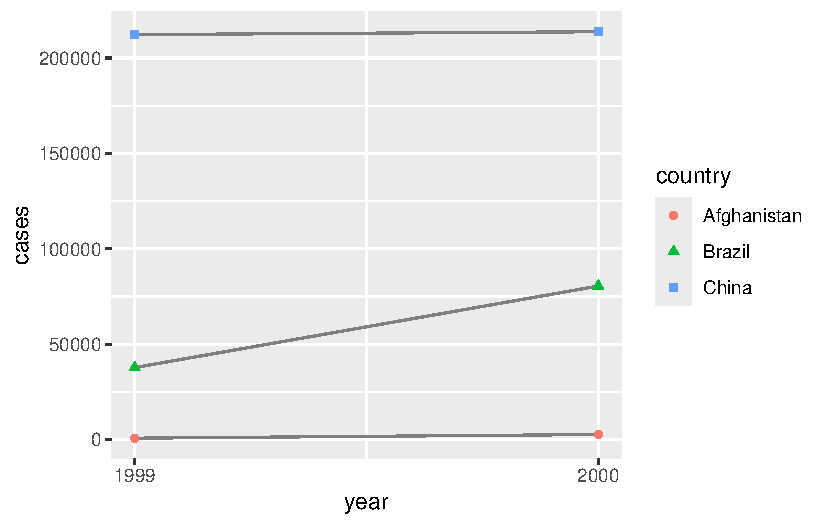
\includegraphics[keepaspectratio]{data-tidying_files/figure-pdf/unnamed-chunk-5-1.pdf}}

\subsection{Exercises}\label{exercises-8}

\textbf{1. For each of the sample tables, describe what each observation
and each column represents.}

\begin{Shaded}
\begin{Highlighting}[]
\NormalTok{table1}
\end{Highlighting}
\end{Shaded}

\begin{verbatim}
# A tibble: 6 x 4
  country      year  cases population
  <chr>       <dbl>  <dbl>      <dbl>
1 Afghanistan  1999    745   19987071
2 Afghanistan  2000   2666   20595360
3 Brazil       1999  37737  172006362
4 Brazil       2000  80488  174504898
5 China        1999 212258 1272915272
6 China        2000 213766 1280428583
\end{verbatim}

\begin{Shaded}
\begin{Highlighting}[]
\NormalTok{table2}
\end{Highlighting}
\end{Shaded}

\begin{verbatim}
# A tibble: 12 x 4
   country      year type            count
   <chr>       <dbl> <chr>           <dbl>
 1 Afghanistan  1999 cases             745
 2 Afghanistan  1999 population   19987071
 3 Afghanistan  2000 cases            2666
 4 Afghanistan  2000 population   20595360
 5 Brazil       1999 cases           37737
 6 Brazil       1999 population  172006362
 7 Brazil       2000 cases           80488
 8 Brazil       2000 population  174504898
 9 China        1999 cases          212258
10 China        1999 population 1272915272
11 China        2000 cases          213766
12 China        2000 population 1280428583
\end{verbatim}

\begin{Shaded}
\begin{Highlighting}[]
\NormalTok{table3}
\end{Highlighting}
\end{Shaded}

\begin{verbatim}
# A tibble: 6 x 3
  country      year rate             
  <chr>       <dbl> <chr>            
1 Afghanistan  1999 745/19987071     
2 Afghanistan  2000 2666/20595360    
3 Brazil       1999 37737/172006362  
4 Brazil       2000 80488/174504898  
5 China        1999 212258/1272915272
6 China        2000 213766/1280428583
\end{verbatim}

\begin{itemize}
\tightlist
\item
  \texttt{table1}: each row represents a country in a particular year.
  Cases and population are stored in separate columns.
\item
  \texttt{table2}: each row represents a country, year, and measurement
  type. Cases and population are stored in one \texttt{count} column,
  which makes this a longer format.
\item
  \texttt{table3}: each row represents a country in a particular year.
  Cases and population are combined into a character column called
  \texttt{rate}, which makes numerical calculations more difficult.
\end{itemize}

\textbf{2. Sketch out the process you'd use to calculate the rate for
\texttt{table2} and \texttt{table3}. You will need to perform four
operations:}

\begin{enumerate}
\def\labelenumi{\alph{enumi}.}
\tightlist
\item
  Extract the number of TB cases per country per year.
\item
  Extract the matching population per country per year.
\item
  Divide cases by population, and multiply by 10000.
\item
  Store back in the appropriate place.
\end{enumerate}

From ChatGPT:

\begin{quote}
For \texttt{table2}, I would group the data by country and year, extract
the count for cases and the count for population, divide cases by
population, multiply by 10,000, and store the result in a new
\texttt{rate} column. For \texttt{table3}, I would first separate the
\texttt{rate} column into cases and population, convert both values into
numbers, calculate cases divided by population times 10,000, and replace
the original text with the numerical rate.
\end{quote}

The code for \texttt{table2}:

\begin{Shaded}
\begin{Highlighting}[]
\NormalTok{table2 }\SpecialCharTok{|\textgreater{}}
  \FunctionTok{pivot\_wider}\NormalTok{(}
    \AttributeTok{names\_from =}\NormalTok{ type,}
    \AttributeTok{values\_from =}\NormalTok{ count}
\NormalTok{  ) }\SpecialCharTok{|\textgreater{}}
  \FunctionTok{mutate}\NormalTok{(}
    \AttributeTok{rate =}\NormalTok{ cases }\SpecialCharTok{/}\NormalTok{ population }\SpecialCharTok{*} \DecValTok{10000}
\NormalTok{  )}
\end{Highlighting}
\end{Shaded}

\begin{verbatim}
# A tibble: 6 x 5
  country      year  cases population  rate
  <chr>       <dbl>  <dbl>      <dbl> <dbl>
1 Afghanistan  1999    745   19987071 0.373
2 Afghanistan  2000   2666   20595360 1.29 
3 Brazil       1999  37737  172006362 2.19 
4 Brazil       2000  80488  174504898 4.61 
5 China        1999 212258 1272915272 1.67 
6 China        2000 213766 1280428583 1.67 
\end{verbatim}

\section{Lengthening data}\label{lengthening-data}

Pivoting transforms data into a tidy form: variables in columns and
observations in rows.

The tidyr functions for this are:

\begin{enumerate}
\def\labelenumi{\arabic{enumi}.}
\tightlist
\item
  \texttt{pivot\_longer()}
\item
  \texttt{pivot\_wider()}
\end{enumerate}

\subsection{Data in column names}\label{data-in-column-names}

\begin{Shaded}
\begin{Highlighting}[]
\NormalTok{billboard}
\end{Highlighting}
\end{Shaded}

\begin{verbatim}
# A tibble: 317 x 79
   artist     track date.entered   wk1   wk2   wk3   wk4   wk5   wk6   wk7   wk8
   <chr>      <chr> <date>       <dbl> <dbl> <dbl> <dbl> <dbl> <dbl> <dbl> <dbl>
 1 2 Pac      Baby~ 2000-02-26      87    82    72    77    87    94    99    NA
 2 2Ge+her    The ~ 2000-09-02      91    87    92    NA    NA    NA    NA    NA
 3 3 Doors D~ Kryp~ 2000-04-08      81    70    68    67    66    57    54    53
 4 3 Doors D~ Loser 2000-10-21      76    76    72    69    67    65    55    59
 5 504 Boyz   Wobb~ 2000-04-15      57    34    25    17    17    31    36    49
 6 98^0       Give~ 2000-08-19      51    39    34    26    26    19     2     2
 7 A*Teens    Danc~ 2000-07-08      97    97    96    95   100    NA    NA    NA
 8 Aaliyah    I Do~ 2000-01-29      84    62    51    41    38    35    35    38
 9 Aaliyah    Try ~ 2000-03-18      59    53    38    28    21    18    16    14
10 Adams, Yo~ Open~ 2000-08-26      76    76    74    69    68    67    61    58
# i 307 more rows
# i 68 more variables: wk9 <dbl>, wk10 <dbl>, wk11 <dbl>, wk12 <dbl>,
#   wk13 <dbl>, wk14 <dbl>, wk15 <dbl>, wk16 <dbl>, wk17 <dbl>, wk18 <dbl>,
#   wk19 <dbl>, wk20 <dbl>, wk21 <dbl>, wk22 <dbl>, wk23 <dbl>, wk24 <dbl>,
#   wk25 <dbl>, wk26 <dbl>, wk27 <dbl>, wk28 <dbl>, wk29 <dbl>, wk30 <dbl>,
#   wk31 <dbl>, wk32 <dbl>, wk33 <dbl>, wk34 <dbl>, wk35 <dbl>, wk36 <dbl>,
#   wk37 <dbl>, wk38 <dbl>, wk39 <dbl>, wk40 <dbl>, wk41 <dbl>, wk42 <dbl>, ...
\end{verbatim}

In the Billboard data, each row initially represents one song. The
weekly rankings are spread across the columns \texttt{wk1} to
\texttt{wk76}. The column names contain the week variable, while the
cell values contain the rank variable. \texttt{pivot\_longer()} converts
these weekly columns into rows, so that each row represents one song's
rank in one week.

\begin{Shaded}
\begin{Highlighting}[]
\NormalTok{billboard }\SpecialCharTok{|\textgreater{}}
  \FunctionTok{pivot\_longer}\NormalTok{(}
    \AttributeTok{cols =} \FunctionTok{starts\_with}\NormalTok{(}\StringTok{"wk"}\NormalTok{),}
    \AttributeTok{names\_to =} \StringTok{"week"}\NormalTok{,}
    \AttributeTok{values\_to =} \StringTok{"position"}
\NormalTok{  )}
\end{Highlighting}
\end{Shaded}

\begin{verbatim}
# A tibble: 24,092 x 5
   artist track                   date.entered week  position
   <chr>  <chr>                   <date>       <chr>    <dbl>
 1 2 Pac  Baby Don't Cry (Keep... 2000-02-26   wk1         87
 2 2 Pac  Baby Don't Cry (Keep... 2000-02-26   wk2         82
 3 2 Pac  Baby Don't Cry (Keep... 2000-02-26   wk3         72
 4 2 Pac  Baby Don't Cry (Keep... 2000-02-26   wk4         77
 5 2 Pac  Baby Don't Cry (Keep... 2000-02-26   wk5         87
 6 2 Pac  Baby Don't Cry (Keep... 2000-02-26   wk6         94
 7 2 Pac  Baby Don't Cry (Keep... 2000-02-26   wk7         99
 8 2 Pac  Baby Don't Cry (Keep... 2000-02-26   wk8         NA
 9 2 Pac  Baby Don't Cry (Keep... 2000-02-26   wk9         NA
10 2 Pac  Baby Don't Cry (Keep... 2000-02-26   wk10        NA
# i 24,082 more rows
\end{verbatim}

Or a different way of selecting the columns:

\begin{Shaded}
\begin{Highlighting}[]
\NormalTok{billboard }\SpecialCharTok{|\textgreater{}}
  \FunctionTok{pivot\_longer}\NormalTok{(}
    \AttributeTok{cols =} \SpecialCharTok{!}\FunctionTok{c}\NormalTok{(artist, track, date.entered),}
    \AttributeTok{names\_to =} \StringTok{"week"}\NormalTok{,}
    \AttributeTok{values\_to =} \StringTok{"rank"}
\NormalTok{  )}
\end{Highlighting}
\end{Shaded}

\begin{verbatim}
# A tibble: 24,092 x 5
   artist track                   date.entered week   rank
   <chr>  <chr>                   <date>       <chr> <dbl>
 1 2 Pac  Baby Don't Cry (Keep... 2000-02-26   wk1      87
 2 2 Pac  Baby Don't Cry (Keep... 2000-02-26   wk2      82
 3 2 Pac  Baby Don't Cry (Keep... 2000-02-26   wk3      72
 4 2 Pac  Baby Don't Cry (Keep... 2000-02-26   wk4      77
 5 2 Pac  Baby Don't Cry (Keep... 2000-02-26   wk5      87
 6 2 Pac  Baby Don't Cry (Keep... 2000-02-26   wk6      94
 7 2 Pac  Baby Don't Cry (Keep... 2000-02-26   wk7      99
 8 2 Pac  Baby Don't Cry (Keep... 2000-02-26   wk8      NA
 9 2 Pac  Baby Don't Cry (Keep... 2000-02-26   wk9      NA
10 2 Pac  Baby Don't Cry (Keep... 2000-02-26   wk10     NA
# i 24,082 more rows
\end{verbatim}

\texttt{pivot\_longer()} converts the columns beginning with \texttt{wk}
into rows. The old column names are stored in a new \texttt{week}
column, while the ranking values are stored in a new \texttt{rank}
column.

\begin{itemize}
\tightlist
\item
  \texttt{cols} identifies the columns to pivot.
\item
  \texttt{names\_to} gives a name to the new column containing the old
  column names.
\item
  \texttt{values\_to} gives a name to the new column containing the old
  cell values.
\end{itemize}

\textbf{Structural missing values} occur because of how the data is
organized, rather than because an expected value is unknown. In the
Billboard data, \texttt{NA} means a song was not in the Top 100 during
that week. \texttt{values\_drop\_na\ =\ TRUE} removes these unnecessary
\texttt{NA} rows when using \texttt{pivot\_longer()}.

\begin{Shaded}
\begin{Highlighting}[]
\NormalTok{billboard }\SpecialCharTok{|\textgreater{}}
  \FunctionTok{pivot\_longer}\NormalTok{(}
    \AttributeTok{cols =} \FunctionTok{starts\_with}\NormalTok{(}\StringTok{"wk"}\NormalTok{),}
    \AttributeTok{values\_to =} \StringTok{"position"}\NormalTok{,}
    \AttributeTok{names\_to =} \StringTok{"week"}\NormalTok{,}
    \AttributeTok{values\_drop\_na =} \ConstantTok{TRUE}
\NormalTok{  )}
\end{Highlighting}
\end{Shaded}

\begin{verbatim}
# A tibble: 5,307 x 5
   artist  track                   date.entered week  position
   <chr>   <chr>                   <date>       <chr>    <dbl>
 1 2 Pac   Baby Don't Cry (Keep... 2000-02-26   wk1         87
 2 2 Pac   Baby Don't Cry (Keep... 2000-02-26   wk2         82
 3 2 Pac   Baby Don't Cry (Keep... 2000-02-26   wk3         72
 4 2 Pac   Baby Don't Cry (Keep... 2000-02-26   wk4         77
 5 2 Pac   Baby Don't Cry (Keep... 2000-02-26   wk5         87
 6 2 Pac   Baby Don't Cry (Keep... 2000-02-26   wk6         94
 7 2 Pac   Baby Don't Cry (Keep... 2000-02-26   wk7         99
 8 2Ge+her The Hardest Part Of ... 2000-09-02   wk1         91
 9 2Ge+her The Hardest Part Of ... 2000-09-02   wk2         87
10 2Ge+her The Hardest Part Of ... 2000-09-02   wk3         92
# i 5,297 more rows
\end{verbatim}

To make computation easier, we can convert the values of \texttt{week}
from character strings to numbers, using \texttt{mutate()} and
\texttt{readr::parse\_number()}:

\begin{Shaded}
\begin{Highlighting}[]
\NormalTok{billboard\_longer }\OtherTok{\textless{}{-}}\NormalTok{ billboard }\SpecialCharTok{|\textgreater{}}
  \FunctionTok{pivot\_longer}\NormalTok{(}
    \AttributeTok{cols =} \FunctionTok{starts\_with}\NormalTok{(}\StringTok{"wk"}\NormalTok{),}
    \AttributeTok{names\_to =} \StringTok{"week"}\NormalTok{,}
    \AttributeTok{values\_to =} \StringTok{"position"}\NormalTok{,}
    \AttributeTok{values\_drop\_na =} \ConstantTok{TRUE}
\NormalTok{  ) }\SpecialCharTok{|\textgreater{}}
  \FunctionTok{mutate}\NormalTok{(}\AttributeTok{week =} \FunctionTok{parse\_number}\NormalTok{(week))}

\NormalTok{billboard\_longer}
\end{Highlighting}
\end{Shaded}

\begin{verbatim}
# A tibble: 5,307 x 5
   artist  track                   date.entered  week position
   <chr>   <chr>                   <date>       <dbl>    <dbl>
 1 2 Pac   Baby Don't Cry (Keep... 2000-02-26       1       87
 2 2 Pac   Baby Don't Cry (Keep... 2000-02-26       2       82
 3 2 Pac   Baby Don't Cry (Keep... 2000-02-26       3       72
 4 2 Pac   Baby Don't Cry (Keep... 2000-02-26       4       77
 5 2 Pac   Baby Don't Cry (Keep... 2000-02-26       5       87
 6 2 Pac   Baby Don't Cry (Keep... 2000-02-26       6       94
 7 2 Pac   Baby Don't Cry (Keep... 2000-02-26       7       99
 8 2Ge+her The Hardest Part Of ... 2000-09-02       1       91
 9 2Ge+her The Hardest Part Of ... 2000-09-02       2       87
10 2Ge+her The Hardest Part Of ... 2000-09-02       3       92
# i 5,297 more rows
\end{verbatim}

\texttt{pivot\_longer()} initially creates \texttt{week} as character
values such as ``wk1'' and ``wk2''. \texttt{mutate()} with
\texttt{parse\_number()} extracts the numbers and converts \texttt{week}
to a numeric variable, making future calculations easier.

We can now visualize how song ranks vary over time:

\begin{Shaded}
\begin{Highlighting}[]
\NormalTok{billboard\_longer }\SpecialCharTok{|\textgreater{}}
  \FunctionTok{ggplot}\NormalTok{(}\FunctionTok{aes}\NormalTok{(week, position, }\AttributeTok{group =}\NormalTok{ track)) }\SpecialCharTok{+}
  \FunctionTok{geom\_line}\NormalTok{(}\AttributeTok{alpha =} \FloatTok{0.25}\NormalTok{) }\SpecialCharTok{+}
  \FunctionTok{scale\_y\_reverse}\NormalTok{()}
\end{Highlighting}
\end{Shaded}

\pandocbounded{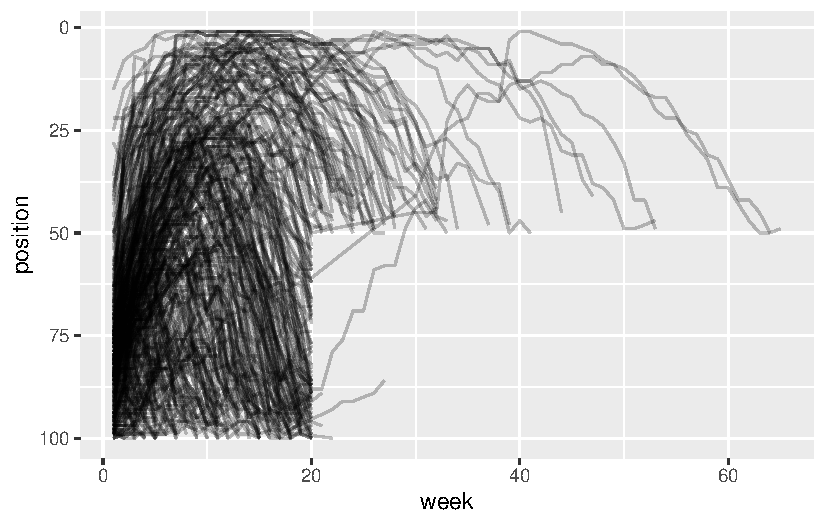
\includegraphics[keepaspectratio]{data-tidying_files/figure-pdf/unnamed-chunk-13-1.pdf}}

\subsection{How does pivoting work?}\label{how-does-pivoting-work}

Suppose we have 3 patients, each with 2 blood pressure readings:

\begin{Shaded}
\begin{Highlighting}[]
\NormalTok{df }\OtherTok{\textless{}{-}} \FunctionTok{tribble}\NormalTok{(}
  \SpecialCharTok{\textasciitilde{}}\NormalTok{id,  }\SpecialCharTok{\textasciitilde{}}\NormalTok{bp1, }\SpecialCharTok{\textasciitilde{}}\NormalTok{bp2,}
  \StringTok{"A"}\NormalTok{,  }\DecValTok{100}\NormalTok{,  }\DecValTok{120}\NormalTok{,}
  \StringTok{"B"}\NormalTok{,  }\DecValTok{140}\NormalTok{,  }\DecValTok{115}\NormalTok{,}
  \StringTok{"C"}\NormalTok{,  }\DecValTok{120}\NormalTok{,  }\DecValTok{125}
\NormalTok{)}
\end{Highlighting}
\end{Shaded}

We want our new dataset to have three variables: \texttt{id} (which
already exists), \texttt{measurement} (the column names), and
\texttt{value} (the cell values). To achieve this, we pivot \texttt{df}
longer:

\begin{Shaded}
\begin{Highlighting}[]
\NormalTok{df }\SpecialCharTok{|\textgreater{}}
  \FunctionTok{pivot\_longer}\NormalTok{(}
    \AttributeTok{cols =}\NormalTok{ bp1}\SpecialCharTok{:}\NormalTok{bp2,}
    \AttributeTok{names\_to =} \StringTok{"measurement"}\NormalTok{,}
    \AttributeTok{values\_to =} \StringTok{"value"}
\NormalTok{  )}
\end{Highlighting}
\end{Shaded}

\begin{verbatim}
# A tibble: 6 x 3
  id    measurement value
  <chr> <chr>       <dbl>
1 A     bp1           100
2 A     bp2           120
3 B     bp1           140
4 B     bp2           115
5 C     bp1           120
6 C     bp2           125
\end{verbatim}

\bookmarksetup{startatroot}

\chapter{Summary}\label{summary}

In summary, this book has no content whatsoever.

\begin{Shaded}
\begin{Highlighting}[]
\DecValTok{1} \SpecialCharTok{+} \DecValTok{1}
\end{Highlighting}
\end{Shaded}

\begin{verbatim}
[1] 2
\end{verbatim}

\bookmarksetup{startatroot}

\chapter*{References}\label{references}
\addcontentsline{toc}{chapter}{References}

\markboth{References}{References}

\protect\phantomsection\label{refs}




\end{document}
